\documentclass[a4paper,UKenglish,cleveref, autoref]{lipics-v2019}

\usepackage[utf8]{inputenc}
\usepackage[T1]{fontenc}
\usepackage{amsmath,amsfonts,amssymb,amsthm}
\usepackage{parskip}
\usepackage{enumerate}
\usepackage{xspace}
%\usepackage{framed}
\usepackage{multicol}
\usepackage[dvipsnames]{xcolor}
\usepackage[noend]{algpseudocode}
\usepackage{algorithm}
\usepackage[normalem]{ulem}

\usepackage{tikz}
\usetikzlibrary{quotes}
\usetikzlibrary{calc}

\tikzset{wire/.style={draw, inner sep=0, minimum size=0.5cm}}
\tikzset{extra box/.style={draw, minimum size=0.6cm}}
\tikzset{every edge/.style={shorten >=0.5mm, draw}}

\hypersetup{colorlinks=true,linkcolor=blue,urlcolor=blue}

\newcommand{\bits}{\left\{0, 1\right\}}
\newcommand{\bigO}[1]{\ensuremath{\mathcal{O}\left( #1 \right)} }
\newcommand{\bigOsoft}[1]{\ensuremath{\mathcal{\tilde O}\left( #1 \right)} }
\newcommand{\bigOmega}[1]{\ensuremath{\Omega\left( #1 \right)} }
\newcommand{\bigTheta}[1]{\ensuremath{\Theta\left( #1 \right)} }
\newcommand{\Prob}{\mathrm{Pr}}

\newcommand{\red}{\color{red}}
\newcommand{\FIXME}{{\red \textbf{FIXME}}\xspace}
\newcommand{\TODO}[1]{{\red \textbf{TODO}:} #1\xspace}

\bibliographystyle{plainurl}% the mandatory bibstyle

\title{\textsc{MIDTERM} Is a Deterministic Technique to Exit Recursive Mazes}

\author{Charles Bouillaguet}{LIP6 laboratory, Sorbonne Université, Paris, France}{charles.bouillaguet@lip6.fr}{https://orcid.org/0000-0001-9416-6244}{} 
\author{Orel Cosseron}{Independent researcher}{orel.cosseron@ens-lyon.fr}{https://orcid.org/0000-0001-9481-8935}{}

\authorrunning{C. Bouillaguet and O. Cosseron}

\Copyright{Charles Bouillaguet and Orel Cosseron}

\ccsdesc[500]{Theory of computation~Grammars and context-free languages}
\ccsdesc[500]{Theory of computation~Graph algorithms analysis}

% \ccsdesc[100]{Theory of computation~Computational complexity and cryptography}
% \ccsdesc[100]{Theory of computation~Design and analysis of algorithms}% Please choose ACM 2012 classifications from https://dl.acm.org/ccs/ccs_flat.cfm 

\keywords{Quantum computing, blockchains, IA, pushdown automaton, reachability, graph rewriting, addition chains, recursive maze, $(\lambda x. xx)(\lambda x. xx)$}

%\supplement{Source code available at : \url{https://gitlab.lip6.fr/almasty/mq/}}

% \funding{We acknowledge nfinancial support from the French Agence Nationale de la
%   Recherche under projects ``PostCryptum'' (ANR20-ASTR-0011) and ``GORILLA''
%   (ANR-20-CE39-0002).}

\hideLIPIcs
\nolinenumbers

\begin{document}
\maketitle

\begin{abstract}
  A recursive maze is a maze that contains copies of itself
  (that themselves contain copies of themselves, etc.). To exit
  the maze or reach the goal, each recursive block that has been entered must
  be exited. These once-popular puzzles are difficult to solve by hand, and this
  begs for an algorithmic solution.

  It has been observed many times in the past that a recursive maze can be
  represented by a deterministic pushdown automaton. Finding a path, possibly
  the shortest, that leads to an exit therefore reduces to finding a word in a
  context-free language described by such an automaton. The problem is
  well-known to be decidable, and there is a classical algorithm for this
  task. We present a new algorithm, \textsc{Midterm}, with improved complexity
  compared to existing solutions.

  \textsc{Midterm} improves on a previous attempt called \textsc{Longterm}
  (Obviously Not a Good Technique to Exit Recursive Mazes).
\end{abstract}


\section{Introduction}

A \emph{recursive maze} is a maze that contains copies of itself. As the adage
goes, a picture is worth a thousand words, and the concept is therefore best
illustrated by Figures~\ref{fig:jpwolf} and~\ref{fig:later}. Recursive mazes
have been invented by Mark J. P. Wolf (univ. Wisconsin) and the first one was
published in 1996 under the name ``\emph{fractal maze}'' (\emph{Extropy} \#17,
p. 67, available in the
\href{https://archive.org/details/extropy-17/page/66/mode/2up}{internet
  archive}). Similar puzzles later appeared both in print and online. Recursive
mazes are notoriously difficult to solve by hand, without taking notes and/or
using an \textit{ad hoc} computer program to track one's position in the
maze. Several such program exist, notably to play in a web browser, such as
\begin{center}
  \url{https://amurielagi.github.io/fractal-maze/}
\end{center}
or
\begin{center}
  \verb|\begin{shameless-advertisement}| \hspace{5cm}~\\
    \hspace{2cm}\url{https://orelcosseron.github.io/fractal-maze/}\\
  \verb|\end{shameless-advertisement}| \hspace{5cm}~
\end{center}

\begin{figure}
  \includegraphics[width=0.59\textwidth]{FractalMaze95.png}
  \includegraphics[width=0.39\textwidth]{fractal1.png}
  \caption{Two early recursive mazes designed by Mark J. P. Wolf. First published in \href{https://archive.org/details/extropy-17/page/66/mode/2up}{Extropy \#17, Fall 1996, page 67} (left) and in the "Bogglers" column of the June 2004 issue of Discover Magazine, page 86 (right). See also the book~\cite{WolfBook} by the same author. \label{fig:jpwolf}}
\end{figure}

\begin{figure}
  \includegraphics[width=0.48\textwidth]{Alice.png}
  \includegraphics[width=0.48\textwidth]{circular.pdf}
  \caption{Two other recursive mazes designed by Mike Earnest (published on July 2016 as a \href{https://puzzling.stackexchange.com/questions/37675/alice-and-the-fractal-hedge-maze}{StackExchange puzzle}, left) and Tristan ``Siggy'' Miller (published on October 2010 on the \href{https://skepticsplay.blogspot.com/2010/10/fractal-maze.html}{Skeptic's Play blog}, right). \label{fig:later}}
\end{figure}

At first glance, a recursive maze looks like the floor plan of an integrated
circuit, that itself contains ``boxes'' representing inner integrated
circuits. There are \emph{wires} connecting the ``outer'' IO pins (on the edge
of the circuit) to the ``inner'' IO pins of the boxes contained inside. The
boxes are often distinguished with capital letters. There are also special
locations, such as $\oplus$ and $\ominus$ in Fig.~\ref{fig:jpwolf}, or the
starting point (``you are here'') in Fig.~\ref{fig:later}. The aim of the puzzle
consists in following the wires from point $A$ to point $B$: from $\ominus$ to
$\oplus$ in Fig.~\ref{fig:jpwolf}, from the starting point to the outside or to
the finish line in Fig.~\ref{fig:later}. The trick is that, when following a
wire, we may hit one of the inner boxes. In this case, we ``enter'' the box,
which is a copy of the whole maze. Each entered box must be exited, by reaching
one of its outer IO pin.

This is where the real fun begins. For one, exiting may not be possible at
all. Consider for instance the innocent-looking maze:
\begin{center}
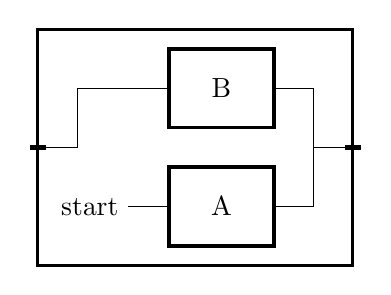
\begin{tikzpicture}
  % special
  \node at (0.66, 0.75) (start) {start};
  \draw (start) -- (5/3, 0.75);

  \draw[very thick] (0, 0) rectangle +(4, 3);
  \draw[ultra thick] (0, 1.5) +(-0.1, 0) -- +(0.1, 0);
  \draw[ultra thick] (4, 1.5) +(-0.1, 0) -- +(0.1, 0);

  % inside paths
  \draw (0, 1.5) -- (0.5, 1.5) -- (0.5, 2.25) -- (5/3, 2.25);
  \draw (3, 2.25) -| (3.5, 1.5);
  \draw (3, 0.75) -| (3.5, 1.5);
  \draw (3.5, 1.5) -- (4, 1.5);

  \begin{scope}[xshift=1.6667cm, yshift=0.25cm, scale=0.33333]
  \draw[very thick] (0, 0) rectangle node {A} +(4, 3);
  \end{scope}  

  \begin{scope}[xshift=1.6667cm, yshift=1.75cm, scale=0.33333]
  \draw[very thick] (0, 0) rectangle node {B} +(4, 3);
  \end{scope}  
\end{tikzpicture}
\end{center}

From the starting point, one has to enter A (from the left). But from there, the
only option is to follow the wire that leads to B, and enter on the left. From
there, we are stuck in an infinite loop of entering B, and there is no way that
we can exit the maze. In fact, the maze expands to:

\begin{center}
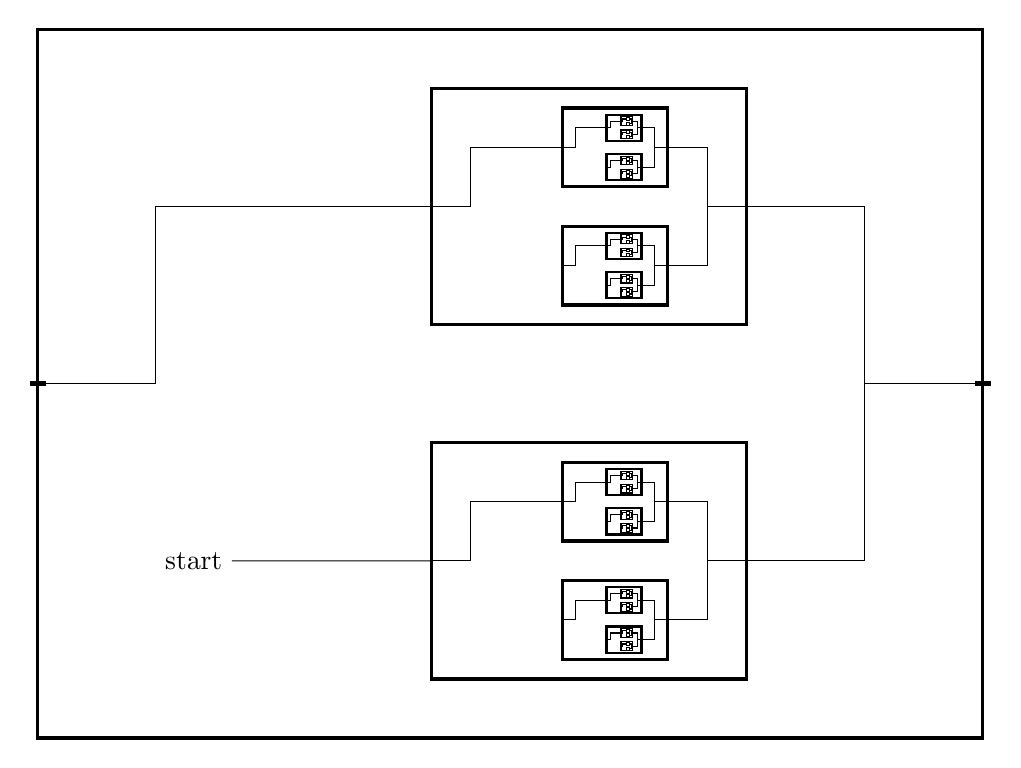
\begin{tikzpicture}[scale=3]
  % special
  \node at (0.66, 0.75) (start) {start};
  \draw (start) -- (5/3, 0.75);

  \draw[very thick] (0, 0) rectangle +(4, 3);
  \draw[ultra thick] (0, 1.5) +(-0.0333, 0) -- +(0.0333, 0);
  \draw[ultra thick] (4, 1.5) +(-0.0333, 0) -- +(0.0333, 0);
  \draw (0, 1.5) -- (0.5, 1.5) -- (0.5, 2.25) -- (5/3, 2.25);
  \draw (3, 2.25) -| (3.5, 1.5);
  \draw (3, 0.75) -| (3.5, 1.5);
  \draw (3.5, 1.5) -- (4, 1.5);

  % depth 1
  \begin{scope}[xshift=1.6667cm, yshift=0.25cm, scale=0.33333]
  \draw[very thick] (0, 0) rectangle +(4, 3);
  \draw (0, 1.5) -- (0.5, 1.5) -- (0.5, 2.25) -- (5/3, 2.25);
  \draw (3, 2.25) -| (3.5, 1.5);
  \draw (3, 0.75) -| (3.5, 1.5);
  \draw (3.5, 1.5) -- (4, 1.5);

  % depth 2
  \begin{scope}[xshift=1.6667cm, yshift=0.25cm, scale=0.33333]
  \draw[very thick] (0, 0) rectangle +(4, 3);
  \draw (0, 1.5) -- (0.5, 1.5) -- (0.5, 2.25) -- (5/3, 2.25);
  \draw (3, 2.25) -| (3.5, 1.5);
  \draw (3, 0.75) -| (3.5, 1.5);
  \draw (3.5, 1.5) -- (4, 1.5);

  % depth 3
  \begin{scope}[xshift=1.6667cm, yshift=0.25cm, scale=0.33333]
  \draw[thick] (0, 0) rectangle +(4, 3);
  \draw (0, 1.5) -- (0.5, 1.5) -- (0.5, 2.25) -- (5/3, 2.25);
  \draw (3, 2.25) -| (3.5, 1.5);
  \draw (3, 0.75) -| (3.5, 1.5);
  \draw (3.5, 1.5) -- (4, 1.5);

  % depth 4
  \begin{scope}[xshift=1.6667cm, yshift=0.25cm, scale=0.33333]
  \draw[] (0, 0) rectangle +(4, 3);
  \draw (0, 1.5) -- (0.5, 1.5) -- (0.5, 2.25) -- (5/3, 2.25);
  \draw (3, 2.25) -| (3.5, 1.5);
  \draw (3, 0.75) -| (3.5, 1.5);
  \draw (3.5, 1.5) -- (4, 1.5);

  % end of recursion
  \begin{scope}[xshift=1.6667cm, yshift=0.25cm, scale=0.33333]
    \draw[very thin] (0, 0) rectangle +(4, 3);
  \end{scope}
  \begin{scope}[xshift=1.6667cm, yshift=1.75cm, scale=0.33333]
    \draw[very thin] (0, 0) rectangle +(4, 3);
  \end{scope}
\end{scope}

  % depth 4
  \begin{scope}[xshift=1.6667cm, yshift=1.75cm, scale=0.33333]
  \draw[] (0, 0) rectangle +(4, 3);
  \draw (0, 1.5) -- (0.5, 1.5) -- (0.5, 2.25) -- (5/3, 2.25);
  \draw (3, 2.25) -| (3.5, 1.5);
  \draw (3, 0.75) -| (3.5, 1.5);
  \draw (3.5, 1.5) -- (4, 1.5);
  % end of recursion
  \begin{scope}[xshift=1.6667cm, yshift=0.25cm, scale=0.33333]
    \draw[very thin] (0, 0) rectangle +(4, 3);
  \end{scope}
  \begin{scope}[xshift=1.6667cm, yshift=1.75cm, scale=0.33333]
    \draw[very thin] (0, 0) rectangle +(4, 3);
  \end{scope}
  \end{scope}
  \end{scope}

  % depth 3
  \begin{scope}[xshift=1.6667cm, yshift=1.75cm, scale=0.33333]
  \draw[thick] (0, 0) rectangle +(4, 3);
  \draw (0, 1.5) -- (0.5, 1.5) -- (0.5, 2.25) -- (5/3, 2.25);
  \draw (3, 2.25) -| (3.5, 1.5);
  \draw (3, 0.75) -| (3.5, 1.5);
  \draw (3.5, 1.5) -- (4, 1.5);

  % depth 4
  \begin{scope}[xshift=1.6667cm, yshift=0.25cm, scale=0.33333]
  \draw[] (0, 0) rectangle +(4, 3);
  \draw (0, 1.5) -- (0.5, 1.5) -- (0.5, 2.25) -- (5/3, 2.25);
  \draw (3, 2.25) -| (3.5, 1.5);
  \draw (3, 0.75) -| (3.5, 1.5);
  \draw (3.5, 1.5) -- (4, 1.5);
  % end of recursion
  \begin{scope}[xshift=1.6667cm, yshift=0.25cm, scale=0.33333]
    \draw[very thin] (0, 0) rectangle +(4, 3);
  \end{scope}
  \begin{scope}[xshift=1.6667cm, yshift=1.75cm, scale=0.33333]
    \draw[very thin] (0, 0) rectangle +(4, 3);
  \end{scope}
  \end{scope}

  % depth 4
  \begin{scope}[xshift=1.6667cm, yshift=1.75cm, scale=0.33333]
  \draw[] (0, 0) rectangle +(4, 3);
  \draw (0, 1.5) -- (0.5, 1.5) -- (0.5, 2.25) -- (5/3, 2.25);
  \draw (3, 2.25) -| (3.5, 1.5);
  \draw (3, 0.75) -| (3.5, 1.5);
  \draw (3.5, 1.5) -- (4, 1.5);
  % end of recursion
  \begin{scope}[xshift=1.6667cm, yshift=0.25cm, scale=0.33333]
    \draw[very thin] (0, 0) rectangle +(4, 3);
  \end{scope}
  \begin{scope}[xshift=1.6667cm, yshift=1.75cm, scale=0.33333]
    \draw[very thin] (0, 0) rectangle +(4, 3);
  \end{scope}
  \end{scope}
  \end{scope}  
  \end{scope}

  % depth 2
  \begin{scope}[xshift=1.6667cm, yshift=1.75cm, scale=0.33333]
  \draw[very thick] (0, 0) rectangle +(4, 3);
  \draw (0, 1.5) -- (0.5, 1.5) -- (0.5, 2.25) -- (5/3, 2.25);
  \draw (3, 2.25) -| (3.5, 1.5);
  \draw (3, 0.75) -| (3.5, 1.5);
  \draw (3.5, 1.5) -- (4, 1.5);

  % depth 3
  \begin{scope}[xshift=1.6667cm, yshift=0.25cm, scale=0.33333]
  \draw[thick] (0, 0) rectangle +(4, 3);
  \draw (0, 1.5) -- (0.5, 1.5) -- (0.5, 2.25) -- (5/3, 2.25);
  \draw (3, 2.25) -| (3.5, 1.5);
  \draw (3, 0.75) -| (3.5, 1.5);
  \draw (3.5, 1.5) -- (4, 1.5);

  % depth 4
  \begin{scope}[xshift=1.6667cm, yshift=0.25cm, scale=0.33333]
  \draw[] (0, 0) rectangle +(4, 3);
  \draw (0, 1.5) -- (0.5, 1.5) -- (0.5, 2.25) -- (5/3, 2.25);
  \draw (3, 2.25) -| (3.5, 1.5);
  \draw (3, 0.75) -| (3.5, 1.5);
  \draw (3.5, 1.5) -- (4, 1.5);
  % end of recursion
  \begin{scope}[xshift=1.6667cm, yshift=0.25cm, scale=0.33333]
    \draw[very thin] (0, 0) rectangle +(4, 3);
  \end{scope}
  \begin{scope}[xshift=1.6667cm, yshift=1.75cm, scale=0.33333]
    \draw[very thin] (0, 0) rectangle +(4, 3);
  \end{scope}
  \end{scope}

  % depth 4
  \begin{scope}[xshift=1.6667cm, yshift=1.75cm, scale=0.33333]
  \draw[] (0, 0) rectangle +(4, 3);
  \draw (0, 1.5) -- (0.5, 1.5) -- (0.5, 2.25) -- (5/3, 2.25);
  \draw (3, 2.25) -| (3.5, 1.5);
  \draw (3, 0.75) -| (3.5, 1.5);
  \draw (3.5, 1.5) -- (4, 1.5);
  % end of recursion
  \begin{scope}[xshift=1.6667cm, yshift=0.25cm, scale=0.33333]
    \draw[very thin] (0, 0) rectangle +(4, 3);
  \end{scope}
  \begin{scope}[xshift=1.6667cm, yshift=1.75cm, scale=0.33333]
    \draw[very thin] (0, 0) rectangle +(4, 3);
  \end{scope}
  \end{scope}
  \end{scope}

  % depth 3
  \begin{scope}[xshift=1.6667cm, yshift=1.75cm, scale=0.33333]
  \draw[thick] (0, 0) rectangle +(4, 3);
  \draw (0, 1.5) -- (0.5, 1.5) -- (0.5, 2.25) -- (5/3, 2.25);
  \draw (3, 2.25) -| (3.5, 1.5);
  \draw (3, 0.75) -| (3.5, 1.5);
  \draw (3.5, 1.5) -- (4, 1.5);

  % depth 4
  \begin{scope}[xshift=1.6667cm, yshift=0.25cm, scale=0.33333]
  \draw[] (0, 0) rectangle +(4, 3);
  \draw (0, 1.5) -- (0.5, 1.5) -- (0.5, 2.25) -- (5/3, 2.25);
  \draw (3, 2.25) -| (3.5, 1.5);
  \draw (3, 0.75) -| (3.5, 1.5);
  \draw (3.5, 1.5) -- (4, 1.5);
  % end of recursion
  \begin{scope}[xshift=1.6667cm, yshift=0.25cm, scale=0.33333]
    \draw[very thin] (0, 0) rectangle +(4, 3);
  \end{scope}
  \begin{scope}[xshift=1.6667cm, yshift=1.75cm, scale=0.33333]
    \draw[very thin] (0, 0) rectangle +(4, 3);
  \end{scope}
  \end{scope}

  % depth 4
  \begin{scope}[xshift=1.6667cm, yshift=1.75cm, scale=0.33333]
  \draw[] (0, 0) rectangle +(4, 3);
  \draw (0, 1.5) -- (0.5, 1.5) -- (0.5, 2.25) -- (5/3, 2.25);
  \draw (3, 2.25) -| (3.5, 1.5);
  \draw (3, 0.75) -| (3.5, 1.5);
  \draw (3.5, 1.5) -- (4, 1.5);
  % end of recursion
  \begin{scope}[xshift=1.6667cm, yshift=0.25cm, scale=0.33333]
    \draw[very thin] (0, 0) rectangle +(4, 3);
  \end{scope}
  \begin{scope}[xshift=1.6667cm, yshift=1.75cm, scale=0.33333]
    \draw[very thin] (0, 0) rectangle +(4, 3);
  \end{scope}
  \end{scope}
  \end{scope}  
  \end{scope}
  \end{scope}

  % depth 1
  \begin{scope}[xshift=1.6667cm, yshift=1.75cm, scale=0.33333]
  \draw[very thick] (0, 0) rectangle +(4, 3);
  \draw (0, 1.5) -- (0.5, 1.5) -- (0.5, 2.25) -- (5/3, 2.25);
  \draw (3, 2.25) -| (3.5, 1.5);
  \draw (3, 0.75) -| (3.5, 1.5);
  \draw (3.5, 1.5) -- (4, 1.5);

  % depth 2
  \begin{scope}[xshift=1.6667cm, yshift=0.25cm, scale=0.33333]
  \draw[very thick] (0, 0) rectangle +(4, 3);
  \draw (0, 1.5) -- (0.5, 1.5) -- (0.5, 2.25) -- (5/3, 2.25);
  \draw (3, 2.25) -| (3.5, 1.5);
  \draw (3, 0.75) -| (3.5, 1.5);
  \draw (3.5, 1.5) -- (4, 1.5);

  % depth 3
  \begin{scope}[xshift=1.6667cm, yshift=0.25cm, scale=0.33333]
  \draw[thick] (0, 0) rectangle +(4, 3);
  \draw (0, 1.5) -- (0.5, 1.5) -- (0.5, 2.25) -- (5/3, 2.25);
  \draw (3, 2.25) -| (3.5, 1.5);
  \draw (3, 0.75) -| (3.5, 1.5);
  \draw (3.5, 1.5) -- (4, 1.5);

  % depth 4
  \begin{scope}[xshift=1.6667cm, yshift=0.25cm, scale=0.33333]
  \draw[] (0, 0) rectangle +(4, 3);
  \draw (0, 1.5) -- (0.5, 1.5) -- (0.5, 2.25) -- (5/3, 2.25);
  \draw (3, 2.25) -| (3.5, 1.5);
  \draw (3, 0.75) -| (3.5, 1.5);
  \draw (3.5, 1.5) -- (4, 1.5);
  % end of recursion
  \begin{scope}[xshift=1.6667cm, yshift=0.25cm, scale=0.33333]
    \draw[very thin] (0, 0) rectangle +(4, 3);
  \end{scope}
  \begin{scope}[xshift=1.6667cm, yshift=1.75cm, scale=0.33333]
    \draw[very thin] (0, 0) rectangle +(4, 3);
  \end{scope}
  \end{scope}

  % depth 4
  \begin{scope}[xshift=1.6667cm, yshift=1.75cm, scale=0.33333]
  \draw[] (0, 0) rectangle +(4, 3);
  \draw (0, 1.5) -- (0.5, 1.5) -- (0.5, 2.25) -- (5/3, 2.25);
  \draw (3, 2.25) -| (3.5, 1.5);
  \draw (3, 0.75) -| (3.5, 1.5);
  \draw (3.5, 1.5) -- (4, 1.5);
  % end of recursion
  \begin{scope}[xshift=1.6667cm, yshift=0.25cm, scale=0.33333]
    \draw[very thin] (0, 0) rectangle +(4, 3);
  \end{scope}
  \begin{scope}[xshift=1.6667cm, yshift=1.75cm, scale=0.33333]
    \draw[very thin] (0, 0) rectangle +(4, 3);
  \end{scope}
  \end{scope}
  \end{scope}

  % depth 3
  \begin{scope}[xshift=1.6667cm, yshift=1.75cm, scale=0.33333]
  \draw[thick] (0, 0) rectangle +(4, 3);
  \draw (0, 1.5) -- (0.5, 1.5) -- (0.5, 2.25) -- (5/3, 2.25);
  \draw (3, 2.25) -| (3.5, 1.5);
  \draw (3, 0.75) -| (3.5, 1.5);
  \draw (3.5, 1.5) -- (4, 1.5);

  % depth 4
  \begin{scope}[xshift=1.6667cm, yshift=0.25cm, scale=0.33333]
  \draw[] (0, 0) rectangle +(4, 3);
  \draw (0, 1.5) -- (0.5, 1.5) -- (0.5, 2.25) -- (5/3, 2.25);
  \draw (3, 2.25) -| (3.5, 1.5);
  \draw (3, 0.75) -| (3.5, 1.5);
  \draw (3.5, 1.5) -- (4, 1.5);
  % end of recursion
  \begin{scope}[xshift=1.6667cm, yshift=0.25cm, scale=0.33333]
    \draw[very thin] (0, 0) rectangle +(4, 3);
  \end{scope}
  \begin{scope}[xshift=1.6667cm, yshift=1.75cm, scale=0.33333]
    \draw[very thin] (0, 0) rectangle +(4, 3);
  \end{scope}
  \end{scope}

  % depth 4
  \begin{scope}[xshift=1.6667cm, yshift=1.75cm, scale=0.33333]
  \draw[] (0, 0) rectangle +(4, 3);
  \draw (0, 1.5) -- (0.5, 1.5) -- (0.5, 2.25) -- (5/3, 2.25);
  \draw (3, 2.25) -| (3.5, 1.5);
  \draw (3, 0.75) -| (3.5, 1.5);
  \draw (3.5, 1.5) -- (4, 1.5);
  % end of recursion
  \begin{scope}[xshift=1.6667cm, yshift=0.25cm, scale=0.33333]
    \draw[very thin] (0, 0) rectangle +(4, 3);
  \end{scope}
  \begin{scope}[xshift=1.6667cm, yshift=1.75cm, scale=0.33333]
    \draw[very thin] (0, 0) rectangle +(4, 3);
  \end{scope}
  \end{scope}
  \end{scope}  
  \end{scope}

  % depth 2
  \begin{scope}[xshift=1.6667cm, yshift=1.75cm, scale=0.33333]
  \draw[very thick] (0, 0) rectangle +(4, 3);
  \draw (0, 1.5) -- (0.5, 1.5) -- (0.5, 2.25) -- (5/3, 2.25);
  \draw (3, 2.25) -| (3.5, 1.5);
  \draw (3, 0.75) -| (3.5, 1.5);
  \draw (3.5, 1.5) -- (4, 1.5);

  % depth 3
  \begin{scope}[xshift=1.6667cm, yshift=0.25cm, scale=0.33333]
  \draw[thick] (0, 0) rectangle +(4, 3);
  \draw (0, 1.5) -- (0.5, 1.5) -- (0.5, 2.25) -- (5/3, 2.25);
  \draw (3, 2.25) -| (3.5, 1.5);
  \draw (3, 0.75) -| (3.5, 1.5);
  \draw (3.5, 1.5) -- (4, 1.5);

  % depth 4
  \begin{scope}[xshift=1.6667cm, yshift=0.25cm, scale=0.33333]
  \draw[] (0, 0) rectangle +(4, 3);
  \draw (0, 1.5) -- (0.5, 1.5) -- (0.5, 2.25) -- (5/3, 2.25);
  \draw (3, 2.25) -| (3.5, 1.5);
  \draw (3, 0.75) -| (3.5, 1.5);
  \draw (3.5, 1.5) -- (4, 1.5);
  % end of recursion
  \begin{scope}[xshift=1.6667cm, yshift=0.25cm, scale=0.33333]
    \draw[very thin] (0, 0) rectangle +(4, 3);
  \end{scope}
  \begin{scope}[xshift=1.6667cm, yshift=1.75cm, scale=0.33333]
    \draw[very thin] (0, 0) rectangle +(4, 3);
  \end{scope}
  \end{scope}

  % depth 4
  \begin{scope}[xshift=1.6667cm, yshift=1.75cm, scale=0.33333]
  \draw[] (0, 0) rectangle +(4, 3);
  \draw (0, 1.5) -- (0.5, 1.5) -- (0.5, 2.25) -- (5/3, 2.25);
  \draw (3, 2.25) -| (3.5, 1.5);
  \draw (3, 0.75) -| (3.5, 1.5);
  \draw (3.5, 1.5) -- (4, 1.5);
  % end of recursion
  \begin{scope}[xshift=1.6667cm, yshift=0.25cm, scale=0.33333]
    \draw[very thin] (0, 0) rectangle +(4, 3);
  \end{scope}
  \begin{scope}[xshift=1.6667cm, yshift=1.75cm, scale=0.33333]
    \draw[very thin] (0, 0) rectangle +(4, 3);
  \end{scope}
  \end{scope}
  \end{scope}

  % depth 3
  \begin{scope}[xshift=1.6667cm, yshift=1.75cm, scale=0.33333]
  \draw[thick] (0, 0) rectangle +(4, 3);
  \draw (0, 1.5) -- (0.5, 1.5) -- (0.5, 2.25) -- (5/3, 2.25);
  \draw (3, 2.25) -| (3.5, 1.5);
  \draw (3, 0.75) -| (3.5, 1.5);
  \draw (3.5, 1.5) -- (4, 1.5);

  % depth 4
  \begin{scope}[xshift=1.6667cm, yshift=0.25cm, scale=0.33333]
  \draw[] (0, 0) rectangle +(4, 3);
  \draw (0, 1.5) -- (0.5, 1.5) -- (0.5, 2.25) -- (5/3, 2.25);
  \draw (3, 2.25) -| (3.5, 1.5);
  \draw (3, 0.75) -| (3.5, 1.5);
  \draw (3.5, 1.5) -- (4, 1.5);
  % end of recursion
  \begin{scope}[xshift=1.6667cm, yshift=0.25cm, scale=0.33333]
    \draw[very thin] (0, 0) rectangle +(4, 3);
  \end{scope}
  \begin{scope}[xshift=1.6667cm, yshift=1.75cm, scale=0.33333]
    \draw[very thin] (0, 0) rectangle +(4, 3);
  \end{scope}
  \end{scope}

  % depth 4
  \begin{scope}[xshift=1.6667cm, yshift=1.75cm, scale=0.33333]
  \draw[] (0, 0) rectangle +(4, 3);
  \draw (0, 1.5) -- (0.5, 1.5) -- (0.5, 2.25) -- (5/3, 2.25);
  \draw (3, 2.25) -| (3.5, 1.5);
  \draw (3, 0.75) -| (3.5, 1.5);
  \draw (3.5, 1.5) -- (4, 1.5);
  % end of recursion
  \begin{scope}[xshift=1.6667cm, yshift=0.25cm, scale=0.33333]
    \draw[very thin] (0, 0) rectangle +(4, 3);
  \end{scope}
  \begin{scope}[xshift=1.6667cm, yshift=1.75cm, scale=0.33333]
    \draw[very thin] (0, 0) rectangle +(4, 3);
  \end{scope}
  \end{scope}
  \end{scope}    
  \end{scope}
  \end{scope}  
\end{tikzpicture}
\end{center}

It follows that simple graph-search techniques are not sufficient to decide if
there is a way to exit the maze, because the graph that consists of all possible
paths is infinite (even though it has a regular structure). Sometimes it is easy
to determine that the maze is unsolvable, for instance if the available paths
always enter a recursive box (without any option to exit). This is clearly the
case on the left maze of Fig.~\ref{fig:infinite}, but what about the one on the
right? Because of the wire between pins 4 and 7, there \emph{is} potentially a
way to exit a recursive box. More precisely, any box entered on pin 4 or 7 can
be exited by the opposite pin (and that's it). So the only way to reach the goal
would be to exit C by pin 4 or 7... but this requires C to be entered by pin 7
or 4, in which condition the goal was already reachable. Therefore, the target
cannot be reached.

\begin{figure}
%  \begin{multicols}{2}
  \includegraphics[width=0.47\textwidth]{infinite_descent.pdf}
%  \columnbreak
\hfill
  \includegraphics[width=0.47\textwidth]{first_cantor.pdf}
%\end{multicols}
  \caption{Two unsolvable recursive mazes by Tristan ``Siggy'' Miller (published
    on October 2023 on the
    \href{https://freethoughtblogs.com/atrivialknot/2023/10/21/infinite-fractal-mazes/}{Freethought
      blogs}). On the right, the goal is to reach the ``F'' from any outer IO
    pin. These mazes are unsolvable with the normal rules, but what if one
    allows transfinite moves? \label{fig:infinite}}
\end{figure}


When the maze is known to be solvable (i.e., there is a finite path from the
start to a target), then a breadth-first-search will find it. It will even find
the shortest possible one. However, the number of explored nodes might be
exponential in the size of the maze.

\begin{figure}[t]
  \centering
  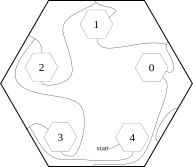
\includegraphics[width=0.6\textwidth]{power4.pdf}
  \caption{The ``power-of-two'' maze. \label{fig:power2}}
\end{figure}

And there is worse: the length of a shortest path can itself be exponential in
the size of any reasonable description of the maze. Consider for instance the
maze shown in Fig.~\ref{fig:power2}. A moment's thought will reveal that there
is a path from the north-east to the south that goes through 0. Then, there is a
path from the north to the south that enters 1, goes through 0, exits 1 and go
through 0 again. Then there is a path from the north-west that enters 2, goes
through 1, exits 2 and goes through 1 again, etc. Generalizing this construction
to an $n$-gon yields a family of recursive mazes where the only way to exit
makes an exponential number of steps in the size of the maze.

We first take one aspect of the problem off the table: out of the two possible
goals (getting out of the maze, or reaching $\oplus$ starting from $\ominus$),
only getting out is interesting. More precisely, every maze where the goal is to
reach a specific wire can be converted into another maze where the goal is to
exit. Fig.~\ref{fig:convert} shows how. Interestingly, we do not know how to
make the conversion the other way around. The obvious attempt (shown in
Fig.~\ref{fig:convert-bad}) fails, because it creates extra connections between
wires that may lead to spurious solutions. For instance, it allows to escape the
unescapable ``innocent-looking'' maze shown above.

\begin{figure}
  \centering
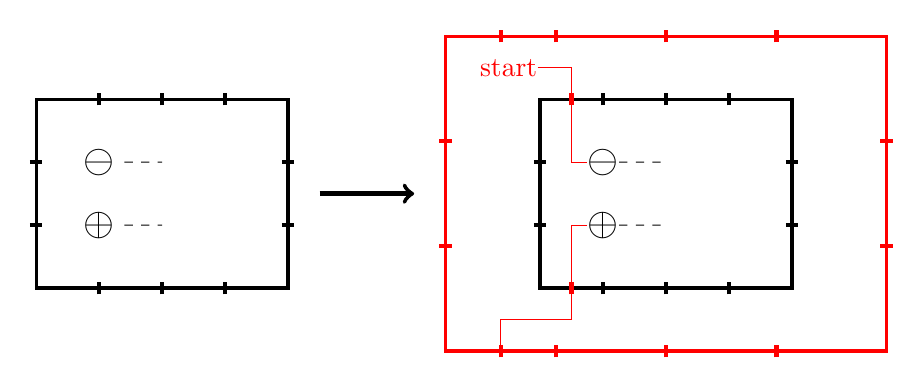
\begin{tikzpicture}[scale=0.8]
  \begin{scope}
    \node at (1, 2) (minus) {\Large $\ominus$};
    \node at (1, 1) (plus) {\Large $\oplus$};
    \draw[dashed] (plus) -- +(1, 0);
    \draw[dashed] (minus) -- +(1, 0);

    \draw[very thick] (0, 0) rectangle +(4, 3);
    \foreach \i in {1, 2} {
      \draw[ultra thick] (0, \i) +(-0.1, 0) -- +(0.1, 0);
      \draw[ultra thick] (4, \i) +(-0.1, 0) -- +(0.1, 0);
    }
    \foreach \i in {1, 2, 3} {
      \draw[ultra thick] (\i, 0) +(0, -0.1) -- +(0, 0.1);
      \draw[ultra thick] (\i, 3) +(0, -0.1) -- +(0, 0.1);
    }
  \end{scope}

  \draw[ultra thick,->] (4.5, 1.5) -- (6, 1.5);
  
  \begin{scope}[xshift=8cm]
    \draw[red, very thick] (-1.5, -1) rectangle +(7, 5);

    \node[inner sep=0] at (1, 2) (minus) {\Large $\ominus$};
    \node[inner sep=0] at (1, 1) (plus) {\Large $\oplus$};
    \draw[dashed] (plus) -- +(1, 0);
    \draw[dashed] (minus) -- +(1, 0);

    \draw[very thick] (0, 0) rectangle +(4, 3);
    \foreach \i in {1, 2} {
      \draw[ultra thick] (0, \i) +(-0.1, 0) -- +(0.1, 0);
      \draw[ultra thick] (4, \i) +(-0.1, 0) -- +(0.1, 0);
      \draw[red,ultra thick] (-1.5, 5*\i/3-1) +(-0.1, 0) -- +(0.1, 0);
      \draw[red,ultra thick] (5.5, 5*\i/3-1) +(-0.1, 0) -- +(0.1, 0);
    }
    \foreach \i in {1, 2, 3} {
      \draw[ultra thick] (\i, 0) +(0, -0.1) -- +(0, 0.1);
      \draw[ultra thick] (\i, 3) +(0, -0.1) -- +(0, 0.1);
      \draw[red,ultra thick] (7*\i/4-1.5, -1) +(0, -0.1) -- +(0, 0.1);
      \draw[red,ultra thick] (7*\i/4-1.5, 4) +(0, -0.1) -- +(0, 0.1);
    }
    \draw[red,ultra thick] (7*0.5/4-1.5, -1) +(0, -0.1) -- +(0, 0.1);
    \draw[red,ultra thick] (7*0.5/4-1.5, 4) +(0, -0.1) -- +(0, 0.1);

    \node[red,inner sep=0] at (-0.5, 3.5) (start) {start};
    \draw[red,ultra thick] (0.5, 3) +(0, -0.1) -- +(0, 0.1);
    \draw[red] (start) -| (0.5, 3); 
    \draw[red] (0.5, 3) |- (minus); 

    \draw[red,ultra thick] (0.5, 0) +(0, -0.1) -- +(0, 0.1);
    \draw[red] (plus) -| (0.5, -0.5); 
    \draw[red] (0.5, -0.5) -| (7*0.5/4-1.5, -1); 
\end{scope}
\end{tikzpicture}
\caption{\label{fig:convert} Converting a maze from ``reaching an internal
  goal'' to ``getting out''. The new red maze contains all the content of the
  original maze plus an extra recursive box that connects ``start'' to
  $\ominus$.}
\end{figure}

\begin{figure}
  \centering
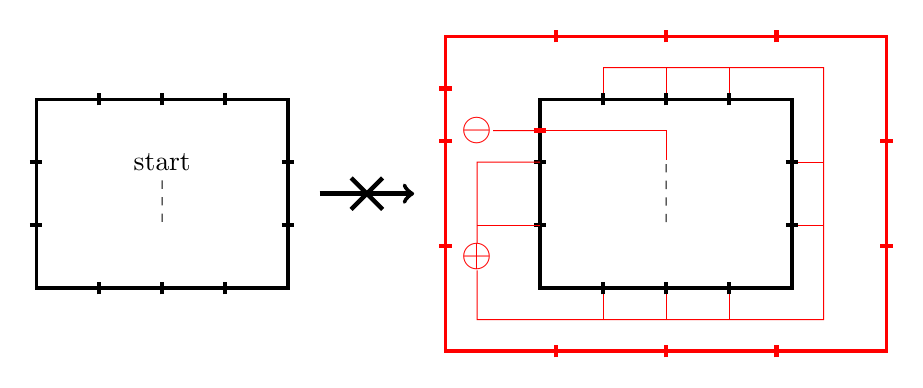
\begin{tikzpicture}[scale=0.8]
  \begin{scope}
    \node at (2, 2) (start) {start};
    \draw[dashed] (start) -- +(0, -1);
    \draw[very thick] (0, 0) rectangle +(4, 3);
    \foreach \i in {1, 2} {
      \draw[ultra thick] (0, \i) +(-0.1, 0) -- +(0.1, 0);
      \draw[ultra thick] (4, \i) +(-0.1, 0) -- +(0.1, 0);
    }
    \foreach \i in {1, 2, 3} {
      \draw[ultra thick] (\i, 0) +(0, -0.1) -- +(0, 0.1);
      \draw[ultra thick] (\i, 3) +(0, -0.1) -- +(0, 0.1);
    }
  \end{scope}

  \draw[ultra thick,->] (4.5, 1.5) -- (6, 1.5);
  \draw[ultra thick] (5, 1.75) -- (5.5, 1.25);
  \draw[ultra thick] (5.5, 1.75) -- (5, 1.25);
  
  \begin{scope}[xshift=8cm]
    \node[inner sep=0] at (2, 2) (start) {};
    \draw[dashed] (start) -- +(0, -1);
    \draw[very thick] (0, 0) rectangle +(4, 3);
    \foreach \i in {1, 2} {
      \draw[ultra thick] (0, \i) +(-0.1, 0) -- +(0.1, 0);
      \draw[red] (4, \i) -- (4.5, \i);
      \draw[ultra thick] (4, \i) +(-0.1, 0) -- +(0.1, 0);
      \draw[red,ultra thick] (-1.5, 5*\i/3-1) +(-0.1, 0) -- +(0.1, 0);
      \draw[red,ultra thick] (5.5, 5*\i/3-1) +(-0.1, 0) -- +(0.1, 0);
    }
    \draw[red,ultra thick] (-1.5, 5*2.5/3-1) +(-0.1, 0) -- +(0.1, 0);

    \foreach \i in {1, 2, 3} {
      \draw[red] (\i, 0) -- (\i, -0.5);
      \draw[ultra thick] (\i, 0) +(0, -0.1) -- +(0, 0.1);
      \draw[red] (\i, 3) -- (\i, 3.5);
      \draw[ultra thick] (\i, 3) +(0, -0.1) -- +(0, 0.1);
      \draw[red,ultra thick] (7*\i/4-1.5, -1) +(0, -0.1) -- +(0, 0.1);
      \draw[red,ultra thick] (7*\i/4-1.5, 4) +(0, -0.1) -- +(0, 0.1);
    }

    \draw[red, very thick] (-1.5, -1) rectangle +(7, 5);
    \node[red,inner sep=0] at (-1, 2.5) (minus) {\Large $\ominus$};
    \node[red,inner sep=0] at (-1, 0.5) (plus) {\Large $\oplus$};
    \draw[red,ultra thick] (0, 2.5) +(-0.1, 0) -- +(0.1, 0);
    \draw[red] (minus) -- (0, 2.5);
    \draw[red] (0, 2.5) -| (start);

    \draw[red] (1, 3.5) -- (4.5, 3.5) -- (4.5, -0.5) -- (-1, -0.5) -- (plus);
    \draw[red] (0, 2) -- (-1, 2) -- (plus);
    \draw[red] (0, 1) -- (-1, 1);
\end{scope}
\end{tikzpicture}
\caption{\label{fig:convert-bad} Trying to convert a ``getting out'' maze into a
  ``reach internal target'' maze in the obvious way does not work (it creates
  extra connections between wires).}
\end{figure}


In this article, we consider old and new algorithms to decide, in polynomial
time, if the maze can be exited or not. All these algorithms produces (in
polynomial time) a description of a solution path, even if it is of exponential
length. We compare their complexities, expressed in terms of various
characteristics of the maze: the number of wires $W$, the number of recursive
boxes $B$ and the number $E$ of possible ways to enter a recursive box (8 in the
maze on the left of Fig.~\ref{fig:simple}).

\begin{figure}[t]
  \centering
  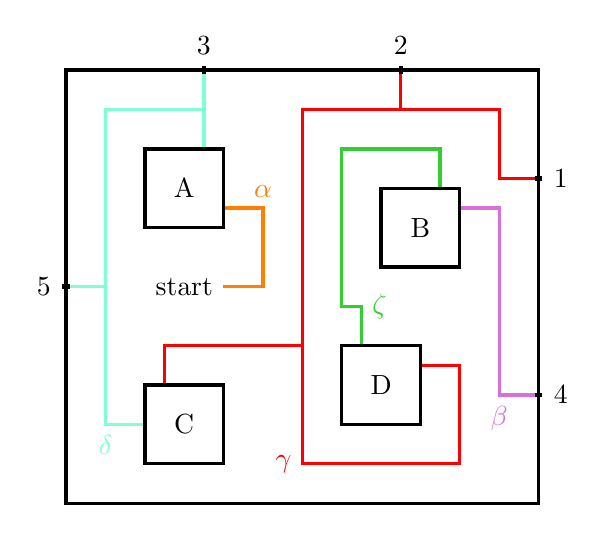
\begin{tikzpicture}[scale=0.5]
  \draw[very thick] (-1, -1) rectangle (11, 10);

  \draw[very thick, Aquamarine] (-1, 4.5) -- (0, 4.5) -- (0, 1) node[below] {$\delta$} -- (1, 1);
  \draw[very thick, Aquamarine] (0, 4.5) -- (0, 9) -- (2.5, 9) -- (2.5, 8);
  \draw[very thick, Aquamarine] (2.5, 9) -- (2.5, 10);

  \draw[very thick, Orchid] (11, 1.75) -- (10, 1.75) node[below] {$\beta$} -- (10, 6.5) -- (9, 6.5);
  \draw[very thick, LimeGreen] (8.5, 7) -- (8.5, 8) -- (6, 8) -- (6, 4) -- (6.5, 4) node[right] {$\zeta$} -- (6.5, 3);

  \draw[very thick, red] (1.5, 2) -- (1.5, 3) -- (5, 3) -- (5, 9) -- (10, 9) -- (10, 7.25) -- (11, 7.25);
  \draw[very thick, red] (7.5, 9) -- (7.5, 10);
  \draw[very thick, red] (5, 3) -- (5, 0) node[left] {$\gamma$} -- (9, 0) -- (9, 2.5) -- (8, 2.5);

  \node at (2, 4.5) (start) {start};
  \draw[very thick, orange] (start) -- (4, 4.5) -- (4, 6.5) node[above] {$\alpha$} -- (3, 6.5);

  \draw[very thick] (1, 0) rectangle node {C} +(2, 2);
  \draw[very thick] (1, 6) rectangle node {A} +(2, 2);
  \draw[very thick] (6, 1) rectangle node {D} +(2, 2);
  \draw[very thick] (7, 5) rectangle node {B} +(2, 2);

  \draw[ultra thick] (-1, 4.5) +(-0.1, 0) node[left] {5} -- +(0.1, 0);
  \draw[ultra thick] (2.5, 10) +(0, -0.1) -- +(0, 0.1) node[above] {3};
  \draw[ultra thick] (7.5, 10) +(0, -0.1) -- +(0, 0.1) node[above] {2};
  \draw[ultra thick] (11, 1.75) +(-0.1, 0) -- +(0.1, 0) node[right] {4};
  \draw[ultra thick] (11, 7.25) +(-0.1, 0) -- +(0.1, 0) node[right] {1};
\end{tikzpicture}
\hfill
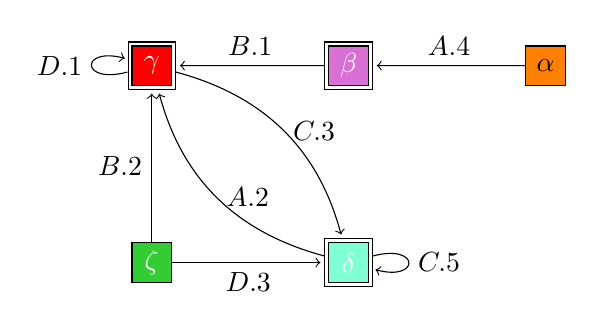
\begin{tikzpicture}[scale=1.25]
  \node[extra box] at (0, 2) (R) {};
  \node[wire,fill=red,text=white] at (0, 2) {$\gamma$};
  
  \node[wire,fill=LimeGreen,text=white] at (0, 0) (G) {$\zeta$};
  \node[wire, fill=orange] at (4, 2) (start) {$\alpha$};
  
  \node[extra box] at (2, 0) (B) {};
  \node[extra box] at (2, 2) (K) {};
  \node[wire,fill=Aquamarine,text=white] at (2, 0) {$\delta$};
  \node[wire,fill=Orchid,text=white] at (2, 2) {$\beta$};
  
    \draw (start) edge[->] node[above] {$A.4$} (K);

    \draw (K) edge[->] node[above] {$B.1$} (R);

    \draw (B) edge[->, "$C.5$", loop right] (C);
    \draw (B) edge[->, bend left] node[right] {$A.2$} (R);
    \draw (G) edge[->] node[below] {$D.3$} (B);

    \draw (R) edge[->, "$D.1$", loop left] (R);
    \draw (G) edge[->] node[left] {$B.2$} (R);
    \draw (R) edge[->, bend left] node[right] {$C.3$} (B);
  \end{tikzpicture}
  
  \caption{A simple maze of our own design (left) and its ``dual'' representation (right). Wires with a double-box are ``accepting'' (connected to an outer IO pin). \label{fig:simple}}
\end{figure}

After presenting some context, we review in section~\ref{sec:shelf} the
classical technique that decides emptiness of the context-free language
associated to a deterministic pushdown automaton built from the description of
the maze. It runs in time $\bigO{W^2EB}$. In section~\ref{sec:modelchecking}, we
review improved algorithms to decide reachability of arbitrary states in
pushdown automata, that yield a faster decision procedure with complexity
$\bigO{\mathcal{W}^3}$. Finally, in section~\ref{sec:us} we discuss a new
algorithmic technique to compute equivalence classes of wires inside a recursive
maze. In section~\ref{sec:implem} we discuss the efficient implementation of
this procedure, and show a version that terminates in time
$\bigO{WB + E \alpha(W)}$, where $\alpha$ is the inverse-Ackermann function,
improving the state of the art. We discuss how to bring this down to
$\bigO{E \log E}$, but this seems to either require: a) cheating, or b)
randomization. Lastly, in section~\ref{sec:arg}, we discuss how to actually
construct an exit path (this was the whole point of the paper, isn't it?).

``Solving'' recursive mazes in linear time, e.g. $\bigO{W + B + E}$ is left as
an intriguing open problem.

\section{Topological representation of recursive mazes}

A recursive maze has several parameters: the number $B$ of recursive boxes (from
2 to 8 in the given examples), the number of output pins, the number $W$ of
wires. As a convention, inner boxes are identified by capital letters (A, B, C,
...), outer IO pins are referenced by numbers and wires are referenced by Greek
letters. An inner IO pin (on a recursive box) is referenced by the identifier of
the box and that of the pin. For example, on Fig.~\ref{fig:infinite} (left),
``1'' is connected to ``A.6'' and ``C.3''.  An \emph{endpoint} is either an
outer pin, or an inner pin. A wire connects a set of endpoints. For instance,
the wires of the simple maze shown on the left of Fig.~\ref{fig:simple} are:
\[
  \{\texttt{start}, A.4\}, 
  \{4, B.1\}, 
  \{1, 2, C.3, D.1\},
  \{3, 5, A.2, C.5\}, 
  \{D.2, B.2\}
\]

This completely represents the maze, and can easily be encoded as a text
file. The size of this text file is a good measure of the size of the maze. Note
that a recursive maze is therefore a hypergraph whose vertices are the
endpoints.  It even seems legitimate to consider this as ``the'' abstract
description of the maze. Note that in principle each endpoint must appear in at
most one wire, and each outer IO pin must appear in exactly one wire for
the maze to be well-formed. This implies that $E \leq BP$ and $W \leq P$.

An alternate, ``dual'' description is also useful (Fig.~\ref{fig:simple},
right): it is a directed graph whose nodes are the wires of the maze, and where
there is a directed edge $\alpha \xrightarrow{X.i} \beta$ if it is possible to
go from wire $\alpha$ to wire $\beta$ by entering the recursive box labelled $X$
using its pin labelled $i$. As before, $E$ denotes the number of edges of this
graph. The dual representation graph can be assembled in essentially linear time
from the previous ``hypergraph'' representation:
\begin{itemize}
\item First, associate each outer pin to the wire that contains it.
\item Initialize an empty directed graph $G$ on the wires.
\item Then, for each wire $\phi$, do:
  \begin{itemize}
  \item For each inner pin $X.i$ in $\phi$, add an edge labelled by $X.i$ from
    $\phi$ to the wire containing the outer pin $i$ (if it does not already
    exist).
  \end{itemize}
\end{itemize}

It follows from the well-formedness conditions that all edge labels are distinct
in the dual representation graph. The original ``hypergraph'' representation can
be reassembled from the dual representation graph, under the assumption that the
initial location (\texttt{start}) is always incident to the wire $\alpha$. An
edge $\alpha \xrightarrow{X.i} \beta$ means that the outer IO pin $i$ belongs to
wire $\beta$, and that $X.i$ belongs to wire $\alpha$. By convention, the
starting point (\texttt{start}) belongs to wire $\alpha$.

% non-minimality
Nothing prevent several outer IO pins to belong to the same wire. In the simple
maze of Fig.~\ref{fig:simple}, pins $(1, 2)$ and $(3, 5)$ are connected. But is
this really necessary? When two outer IO pins belong to the same wire, couldn't
we remove one of them (and redirect connections to the other one)? To answer
this question, take the dual representation graph and \emph{erase} all pin
information:

\begin{center}
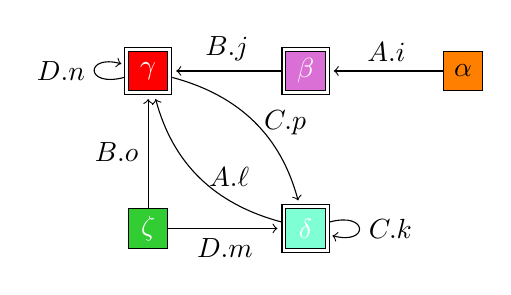
\begin{tikzpicture}[scale=1]
  \node[extra box] at (0, 2) (R) {};
  \node[wire,fill=red,text=white] at (0, 2) {$\gamma$};
  
  \node[wire,fill=LimeGreen,text=white] at (0, 0) (G) {$\zeta$};
  \node[wire, fill=orange] at (4, 2) (start) {$\alpha$};
  
  \node[extra box] at (2, 0) (B) {};
  \node[extra box] at (2, 2) (K) {};
  \node[wire,fill=Aquamarine,text=white] at (2, 0) {$\delta$};
  \node[wire,fill=Orchid,text=white] at (2, 2) {$\beta$};
  
    \draw (start) edge[->] node[above] {$A.i$} (K);

    \draw (K) edge[->] node[above] {$B.j$} (R);

    \draw (B) edge[->, loop right] node[right] {$C.k$} ();
    \draw (B) edge[->, bend left] node[right] {$A.\ell$} (R);
    \draw (G) edge[->] node[below] {$D.m$} (B);

    \draw (R) edge[->, loop left] node[left] {$D.n$} (R);
    \draw (G) edge[->] node[left] {$B.o$} (R);
    \draw (R) edge[->, bend left] node[right] {$C.p$} (B);
  \end{tikzpicture}
\end{center}

Then formulate the constraints:
\begin{itemize}
\item Different wires are not ``inadvertently'' connected to the same outer IO
  pin. This means that $\{i\}, \{j, n, o\}$, $\{p, m, k\}$ must be pairwise disjoint.
\item Endpoints appear in a single wire. This means that inside the following sets, values are all different: $\{i, \ell\}, \{j, o\}, \{p, k\}$ and $\{n, m\}$.
\end{itemize}
The problem of assigning integer values in $\{1, \dots, N\}$, to the variables,
for the smallest possible $N$, can be seen as a variant of the
\textsc{Colorability} problem, but it is an easy one. A simple algorithm will
satisfy the constraints using the minimum possible number of values: first
compute a ``local'' assignment of values to the unknowns for each disjoint
subset in isolation ; then form a global assignment by ``shifting'' values
already used in previous subsets.  For instance, in the example above,
satisfying the inequality constraints inside each disjoint subset leads to:
\begin{align*}
  i &\leadsto 1 \\
  j, n, o &\leadsto (1, 1, 2) \\
  p, m, k &\leadsto (1, 1, 2)
\end{align*}
Then assembling all disjoint subsets leads to:
\[
  (i), (j, n, o), (p,m,k) \leadsto (1), (2,2,3), (4,4,5)
\]
Therefore, the simple maze discussed above cannot be simplified further: at
least 5 outer IO pins are necessary (and sufficient). Let the disjoint subsets
be $A_1, \dots, A_k$, and the all-different ones be $B_1, \dots, B_\ell$ (note
that the $B_j$'s are also disjoint, because they correspond to different boxes).
Then inside a disjoint subset $A_i$, the variables in $A_i \cap B_j$ must be all
different, for each $j$. Therefore, $\min_j |A_i \cap B_j|$ values are necessary
(and sufficient) for $A_i$.

Let us next look at the small maze on the right of Fig.~\ref{fig:jpwolf}. We
number its pins from 0 to f clockwise (0,1,2,3 at the north, 4, 5, 6, 7 on the
east side, 8,9,a,b at the south and c,d,e,f at on the west side). Pin 1 is
clearly a decoy: nothing is connected to either $A.1$, $B.1$ or $C.1$. Next,
pins 0, $e$ and $f$ belong to the same wire, but one of them is redundant. There
are connections to $A.0, B.0, C.0, C.e, A.f$ and $B.f$, therefore ``merging''
$e$ and $f$ is possible without creating extra connections. We assume that these
extra pins are present for aesthetic reasons.

\section{Recursive mazes as pushdown automata}

Navigating recursive mazes in one's head is difficult because it is necessary to
keep track of all the boxes that have been entered (and by what pin).

Suppose a sequence of instructions is given by the player to some kind of game
engine. These instructions can be of three kinds: ``from the current location,
enter box $X$ using its pin $i$'' (encoded as $X.i$) or ``from the current
location, leave the current box $X$ through the outer pin $i$'' (encoded as $\overline{X.i}$) and finally ``I have solved the problem'' (\texttt{done}). For
instance, this is a sequence of instructions for the the simple maze of
Fig.~\ref{fig:simple} (that presumably exits):
\[
  A.4; B.1; \overline{B.2}; D.3; C.5; \overline{C.3}; \overline{D.1}; \overline{A.2}; \texttt{done}
\]
We note that $\overline{X.i}$ could be more compactly encoded as just ``$i$''
(we do not need to know that we are inside box $X$ to just take the
exit). However, this more verbose encoding enables us to define the
\emph{mirror} operation on instructions (also denoted with an overline):
$\overline{X.i}$ is the mirror of $X.i$, and vice-versa so that
$\overline{\overline{X.i}} = X.i$. Applying a (legal) instruction then its
mirror is a no-op (the mirror cancels the effect of the first instruction).
Lists of instructions can also be mirrored, by mirroring each instruction
individually and reversing their order:
$\overline{A.4; B.1; \overline{B.2}} = B.2; \overline{B.1};
\overline{A.4}$. Applying a sequence of legal instruction then its mirror is a
no-op.

There is a way to efficiently check if a sequence of instruction is valid,
i.e. if the desired moves are actually feasible. The validity of a move depend
on the last box that was entered (for instance $\overline{A.2}$ is valid inside
A but not inside B, C and D). So it is required to track the current box, as
boxes are entered and exited. The analogy with the call stack of a recursive
function is quite obvious. This also strongly suggests some kind of
stack-augmented automaton. This brilliant observation has certainly been made
many times, by many people independently (including us), but a notorious and
early statement is due to Peter Shor (of quantum polynomial factoring fame) in
2012, as a comment to a question on
\href{https://cstheory.stackexchange.com/questions/11024/decidability-of-fractal-maze}{StackExchange}). He
writes:
\begin{quote}
  \it 
  Can't you represent any fractal maze as a pushdown automaton, where the stack
  corresponds to the sequence of submazes that you're in? Then the solubility
  question would turn into the emptiness problem for context-free languages,
  which is decidable.
\end{quote}

Making this intuition precise is easier with the dual representation graph of
recursive mazes. We assume that there is an initial wire (denoted as $\alpha$)
where the player starts. The position of the player consists of a current wire
and a stack of entered boxes. We write such a position as ``wire | stack'' or
``$\frac{\text{wire}}{\text{stack}}$''. The stack is initialized with the
identifier of the ``main'' box that contains everything, which is denoted as
$\bot$. Moving between wires pushes box identifiers on the stack (when a box is
entered), or pops them (when a box is left). Entering box $X$ is always possible
(if there is a wire leading to it of course), but exiting box $X$ only makes
sense if we are currently inside it.  The possible transitions from a given
state are thus entirely determined by the top of the stack. If there is an edge
$\phi \xrightarrow{X.i} \psi$ in the dual representation of the maze, then the
player may move between positions $\phi | S$ and $\psi | X ; S$ (both ways) by
issuing $X.i$ or $\overline{X.i}$.

We can therefore describe a deterministic pushdown automaton (DPDA) for the
maze, that accepts by empty stack. Suppose the set of outer pins is
$\mathcal{P}$ (think $1, \dots, n$), the set of recursive boxes is $\mathcal{B}$
(think $\bot, A, B, C, \dots$) and the set of wires is $\mathcal{W}$ (think $\alpha, \beta,
\dots$). % Denote by $\rho : \mathcal{P} \rightarrow \mathcal{W}$ the function
% that maps an outer pin $i$ to the wire that contains $i$.
\begin{itemize}
\item The set of \emph{states} of the DPDA is $Q := \mathcal{W} \cup \{\texttt{goal} \}$.
\item The \emph{input alphabet} is $\Sigma := \mathcal{B} \times \mathcal{P} \cup \overline{\mathcal{B} \times \mathcal{P}}$.
\item The \emph{stack alphabet} is $\Lambda := \mathcal{B}$.
\item The \emph{start state} is a designated wire $\alpha \in \mathcal{W}$ (part of the specification of the maze).
\item The \emph{initial stack symbol} is $\bot$ (the global box).
\item The \emph{transition function}
  $f : Q \times \Sigma \times \Lambda \rightarrow Q \times \Lambda^*$ is defined
  as follows. For every edge $\phi \xrightarrow{X.i} \psi$ in the
  dual representation graph and for any box $Y \in \mathcal{B}$,
  $f(\phi, X.i, Y) = (\psi, XY)$ and
  $f(\psi, \overline{X.i}, X) = (\phi, \emptyset)$. If the goal is to exit the
  maze, additionally set $f(\omega, \texttt{done}, \bot) = (\texttt{goal}, \emptyset)$
  for all wires $\omega$ adjacent to an outer IO pin. If the goal is to reach a
  specific wire $\omega$, set
  $f(\oplus, \texttt{done}, \bot) = (\texttt{goal}, \emptyset)$.
\end{itemize}

This pushdown automaton accepts all sequences of instructions that solve the
maze. For instance, the following is a legal sequence of transitions in the
simple maze of Fig.~\ref{fig:simple} (that exits the maze):

\begin{center}
\noindent\scalebox{0.925}{%
$\displaystyle
  \frac{\alpha}{\bot}
  \xrightarrow{A.4} \frac{\beta  }{ A \bot}
  \xrightarrow{B.1} \frac{\gamma }{ BA \bot}
  \xrightarrow{\overline{B.2}}   \frac{\zeta  }{ A \bot}
  \xrightarrow{D.3} \frac{\delta }{ DA \bot}
  \xrightarrow{C.5} \frac{\delta }{ CDA \bot}
  \xrightarrow{\overline{C.3}}   \frac{\gamma }{ DA \bot}
  \xrightarrow{\overline{D.1}}   \frac{\gamma }{ A \bot}
  \xrightarrow{\overline{A.2}}   \frac{\delta }{ \bot}
  \xrightarrow{\texttt{done}}    \frac{\scriptstyle \texttt{goal}}{}
$}%
\end{center}

As a consequence, the sequences of instructions that exit the maze form a
(deterministic) context-free language. We note that there are off-the-shelf
software libraries to test reachability of configurations in pushdown automata
such as \textsf{Moped}~\cite{DBLP:phd/dnb/Schwoon02} or
\textsf{PDAAAL}~\cite{DBLP:conf/atva/JensenSSS22} (just to mention a few) that
can therefore be used to solve recursive mazes.

\section{Construction of mazes with an exit path of a prescribed length}

The dual representation of recursive mazes can be useful as a design tool. For
instance, we highlight the conception of mazes where the exit path has a
prescribed length. This length must be odd (because each entered box must be
exited, and there is \texttt{done} at the end).  For instance, suppose we would
like to build a maze with a path of length 1337 (a random \texttt{leet}
value). We start from a a \emph{twisted addition chain} for 1335:
\begin{align*}
  5 &= 1 + (1+1) + (1+1) \\
  19 &= 1 + (5+1) + (5+1) + (5+1) \\
  101 &= 1 + (19+1) + (19+1) + (19+1) + (19+1) + (19+1) \\
  307 &= 1 + (101+1) + (101+1)+ (101+1) \\
  1335 &= 1 + (101+1) + (307+1) + (307+1) + (307+1) + (307+1)
\end{align*}
And we build the following graph (pins were assigned using the algorithm outlined above):

\begin{center}
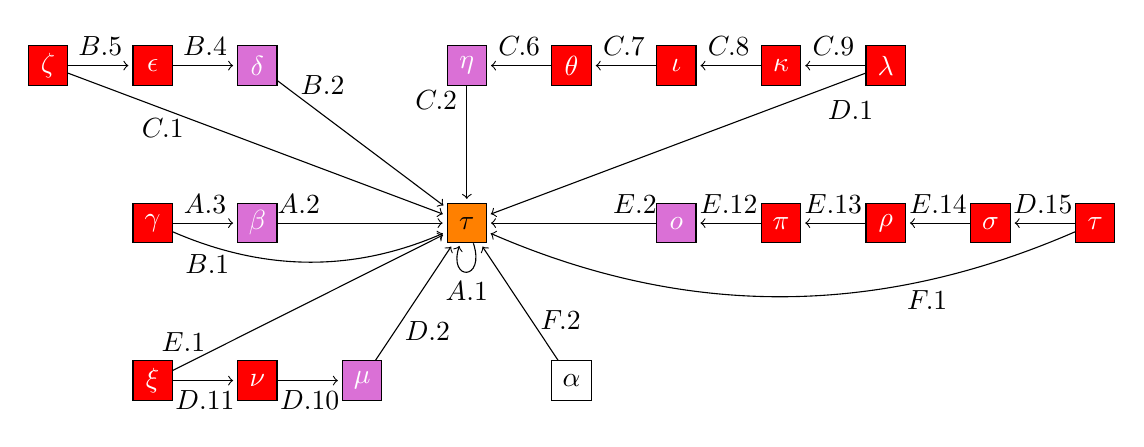
\begin{tikzpicture}[xscale=1.33]
  \node[wire,fill=orange] at (0, 0) (alpha) {$\tau$};
  \draw (alpha) edge[loop below] node[below] {$A.1$} ();
  
%  \node[extra box] at (1, -2) (upsilon) {};
  \node[wire, draw] at (1, -2) (upsilon) {$\alpha$};
  \draw (upsilon) edge[->] node[near start, above right=-1mm] {$F.2$} (alpha);

  % chain for A/B 2
  \node[wire,fill=Orchid,text=white] at (-2, 0) (beta) {$\beta$};
  \node[wire,fill=red,text=white] at (-3, 0) (gamma) {$\gamma$};
  \draw (beta) edge[->] node[above,very near start] {$A.2$} (alpha);
  \draw (gamma) edge[->] node[above] {$A.3$} (beta);
  \draw (gamma) edge[->, bend right] node[below, very near start] {$B.1$} (alpha);
  
  % chain for B/C 3
  \node[wire,fill=Orchid,text=white] at (-2, 2) (delta) {$\delta$};
  \node[wire,fill=red,text=white] at (-3, 2) (epsilon) {$\epsilon$};
  \node[wire,fill=red,text=white] at (-4, 2) (zeta) {$\zeta$};
  \draw (delta) edge[->] node[above right=-1mm,very near start] {$B.2$} (alpha);
  \draw (epsilon) edge[->] node[above] {$B.4$} (delta);
  \draw (zeta) edge[->] node[above] {$B.5$} (epsilon);
  \draw (zeta) edge[->] node[below,near start] {$C.1$} (alpha);

  % chain for C/D 5
  \node[wire,fill=Orchid,text=white] at (0, 2) (eta) {$\eta$};
  \node[wire,fill=red,text=white] at (1, 2) (theta) {$\theta$};
  \node[wire,fill=red,text=white] at (2, 2) (iota) {$\iota$};
  \node[wire,fill=red,text=white] at (3, 2) (kappa) {$\kappa$};
  \node[wire,fill=red,text=white] at (4, 2) (lambda) {$\lambda$};
  \draw (lambda) edge[->] node[above] {$C.9$} (kappa);
  \draw (kappa) edge[->]  node[above] {$C.8$} (iota);
  \draw (iota) edge[->]   node[above] {$C.7$} (theta);
  \draw (theta) edge[->]  node[above] {$C.6$} (eta);
  \draw (eta) edge[->]    node[left,very near start] {$C.2$} (alpha);
  \draw (lambda) edge[->] node[below right=0mm, very near start] {$D.1$} (alpha);

  % chain for D/E 3
  \node[wire,fill=Orchid,text=white] at (-1, -2) (mu) {$\mu$};
  \node[wire,fill=red,text=white] at (-2, -2) (nu) {$\nu$};
  \node[wire,fill=red,text=white] at (-3, -2) (xi) {$\xi$};
  \draw (xi) edge[->] node[below] {$D.11$} (nu);
  \draw (nu) edge[->] node[below] {$D.10$} (mu);
  \draw (mu) edge[->] node[right=0mm,near start] {$D.2$} (alpha);
  \draw (xi) edge[->] node[above left=-1mm, very near start] {$E.1$} (alpha);

  % chain for D/E/F 4
  \node[wire,fill=Orchid,text=white] at (2, 0) (omicron) {$o$};
  \node[wire,fill=red,text=white] at (3, 0) (pi) {$\pi$};
  \node[wire,fill=red,text=white] at (4, 0) (rho) {$\rho$};
  \node[wire,fill=red,text=white] at (5, 0) (sigma) {$\sigma$};
  \node[wire,fill=red,text=white] at (6, 0) (tau) {$\tau$};

  \draw (omicron) edge[->] node[above,very near start] {$E.2$} (alpha);
  \draw (pi) edge[->] node[above] {$E.12$} (omicron);
  \draw (rho) edge[->] node[above] {$E.13$} (pi);
  \draw (sigma) edge[->] node[above] {$E.14$} (rho);
  \draw (tau) edge[->] node[above] {$D.15$} (sigma);
  \draw (tau) edge[->, bend left] node[below=0mm, near start] {$F.1$} (alpha);
\end{tikzpicture}
\end{center}

The resulting maze has 15 pins, 6 recursive boxes and 20 wires. An exit path is provided by:
\begin{align*}
  \mathcal{P}_5    &:= \overline{B.1}; A.3; A.2; \overline{A.1}; \overline{A.1}  \\   % pop B
  \mathcal{P}_{19}  &:= \overline{C.1}; B.5; B.4;  B.2; \left(\mathcal{P}_5\right)^3 \\  % pop C
  \mathcal{P}_{101} &:= \overline{D.1}; C.9; C.8; C.7; C.6; C.2; \left(\mathcal{P}_{19}\right)^5  \\ %pop D
  \mathcal{P}_{307} &:= \overline{E.1}; D.11; D.10; D.2; \left(\mathcal{P}_{101}\right)^3  \\ % pop E
  \mathcal{P}_{1335}&:= \overline{F.1 }; D.15; E.14; E.13; E.12; E.2; \left(\mathcal{P}_{307}\right)^4; \left(\mathcal{P}_{101}\right) \\ % pop F
  \mathcal{P}_{1337}&:= F.2; \left(\mathcal{P}_{1335}\right); \texttt{done}
\end{align*}
The point is that the sequence of instruction $\mathcal{P}_5$ takes the player
from wire $\tau$ to wire $\tau$ but exits box $B$. $\mathcal{P}_{19}$ does the
same with box $C$, $\mathcal{P}_{101}$ with box $D$, etc.  It is left to the
reader to check that $\mathcal{P}_x$ has length $x$. We also hope that, at this
point, the role of the ``twisted addition chains'' has become clear. A Twisted
addition chain is a sequence of equalities of the kind
$a_{i+1} = [\text{sum of $k$ previous $a_i$'s}] + (k+1)$, starting with
$a_0 = 1$. The number of recursive boxes is one plus the number of steps of the twisted
addition chain. The number of wires is two plus the total number of occurrences
of all constants in right-hand sides of the twisted addition chain, and pins =
wires + 1 - boxes.

The alternative twisted addition chain:
\begin{align*}
  3 &= 1 + (1+1) \\
  9 &= 1 + (3+1) + (3+1) \\
  21 &= 1 + (9+1) + (9+1) \\
  45 &= 1 + (21+1) + (21+1) \\
  93 &= 1 + (45+1) + (45+1) \\
  189 &= 1 + (93+1) + (93+1) \\
  571 &= 1 + (189+1) + (189+1) + (189+1) \\
  1335 &= 1 + (189+1) + (571+1) + (571+1)
\end{align*}
leads to a different maze with 9 recursive boxes, 11 pins and only 19
wires.

Using this strategy with a sequence of ``doubling plus three'' steps only yields
a variant of the ``power-of-two'' maze shown in Fig.~\ref{fig:power2}. Using a twisted
addition chain with $k$ steps of the kind $a_{i+1} = 2a_i + 3$ yields a maze
with $1+k$ boxes, $2+2k$ wires and $2+k$ IO pins. The exit path has length
$3 \cdot 2^k - 3$. This shows that the length of the exit path can be
exponential in any of the relevant quantities. 

As a side note, there is a rich theory of normal addition chains
(see~\cite{Knuth}), and we believe that the twisted ones beg for the same level
of attention.

\section{Languages associated to recursive mazes}

A context-free language can be associated to each recursive maze, but what about
the converse? Is there a recursive maze that can be exited by any syntactically
correct Python program? In this section we take a first step toward
characterizing the class of context-free languages corresponding to recursive
mazes.

Let $\mathcal{L}$ be the (context-free) language accepted by a recursive
maze. We first introduce an \emph{erasure homomorphism} $h$ such that
$h(X.i) = X$, $h(\overline{X.i}) = \overline{X}$ and
$h(\texttt{done}) = \epsilon$ (the empty string).

The $k$-\emph{Dyck} language contains all words that are well-parenthesized
using $k$ types of parentheses. For instance, \verb|([[]{}](){()})[]| $\in$
3-Dyck. In a recursive maze, each recursive box that is entered must be
exited. In a valid sequence of instruction there is a therefore properly nested
matching between ``\emph{calls}'' (entering a box) and ``\emph{returns}''
(exiting a box).  In other term, if the maze has $B$ recursive boxes
$\mathcal{B} = \{X_1, \dots, X_B\}$, then $h(\mathcal{L})$ is a contained in the
Dyck language with $B$ pairs of delimiters
$(X_1, \overline{X_1}), \dots, (X_B, \overline{X_B})$. For instance, the erasure
homomorphism sends the solution of the simple maze of Fig.~\ref{fig:simple}:
\[
  h(A.4; B.1; \overline{B.2}; D.3; C.5; \overline{C.3}; \overline{D.1}; \overline{A.2}; \texttt{done}) = ( [] \{ \langle \rangle \} )
\]


Another way of formulating the same observation is that $\mathcal{L}$ is a
\emph{regular nested words language}~\cite{10.1145/1516512.1516518}. The
pushdown automaton that accepts $\mathcal{L}$ is indeed a \emph{visibly pushdown
  automaton} (it always pushes or pops when presented with a given input symbol,
regardless of its internal state). A moment's thought reveals that $\mathcal{L}$
is in fact a (rooted) regular nested words language without internal symbol (the
construction in a sentence: entering a box is a ``call'' with a nesting edge
labelled by the box to the exit/return instruction). This already implies that
the \textsf{OpenNWA} library~\cite{10.1007/978-3-642-31424-7_47} can be used to
find a (shortest) exit path in a recursive maze.

Any Dyck language can be accepted by a recursive maze, as illustrated below for 3-Dyck:
\begin{center}
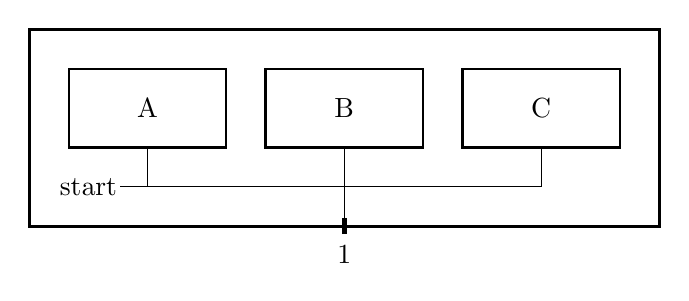
\begin{tikzpicture}[scale=0.5]
  \draw[very thick] (0, 0) rectangle +(16, 5);
%  \draw (-0.1, 1.5) -- (2, 1.5) node[right] {\tt (};
%  \draw (4, 1.5) node[left] {\tt )} -- (6.1, 1.5);

  \draw[thick] (1, 2) rectangle node {A} +(4, 2);
  \draw[thick] (6, 2) rectangle node {B} +(4, 2);
  \draw[thick] (11, 2) rectangle node {C} +(4, 2);
  \node[inner sep=1pt] at (1.5, 1) (start) {start};
  \draw (start) -- (13, 1);
  \draw (3, 2) -- (3, 1);
  \draw (8, 2) -- (8, 0);
  \draw (13, 2) -- (13, 1);
  \draw[ultra thick] (8, -0.2) -- +(0, 0.4) node[below=2mm] {1};
\end{tikzpicture}
\end{center}


So, $h(\mathcal{L})$ is a subset of a Dyck language, but not any subset: it is
contained in a \emph{regular} language derived from the maze. Imagine that the
dual representation graph is a finite automaton, in which the states
corresponding to wires connected to an outer IO pin are accepting. Then for each
edge add a ``mirror'' edge with the mirror instruction and keep only the box
label, erasing the pin label on instructions. For instance, with the simple
recursive maze of Fig.~\ref{fig:simple}:
\begin{center}
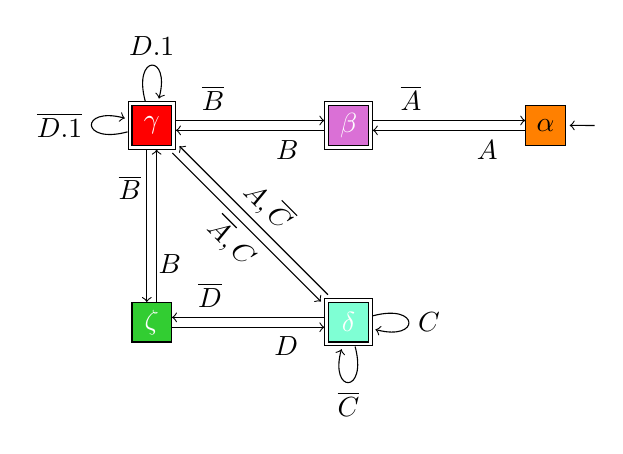
\begin{tikzpicture}[scale=1.25]
  \node[extra box] at (0, 2) (R) {};
  \node[wire,fill=red,text=white] at (0, 2) {$\gamma$};
  \node[wire,fill=LimeGreen,text=white] at (0, 0) (G) {$\zeta$};
  
  \node[extra box] at (2, 0) (B) {};
  \node[wire,fill=Aquamarine,text=white] at (2, 0) {$\delta$};

  \node[extra box] at (2, 2) (K) {};
  \node[wire,fill=Orchid,text=white] at (2, 2) {$\beta$};

  \node[wire, fill=orange] at (4, 2) (start) {$\alpha$};
  \draw (4.5, 2) edge[->] (start);

  
  \draw[<-] ($(start.west)!-0.5mm!90:(K.east)$) -- node[above, near end] {$\overline{A}$} ($(K.east)!0.5mm!90:(start.west)$);
  \draw[->] ($(start.west)!0.5mm!90:(K.east)$) -- node[below, near start] {$A$} ($(K.east)!-0.5mm!90:(start.west)$);

  %\draw (K) edge[->] node[above] {$B.1$} (R);
  \draw[<-] ($(K.west)!-0.5mm!90:(R.east)$) -- node[above, near end] {$\overline{B}$} ($(R.east)!0.5mm!90:(K.west)$);
  \draw[->] ($(K.west)!0.5mm!90:(R.east)$) -- node[below, near start] {$B$} ($(R.east)!-0.5mm!90:(K.west)$);

  
  \draw (B) edge[->, loop right] node[right] {$C$} ();
  \draw (B) edge[->, loop below] node[below] {$\overline{C}$} ();
  
%  \draw (B) edge[->, bend left] node[right] {$A.2$} (R);
%  \draw (R) edge[->, bend left] node[right] {$C.3$} (B);
  \draw[->] ($(B.north west)!-0.5mm!90:(R.south east)$) -- node[above=-0.5mm, sloped] {$A, \overline{C}$} ($(R.south east)!0.5mm!90:(B.north west)$);
  \draw[<-] ($(B.north west)!0.5mm!90:(R.south east)$) -- node[below=-0.5mm, sloped] {$\overline{A}, C$} ($(R.south east)!-0.5mm!90:(B.north west)$);

  
  % \draw (G) edge[->] node[below] {$D.3$} (B);
  \draw[->] ($(B.west)!-0.5mm!90:(G.east)$) -- node[above, near end] {$\overline{D}$} ($(G.east)!0.5mm!90:(B.west)$);
  \draw[<-] ($(B.west)!0.5mm!90:(G.east)$) -- node[below, near start] {$D$} ($(G.east)!-0.5mm!90:(B.west)$);
  
  \draw (R) edge[->, loop above] node[above] {$D.1$} ();
  \draw (R) edge[->, loop left] node[left] {$\overline{D.1}$} ();

%  \draw (G) edge[->] node[left] {$B.2$} (R);
  \draw[<-] ($(G.north)!0.5mm!90:(R.south)$) -- node[left=-0.5mm, near end] {$\overline{B}$} ($(R.south)!-0.5mm!90:(G.north)$);
  \draw[->] ($(G.north)!-0.5mm!90:(R.south)$) -- node[right=-1mm, near start] {$B$} ($(R.south)!0.5mm!90:(G.north)$);
\end{tikzpicture}
\end{center}

This non-deterministic finite automaton ``statically'' describes possible moves
in the recursive maze, ignoring the stack and the history of the computation. In
this example, it expresses that from wire $\beta$ it is possible to enter box
$B$ to reach wire $\gamma$, and that you cannot enter box $C$ from wire $\zeta$.

Denote by $R$ the regular language it accepts. Any valid sequence of instruction
that exits the maze belong to $R$ (but the converse is not true). In the end, we
find that $h(\mathcal{L}) \subseteq D \cap R$, where $D$ is the Dyck language
with $B$ delimiters and $R$ is the regular language defined above. A moment's
thought will reveal that this inclusion is in fact an equality, and yield:

\medskip
\begin{theorem}[informal]
  Let $\mathcal{L}$ be the language of all sequences of instructions that exit a
  recursive maze. Then $h(\mathcal{L})$ is precisely the intersection of the
  $B$-Dyck language with $R$, the regular language derived from the
  ``undirected'' version of the dual representation graph of the maze.
\end{theorem}

By the Chomsky-Schützenberger representation theorem~\cite{CHOMSKY1959118},
\emph{any} context-free language can be obtained by applying a homomorphism to
the intersection of a Dyck language and a regular language. This opens up the
possibility that applying a homomorphism to $\mathcal{L}$ may yield a large
class of context-free languages.

However, there is a severe restriction. The regular language in the intersection
must be such that the graph describing the associated finite automaton is
``undirected'' (see~\cite{DBLP:journals/acta/KutribMS22} for more results on
this kind of automata---they are said to be ``dual and connected''
in~\cite{STEINBERG2002341}). This highlight a nasty ``feature'' of recursive
mazes: all moves are reversible. Mistakes can be undone without having to hit
CTRL+Z, just by entering an appropriate instruction (exit the box that has just
been entered, or re-enter the box that has just been left).

In a valid sequence of instructions, it is possible to insert anywhere an
arbitrarily long sequence of arbitrary (legal) moves, and then ``undo'' them to
return to the same position while leaving the stack unchanged. This shows that
even very simple \emph{regular} languages (recognized by a deterministic finite
automaton) such as $a^* b^*$ cannot be obtained by applying a homomorphism to
$\mathcal{L}$. Indeed, suppose it could: the homomorphism sends some
instructions to $a$ and some others to $b$. Start from a valid sequence of
instruction that emits a word in the language (say $aaaabb$). Then ``undo'' it
and replay it. This yields another valid sequence of instructions that emits
``$aaaabb\,[$some stuff$]\,aaaabb$'', and this does not belong to $a^* b^*$.

\emph{Irreversible progress} is banned from maze-associated languages. 

We see a striking analogy with abstract quantum computational models: applying a
unitary transformation to the state of a quantum system is reversible,
\emph{just like moves in a recursive maze}. This sheds new light to the
intervention of Peter Shor in the field of recursive mazes (we are not so naive
as to believe that it is a mere coincidence). Therefore, we plan to push forward
the idea that recursive mazes are ideally suited as a computational model for
future quantum computers (although we are going to leave that aspect aside for
future work).

Characterizing the class of context-free languages that can be obtained by
applying a homomorphism to the language associated to a regular maze remains an
open problem.

% A first obstacle is that the input alphabet of the automaton defined above is
% fixed. This difficulty can be sidestepped by applying a \emph{homomorphism} to
% the language accepted by the automaton: the homomorphism replaces each symbol by
% a (possibly empty) sequence of symbols from another alphabet. We say that a
% language $L$ is ``\emph{associated to a recursive maze}'' when there is a
% homomorphism $h$ and a recursive maze such that applying the homomorphism to the
% language accepted by the deterministic pushdown automaton built from the maze
% yields $L$. Applying a fixed homomorphism usually does not add extra power:
% applying a homomorphism to a regular (resp. context-free) language still yields
% a regular (resp. context-free) language.


% ........

% This strongly suggests that there could be a relation between maze-associated
% languages and 

% It is then natural to ask: could any rooted regular nested word language be
% maze-associated? The answer to this question is negative. 



\section{Off-the-shelf algorithms to exit recursive mazes}
\label{sec:shelf}

Given a recursive maze, the ``dual representation'' graph can be built in linear
time, and from there we have derived the context-free language of valid
sequences of instructions. It is easy to write a context-free grammar (CFG) for
this language. Emptiness of the language can be decided in time linear in the
size of the grammar (it seems this was the solution implicitly suggested by
Peter Shor). We now describe the classic algorithm that does this.

The non-terminal symbols are $L$ (the language itself) and $[\alpha X \beta]$
for $\alpha, \beta \in \mathcal{W}$ and $X \in \mathcal{B}$. Intuitively,
$[\alpha X \beta]$ is the set of sequence of instructions that move from wire
$\alpha$ to wire $\beta$ while exiting the box $X$. The derivation rules are as
follows. For the whole language, we need to exit the maze, so we need to reach
the outside of the starting box (popping $\bot$), from the starting wire $\alpha$.
\begin{itemize}
\item L ::= $[\alpha \bot \omega]$ \hfill (for all wire $\omega \in \mathcal{W}$)  
\end{itemize}

Then for each edge $\phi \xrightarrow{X.i} \psi$ in the dual representation of
the maze:
\begin{itemize}
\item $[\psi X \phi]$ ::= $\overline{X.i}$
\item $[\phi Y \omega]$ ::= $X.i ~ [\psi X \chi] ~ [\chi Y \omega]$ \hfill (for all wires $\omega, \chi$ and all boxes $Y \in \{\bot\} \cup \mathcal{B}$)
\end{itemize}

So, there are $BW^2$ non-terminals, and $1 + BW^2$ derivation rules per edge in
the dual representation of the maze. The usual algorithm to decide emptiness
operates by iteratively marking variables that produce a string of terminal
symbols and/or marked variables. It can be implemented to run in constant time
per derivation rule. This decides if a recursive maze can be exited in time $\bigO{W^2EB}$.

\begin{figure}
\begin{center}
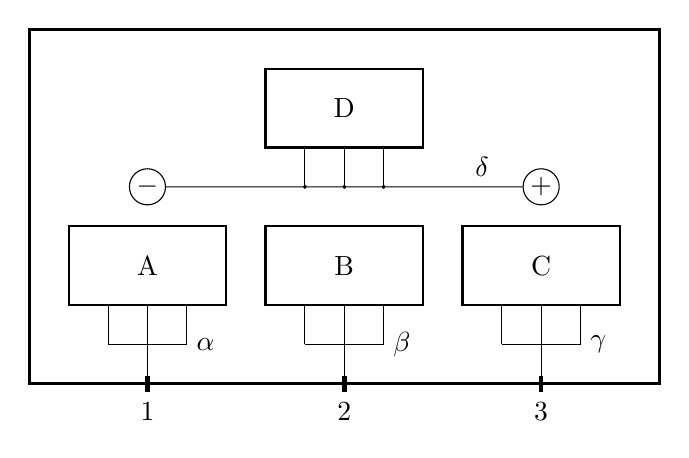
\begin{tikzpicture}[scale=0.5]
  \draw[very thick] (0, 0) rectangle +(16, 9);
%  \draw (-0.1, 1.5) -- (2, 1.5) node[right] {\tt (};
%  \draw (4, 1.5) node[left] {\tt )} -- (6.1, 1.5);

  \draw[thick] (1, 2) rectangle node {A} +(4, 2);
  \draw[thick] (6, 2) rectangle node {B} +(4, 2);
  \draw[thick] (11, 2) rectangle node {C} +(4, 2);
  \draw[thick] (6, 6) rectangle node {D} +(4, 2);

  \node[draw,circle,inner sep=1pt] at (3, 5) (minus) {$-$};
  \node[draw,circle,inner sep=1pt] at (13, 5) (plus) {$+$};

  \node at (11.5, 5.5) {$\delta$};
  
  % connexion minus / plus et veers D.
  \draw (minus) -- (7, 5) circle[fill=black,radius=1pt] -- (8, 5) circle[fill=black,radius=1pt] -- (9, 5) circle[fill=black,radius=1pt] -- (plus);
  \draw (7, 5) -- (7, 6);
  \draw (8, 5) -- (8, 6);
  \draw (9, 5) -- (9, 6);

  \begin{scope}
    \draw[ultra thick] (3, -0.2) -- +(0, 0.4) node[below=2mm] {1};
    \draw (3, 0) -- (3, 1);
    \draw (2, 1) -- (4, 1) node[right] {$\alpha$};
    \draw (2, 1) -- (2, 2);
    \draw (3, 1) -- (3, 2);
    \draw (4, 1) -- (4, 2);
  \end{scope}
  \begin{scope}[xshift=5cm]
    \draw[ultra thick] (3, -0.2) -- +(0, 0.4) node[below=2mm] {2};
    \draw (3, 0) -- (3, 1);
    \draw (2, 1) -- (4, 1) node[right] {$\beta$};
    \draw (2, 1) -- (2, 2);
    \draw (3, 1) -- (3, 2);
    \draw (4, 1) -- (4, 2);
  \end{scope}
  \begin{scope}[xshift=10cm]
    \draw[ultra thick] (3, -0.2) -- +(0, 0.4) node[below=2mm] {3};
    \draw (3, 0) -- (3, 1);
    \draw (2, 1) -- (4, 1) node[right] {$\gamma$};
    \draw (2, 1) -- (2, 2);
    \draw (3, 1) -- (3, 2);
    \draw (4, 1) -- (4, 2);
  \end{scope}  
\end{tikzpicture}
\end{center}
\caption{\label{fig:quadraticE} \sout{botched attempt at 3-Dyck} Maze showing that the number of edges in the dual representation graph can be quadratic in the number of wires.}
\end{figure}

However, the dual representation of the maze can have $E = \bigOmega{W^2}$
edges. This is for instance the case of the maze show in
Fig.~\ref{fig:quadraticE}: there are $k+1$ wires, and except the special one
that it connected to $\oplus$ and $\ominus$, they are all reachable from one
another. So the dual representation graph has $k(k+1)$ edges.

It follows that the generic technique may require $\bigOmega{B W^4}$
operations. However, the context-free grammar, once constructed, reveals much
information about the language. In particular, it is fairly easy to find the
shortest path that exits the maze (associate to each non-terminal the shortest
word that can be obtained from it, and take the minimum over each possible
derivation rule).

\section{Getting out of recursive mazes faster with inter-dimensional wormholes}
\label{sec:modelchecking}


There is a more efficient technique that can be better suited to laaaaaarge
recursive mazes. It is heavily inspired by algorithms designed almost
simultaneously by Bouajjani, Esparza and
Maler~\cite{DBLP:conf/concur/BouajjaniEM97} on the one hand and Finkel, Willems
and Wolper~\cite{DBLP:journals/entcs/FinkelWW97} on the other hand. These
algorithms were created to decide reachability properties in pushdown systems,
in the context of model checking problems that could admit such a
representation.

The main idea behind this algorithm is simple. If there are two edges
$\alpha \xrightarrow{X.i} \beta \xleftarrow{X.j} \gamma$ in the dual
representation graph, then it is possible to move from $\alpha$ to $\gamma$ as
follows: starting from wire $\alpha$, enter the recursive box $X$ using its
$i$-th pin (this lands on wire $\beta$ inside $X$), then leave $X$ using its
$j$-th pin (this lands on wire $\gamma$ outside of $X$). Of course, the return trip is also possible.

More generally, if there is a sequence of instructions $S$ that allows the
player to travel from wire $\beta$ to wire $\gamma$ while exiting box $X$
(popping $X$ from the stack), then $X.i ; S$ is a sequence of instructions that
allows the player to travel from $\alpha$ to $\gamma$ while leaving the stack
unchanged. This is the main idea underlying the construction of the context-free
grammar given above.

We therefore define a binary relation $\equiv$ between wires, where
$\alpha \equiv \gamma$ if and only if there is a box $X$ and two pins $i, j$
such that the two edges $\alpha \xrightarrow{X.i} \beta \xleftarrow{X.j} \gamma$
exist in the dual representation graph. In this case we say that there is a
\emph{local wormhole} between $\alpha$ and~$\gamma$. Note that $\equiv$ is
symmetric, but not necessarily reflexive nor transitive. We then consider the
following sequence of pairs of wires:
\begin{align*}
  \Gamma_0 &= \{ (\alpha, \beta) ~|~ \alpha \equiv \beta \} \cup \{ (\omega, \omega) ~|~ \omega \in \mathcal{W} \} \\
  \Gamma_{i+1} &= \Gamma_i \cup \{ (\alpha, \gamma) ~|~ \exists \beta. ~ (\alpha, \beta) \in \Gamma_i, (\beta, \gamma) \in \Gamma_i \} \\
           & ~\quad \phantom{\Gamma_i} \cup \{ (\alpha, \delta) ~|~ \exists \beta. ~ \exists \gamma. ~ (\alpha, \beta) \in \Gamma_i, \beta \equiv \gamma, (\gamma, \delta) \in \Gamma_i \}
\end{align*}
The sequence $\Gamma_i$ is increasing (with respect to set inclusion) and
upper-bounded by $\mathcal{W} \times \mathcal{W}$, therefore it converges (in a
finite number of steps) to a limit denoted as $\Gamma_\infty$. We write
$\alpha \equiv_i \beta$ (resp. $\alpha \stackrel{*}{\equiv} \beta$) as
syntactic sugar for $(\alpha, \beta) \in \Gamma_i$ (resp. $\Gamma_\infty$).

\medskip

\begin{lemma}
  $\stackrel{*}{\equiv}$ is the smallest equivalence relation such that
  $\alpha \xrightarrow{X.i} \beta \stackrel{*}{\equiv} \gamma \xleftarrow{X.j}
  \delta \Longrightarrow \alpha \stackrel{*}{\equiv} \delta$.
\end{lemma}
\begin{proof}
  By intimidation: if this is not obvious to the reader, then they better stop
  reading \emph{RIGHT NOW}! (otherwise, the argument is that the $\Gamma_i$ are
  constructed to this purpose; $\stackrel{*}{\equiv}$ is the least fixed-point
  of the increasing function on pairs of wires that guarantees the wanted properties).
\end{proof}

The idea is that there is a sequence of instruction that takes the player from
$\alpha$ to $\delta$ while leaving the stack unchanged whenever
$\alpha \stackrel{*}{\equiv} \delta$. We then say that there is a
\emph{transitive wormhole} between $\alpha$ and $\delta$.

Most games that require the player to explore a large map have some built-in
mechanism to ``fast-travel'' between some previously visited
locations. Recursive mazes lack this mechanism, and that is really
unfortunate. For this reason, we suggest to extend the game with the ability to
fast-travel through wormholes (and we bet that this could relieve players of a
considerable amount of frustration). We extend the usual semantic of the
dual representation graph with these wormholes, using dashed edges:

\begin{center}
  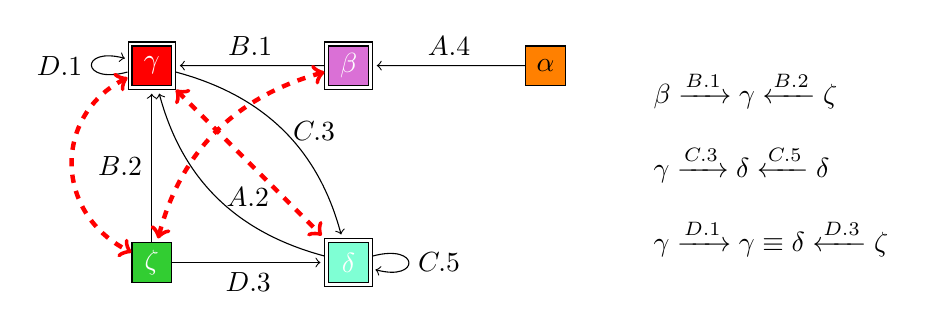
\begin{tikzpicture}[scale=1.25]
    \node[wire,fill=orange] at (4, 2) (start) {$\alpha$};
    \node[wire,fill=LimeGreen,text=white] at (0, 0) (G) {$\zeta$};
    
    \node[wire,fill=red,text=white] at (0, 2) {$\gamma$};
    \node[draw,minimum size=6mm] at (0, 2) (R) {};
    \node[wire,fill=Aquamarine,text=white] at (2, 0) {$\delta$};
    \node[draw,minimum size=6mm] at (2, 0) (B) {};
    \node[wire,fill=Orchid,text=white] at (2, 2) {$\beta$};
    \node[draw,minimum size=6mm] at (2, 2) (K) {};
    
    \draw (start) edge[->] node[above] {$A.4$} (K);

    \draw (K) edge[->] node[above] {$B.1$} (R);

    \draw (B) edge[->, "$C.5$", loop right] (C);
    \draw (B) edge[->, bend left] node[right] {$A.2$} (R);
    \draw (G) edge[->] node[below] {$D.3$} (B);

    \draw (R) edge[->, "$D.1$", loop left] (R);
    \draw (G) edge[->] node[left] {$B.2$} (R);
    \draw (R) edge[->, bend left] node[right] {$C.3$} (B);

    \draw (K) edge[<->, red, ultra thick, dashed, bend right] (G);
    \draw (R) edge[<->, red, ultra thick, dashed] (B);
    \draw[<->, red, ultra thick, dashed] (R) .. controls (-1, 1.5) and (-1, 0.5) .. (G);

    \node[anchor=west] at (5, 1.75) {$\beta \xrightarrow{B.1} \gamma \xleftarrow{B.2} \zeta$};
    \node[anchor=west] at (5, 1) {$\gamma \xrightarrow{C.3} \delta \xleftarrow{C.5} \delta$};
    \node[anchor=west] at (5, 0.25) {$\gamma \xrightarrow{D.1} \gamma \equiv \delta \xleftarrow{D.3} \zeta$};
  \end{tikzpicture}
\end{center}

Note that the wormhole between $\gamma$ and $\zeta$ is transitive
($\gamma \not\equiv \zeta$ but $\gamma \stackrel{*}{\equiv} \zeta$). From this,
we observe that
$\alpha \xrightarrow{A.4} \beta \stackrel{*}{\equiv} \gamma \xleftarrow{A.2}
\delta$, so that $\alpha \stackrel{*}{\equiv} \delta$ and the maze can be
exited from the starting wire.

The algorithm described in
\cite{DBLP:conf/concur/BouajjaniEM97,DBLP:journals/entcs/FinkelWW97} essentially
consists in explicitly computing $\stackrel{*}{\equiv}$ by iterating the
recursive construction starting from $\equiv$ until a least fixed point has been
reached. This algorithm has complexity cubic in the number of states of the
automaton. In our context, this leads to an algorithm with complexity
$\bigO{W^3}$, which is already better than constructing the associated
context-free grammar.

This algorithm adds all the possible wormhole edges to the dual representation
graph (at most $W^2$ of them). Each edge can be labelled with a unique
identifier. Local wormhole edges can additionally be labelled with a sequence of
\emph{two} instructions. Transitive wormhole edges can be labelled with a tuple
of (instruction, wormhole identifier, instruction). All wormhole edges can be
labelled with a length. Therefore, not only it is possible to find a the
shortest path from the starting point to an exit (using only wormhole edges),
but it is possible to emit a description of this path in polynomial time, even
though the path may have exponential length, by printing the labels of the
crossed wormhole edges.

In passing, \cite{DBLP:conf/concur/BouajjaniEM97,DBLP:journals/entcs/FinkelWW97}
show that the set of stacks that the player can have when sitting on a given
wire is a regular language (accepted by a deterministic finite automaton).

\section{Getting out of recursive mazes even faster by collapsing wormholes}
\label{sec:us}


The main contribution of this paper is that, in the case of recursive mazes, it
is possible to do better
than~\cite{DBLP:conf/concur/BouajjaniEM97,DBLP:journals/entcs/FinkelWW97}. Our
starting point is that the reversible nature of all movements makes it possible
to exploit equivalence classes of wires. If $\alpha \stackrel{*}{\equiv} \beta$,
then we are going to consider that $\alpha$ and $\beta$ are ``the same wire'',
and as far as reachability is concerned no information is lost by doing so.

This is different from the general problem tackled
by~\cite{DBLP:conf/concur/BouajjaniEM97,DBLP:journals/entcs/FinkelWW97} of
deciding reachability of a given state in an arbitrary pushdown automaton. The
main difference is that in a general PDA there may be a sequence of transitions
from a state $q$ to another state $q'$ that leaves the stack unchanged, while
there might not be a sequence of transitions from $q'$ to $q$ that leaves the
stack unchanged. In recursive mazes, we now that the latter exists.

This makes it possible for us, instead of explicitly building a clique between
equivalent wires as
in~\cite{DBLP:conf/concur/BouajjaniEM97,DBLP:journals/entcs/FinkelWW97}, to
build a (much smaller) \emph{spanning tree}: this preserves reachability
properties. The same technique is used in the context of sparse matrix
factorization~\cite{osti_834431} to construct the elimination tree of the matrix
$A^t A$, given a sparse matrix $A$ and without explicitly forming $A^t A$ that
might be much denser. Each row of $A$ with $k$ non-zero entries creates a clique
of size $k$ in the graph whose adjacency matrix is $A^t A$. This clique is
replaced by a path that preserves reachability.

Our proposed solution is also inspired by the ``edge-contracting'' probabilistic
algorithm of Karger for min-cut~\cite{DBLP:conf/soda/Karger93}. The core idea of
our proposal is simple: when a local wormhole
$\alpha \xrightarrow{X.i} \beta \xleftarrow {X.j} \gamma$ is identified, we add
an edge \raisebox{-4.5pt}{\tikz{\node (x) {$\alpha$}; \node at (1.3, 0) (y)
    {$\gamma$}; \draw[red,dashed,ultra thick,<->] (x) -- (y);}} to the
dual representation graph, and we immediately contract it. This collapses the
two nodes that are the extremities of the wormhole into one and deletes the
newly added edge. The reader may wonder what was the point of adding add edge
just before deleting it. So, OK, let's not add it, and instead directly
``merge'' the two equivalent wires. This operation creates a \emph{supernode}
labelled with a set of wires ($\{\alpha, \gamma\}$ if starting from $\alpha$ and
$\gamma$), as opposed to a normal node labelled with a single wire. All edges
originating from (resp. pointing towards) the original nodes now originate in
(resp. point to) the new supernode. The two edges forming the local wormhole now
have the same extremities and the same box attribute, so we remove one of
them. See Fig.~\ref{fig:merge} for an illustration. The underlying idea is that
all wires inside of a supernode are known to be in relation by
$\stackrel{*}{\equiv}$. Our algorithm consists in iterating this graph rewriting
process as long as possible\footnote{After a draft of this paper was written, we
  discovered that the same operation has been called ``folding''
  in~\cite{Stallings1983,b97de931-5994-30c4-b01e-c43e12a3f8e6,STEINBERG2002341},
  in quite a different context---profinite topologies on a free group}.


\tikzset{every edge/.style={draw,shorten >=0.5mm}}

\begin{figure}
\centering
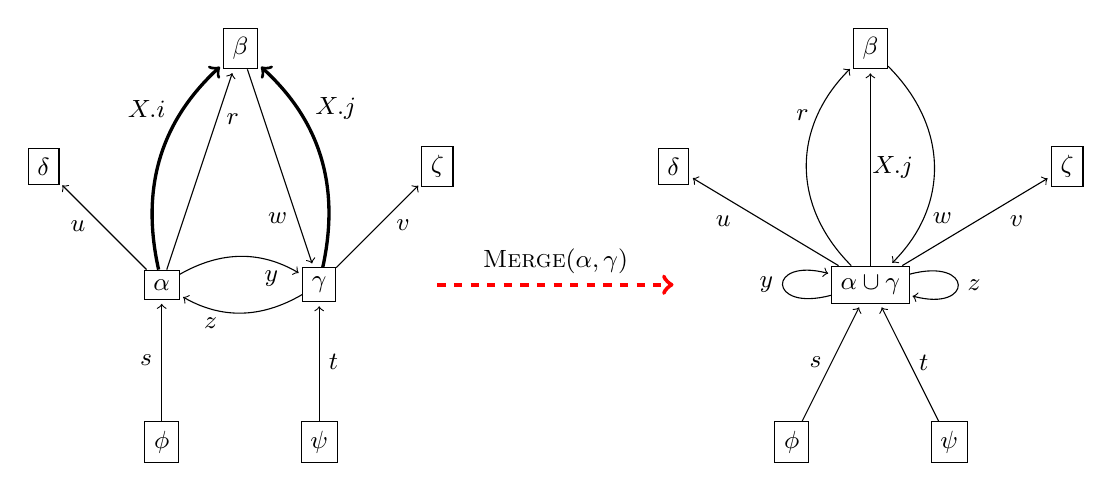
\begin{tikzpicture}[every node/.style={font=\small}, every edge/.style={draw,shorten >=0.5mm}]
  \begin{scope}
  \node[draw] at (0, 0) (a) {$\alpha$};
  \node[draw] at (2, 0) (c) {$\gamma$};
  \node[draw] at (1, 3) (b) {$\beta$};
  \node[draw] at (-1.5, 1.5) (d) {$\delta$};
  \node[draw] at (3.5, 1.5) (e) {$\zeta$};
  \node[draw] at (0, -2) (f) {$\phi$};
  \node[draw] at (2, -2) (g) {$\psi$};

  \draw (a) edge[->,very thick, bend left] node[left=1mm, near end] {$X.i$} (b);
  \draw (c) edge[->,very thick, bend right] node[right=1mm, near end] {$X.j$} (b);
  
  \draw (a) edge[->,bend left] node[below, near end] {$y$} (c);
  \draw (c) edge[->,bend left] node[below, near end] {$z$} (a);

  \draw (a) edge[->] node[right, near end] {$r$} (b);
  \draw (a) edge[->] node[left=1mm] {$u$} (d);
  
  \draw (b) edge[->] node[left, near end] {$w$} (c);
  \draw (c) edge[->] node[right=1mm] {$v$} (e);
  \draw (f) edge[->] node[left] {$s$} (a);
  \draw (g) edge[->] node[right] {$t$} (c);
\end{scope}

\draw[ultra thick, red, dashed, ->] (3.5, 0) -- node[black,above] {\textsc{Merge}$(\alpha, \gamma)$} (6.5, 0);

\begin{scope}[xshift=8cm]
  \node[draw] at (1, 0) (ac) {$\alpha \cup \gamma$};
  \node[draw] at (1, 3) (b) {$\beta$};
  \node[draw] at (-1.5, 1.5) (d) {$\delta$};
  \node[draw] at (3.5, 1.5) (e) {$\zeta$};
  \node[draw] at (0, -2) (f) {$\phi$};
  \node[draw] at (2, -2) (g) {$\psi$};

  \draw (ac) edge[->,loop left] node[left] {$y$} (ac);
  \draw (ac) edge[->,loop right] node[right] {$z$} (ac);
  \draw (ac) edge[->] node[right=-1mm] {$X.j$} (b);

  \draw[->,shorten >=0.5mm] (ac) .. controls (0, 1) and (0, 2) .. node[left=0mm, near end] {$r$}  (b);
  \draw[->,shorten >=0.5mm] (b)  .. controls (2, 2) and (2, 1) .. node[right=0mm, near end] {$w$} (ac);

  \draw (ac) edge[->] node[left=3mm] {$u$} (d);
  \draw (ac) edge[->] node[right=3mm] {$v$} (e);
  \draw (f) edge[->] node[left] {$s$} (ac);
  \draw (g) edge[->] node[right] {$t$} (ac);
\end{scope}
\end{tikzpicture}
\caption{\label{fig:merge} Illustration of the graph contraction process. Edge labels in lower-case letters are arbitrary.}
\end{figure}

%\subsection{Correctness}

We now establish the main property of the process: wormholes can be contracted
in any order, and at the end we get exactly the equivalence classes of
$\stackrel{*}{\equiv}$.

The intuition behind this is that contracting a wormhole may create new
wormholes but not destroy preexisting ones (other than the one being contracted,
of course). This is because a wormhole requires two similarly-labelled edges
pointing to the same node ; contracting a wormhole can only bring together the
endpoints of edges previously pointing to different nodes, not take them apart.

We formally establish the results using tools borrowed from the field of
\sout{artificial intelligence} automated reasoning (and more precisely,
rewriting techniques for equational theories,
see~\cite{DBLP:books/el/RV01/DershowitzP01} for more details).  Let $\leadsto$
be the binary relation on directed graphs that corresponds to the wormhole
contraction process described above. It operates on graphs where edges are
labelled by a (box, pin) pair, and where nodes are labelled with a set of
wires. We have $G \leadsto G'$ if $G'$ can be obtained from $G$ by contracting a
wormhole. In this case, $G'$ has one less vertex and one less edge than $G$. It
follows that any \emph{derivation} $G_0 \leadsto G_1 \leadsto \dots$ is
finite. Let $\stackrel{*}{\leadsto}$ denote the reflexive-transitive closure of
$\leadsto$. A graph $G$ is \emph{reducible} if there is a $G'$ such that
$G \leadsto G'$, and \emph{irreducible} otherwise. When
$G \stackrel{*}{\leadsto} G'$ and $G'$ is irreducible, then $G'$ is a
\emph{normal form} of $G$. In our case, normal forms are \emph{unique}: if $G_0$
and $G_1$ are normal forms of $G$, then $G_0 = G_1$.  The main ingredient to
establish this is the following:

\medskip

\begin{lemma}
  The $\leadsto$ relation is \emph{confluent}: if $G \stackrel{*}{\leadsto} G_0$ and
  $G \stackrel{*}{\leadsto} G_1$, then there is a $G'$ such that
  $G_0 \stackrel{*}{\leadsto} G'$ and $G_1 \stackrel{*}{\leadsto} G'$.
\end{lemma}

\begin{proof}
  This follows from \emph{strong confluence} and termination of $\leadsto$ by
  Newman's lemma (essentially, an induction on the number of steps of the
  derivations).

  Therefore the problem is to prove strong confluence: if $G \leadsto G_0$ and
  $G \leadsto G_1$, then either $G_0 = G_1$ or there is a $G'$ such that
  $G_0 \leadsto G'$ and $G_1 \leadsto G'$. Suppose $G_0 \neq G_1$, so that there
  are two ``contractible'' wormholes in $G$:
  $\alpha \xrightarrow{X} \beta \xleftarrow{X} \gamma$ (leading to $G_0$) and
  $\phi \xrightarrow{Y} \chi \xleftarrow{Y} \psi$ (leading to $G_1$), with
  $\{ \alpha, \gamma \} \neq \{\phi, \psi\}$.

  If $\{ \alpha, \gamma \} \cap \{\phi, \psi\} = \emptyset$, then after
  contracting $\alpha \xrightarrow{X} \beta \xleftarrow \gamma$ (yielding
  $G_0$), there still exist two vertices labelled $\phi$ and $\psi$ in $G_0$,
  along with the two outgoing edges labelled $Y$ pointing to the same node
  $\chi'$ (even though $\chi'$ may not be labelled $\chi$ as in $G$ as a result
  of the contraction; in any case it is labelled with a superset of
  $\chi$). Contracting $\phi \xrightarrow{Y} \chi' \xleftarrow{Y} \psi$ is still
  possible in $G_0$ and yields $G'$, where $\alpha, \gamma, \phi$ and $\psi$
  have been replaced by $\alpha \cup \gamma$ and $\psi \cup \phi$. The exact
  same reasoning can be carried out starting from $G_1$ (contracting the other
  wormhole), with the same conclusion.

  if $\{ \alpha, \gamma \} \cap \{\phi, \psi\} \neq \emptyset$, then without
  loss of generality we may assume that $\phi = \gamma$. There are thus two
  wormholes
  $\alpha \xrightarrow{X} \beta \xleftarrow{X} \gamma \xrightarrow{Y} \chi
  \xleftarrow{Y} \psi$. In that case, after contracting
  $\alpha \xrightarrow{X} \beta \xleftarrow \gamma$, we see that the second
  wormhole has been modified: $\gamma \xrightarrow{Y} \chi \xleftarrow{Y} \psi$
  in $G$ has been replaced by
  $(\alpha \cup \gamma) \xrightarrow{Y} \chi' \xleftarrow{Y} \psi$ in $G_0$. But
  then, contracting the modified wormhole leads to $G'$, where $\alpha, \gamma$
  and $\psi$ have been replaced by a single vertex
  $\alpha \cup \gamma \cup \psi$. Again, the same reasoning can be made starting
  from the other wormhole, yielding the same graph.
\end{proof}

\begin{corollary}
  Normal forms for $\leadsto$ are unique (and are obtained after a finite number
  of steps).
\end{corollary}

So, the non-determinism that appears when several wormholes coexist is not
important. Wormholes can be contracted in any order, and we always obtain the
same result---a good one.

\medskip

\begin{theorem}\label{thm:correctness}
  Let $G$ be the dual representation graph of a recursive maze, and $G_{nf}$ a
  normal form of $G$ for $\stackrel{*}{\leadsto}$. Then the nodes of $G_{nf}$
  are labelled by the equivalence classes of $\stackrel{*}{\equiv}$.
\end{theorem}

This theorem follows from the two following lemmas, using the same notations as
the theorem.

\medskip

\begin{lemma}
  Wires in a supernode of $G_{nf} $are related by $\stackrel{*}{\equiv}$.
\end{lemma}

\begin{proof}
  Consider a derivation
  $G = G_0 \leadsto G_1 \leadsto \dots \leadsto G_k = G_{nf}$ leading to the
  normal form. The result is established by induction on $i$. When $i=0$, nodes of
  $G$ are labelled by singletons, so the property trivially holds.

  Next, suppose the property holds in $G_i$. The next graph $G_{i+1}$ is
  obtained by contracting a wormhole
  $\Sigma \xrightarrow{X} \Theta \xleftarrow{X} \Pi$, thus ``merging'' $\Sigma$
  and $\Pi$. The two edges forming the wormhole existed in the original graph
  $G$: in $G$ there are $\alpha \xrightarrow{X} \beta$ and
  $\gamma \xrightarrow{X} \delta$, where $\alpha \in \Sigma$,
  $\beta, \gamma \in \Theta$ and $\delta \in \Pi$. By induction hypothesis,
  $\beta \stackrel{*}{\equiv} \gamma$ (they both belong to the supernode
  $\Theta$). This means that $\alpha \stackrel{*}{\equiv} \delta$ (by definition
  of $\stackrel{*}{\equiv}$). Now the fact that any pair
  $(\sigma, \pi) \in \Sigma \times \Pi$ are related by $\stackrel{*}{\equiv}$
  follows from the transitivity of $\stackrel{*}{\equiv}$ and from the induction
  hypothesis applied to $\Sigma$ and $\Pi$.
\end{proof}

\begin{lemma}
  For any $i \geq 0$, if $\alpha \equiv_i \beta$, then $\alpha$ and $\beta$
  belong to the same supernode in $G_{nf}$.
\end{lemma}

\begin{proof}
  We prove the result by induction on $i$.  When $i=0$, we need to show that
  wires that are connected by a local wormhole in $G$ have been contracted in
  $G_{nf}$. Starting from $G$, we first contract an arbitrary wormhole
  $\alpha \xrightarrow{X} \beta \xleftarrow{X} \gamma$, leading to $G_1$
  ($G \leadsto G_1$). Then by the confluence of $\leadsto$, we know that
  $G_1 \stackrel{*}{\leadsto} G'$. In other term, $\alpha$ and $\gamma$ belong
  to the same supernode in $G_{nf}$. This is true for any wormhole initially
  present in $G$.

  Next, suppose the result holds for $i \geq 0$, and take two wires
  $\alpha \equiv_{i+1} \beta$. Looking at the definition of $\Gamma_{i+1}$,
  there are 3 cases to consider:
\begin{itemize}
\item $\alpha \equiv_{i} \beta$. In this case, the result directly holds by induction hypothesis.
\item There is a wire $\gamma$ such that $\alpha \equiv_{i} \gamma$ and
  $\gamma \equiv_{i} \beta$. By induction hypothesis, $\alpha, \beta$ and
  $\gamma$ all belong to the same supernode.
\item There are two wires $\gamma$ and $\delta$ and a box $X$ such that
  $\alpha \xrightarrow{X} \gamma$, $\gamma \equiv_i \delta$ and
  $\delta \xleftarrow{X} \beta$. By induction hypothesis, $\gamma$ and $\delta$
  belong to the same supernode (say $\Theta$) in $G_{nf}$. Suppose, for the sake
  of a contradiction that, in $G_{nf}$, $\alpha$ belongs to a supernode $\Sigma$
  and that $\beta$ belongs to a different supernode $\Pi$. Then the two edges
  $\alpha \xrightarrow{X} \gamma$ and $\beta \xrightarrow{X} \delta$ of $G$ have
  not been removed in $G_{nf}$, but were modified to become
  $\Sigma \xrightarrow{X} \Theta \xleftarrow{X} \Pi$. Therefore, there is a
  contractible wormhole in $G_{nf}$, which contradicts the irreducibly of
  $G_{nf}$.
\end{itemize}
\end{proof}

We now discuss the implications of theorem~\ref{thm:correctness}. Starting from
the dual representation graph of a maze, run the contraction process until a
normal form has been obtained. To check if it is possible to exit the maze, it
is sufficient to examine the wires in the equivalence class of the starting
point, and test if one of them is connected to an outer IO pin. When it is the
case, an exit path can be built explicitly (but how to do so depends on
implementation details discussed below).

\section{Efficient deterministic implementations}
\label{sec:implem}

We now discuss the efficient implementation of the graph rewriting process
discussed above. We assume that everything is represented as word-sized
integers: wires are numbered from 0 to $W-1$, boxes are numbered from 0 to
$B-1$, etc. The input is the dual representation graph, provided as adjacency
lists, i.e. as an array \texttt{G} such that $\texttt{G}[\omega]$ is the
(linked) list of edges coming out of node $\omega$. The edge
$\alpha \xrightarrow{X.i} \beta$ is represented by the triplet $(X, i, \beta)$,
where the endpoint is explicit and the starting point is implicit. We therefore
define the ``type''
$\texttt{edge} ::= \texttt{box} \times \texttt{pin} \times \texttt{wire}$ (these
are actually 3 integers, but this spells out their purpose more explicitly). The
graph is therefore provided as an \texttt{edge list array}, where the edges
coming out of wire $\omega$ are given in $\texttt{G}[\omega]$.

Tuples, also known as records or \texttt{struct}, can be (de)constructed in
constant time. We make abundant use of \sout{blockchains} linked lists, and we
employ the following notations:
\begin{itemize}
\item \texttt{[]} denotes the empty list (a \texttt{NULL} pointer).
\item $L \gets \texttt{head} :: \texttt{tail}$ denotes the operation that constructs a
  new linked $L$ list whose first element is \texttt{head}, followed by the linked
  list \texttt{tail} (this means that a new cell must be acquired, \texttt{head}
  must be copied into it, and a pointer to \texttt{tail} must also be stored).
\item $\texttt{head} :: \texttt{tail} \gets L$ denotes the ``deconstruction''
  operation: it fetches the data item \texttt{head} contained in the first entry
  of the list, and grabs a pointer \texttt{tail} to the remaining items.
\end{itemize}
(De)constructing a list runs in constant time, and so does accessing any
location in an array. The observant reader may have noticed that our notations
are inspired from functional languages from the ML family.

We keep a list (\texttt{pending}) of wormholes awaiting contraction, and process
them one at a time, adding newly discovered wormholes to the list. We must
however navigate around two problems:
\begin{enumerate}
\item The same pair of wires can be merged by two (or more) wormholes (as shown
  in Fig.~\ref{fig:wormholes-pb}, left). In our implementation, the pending list
  may contain several wormholes merging the same pair of nodes.

\item The number of wormholes can be quadratic in the size of the maze, even if
  it has only $E = \bigO{W}$ edges (see Fig.~\ref{fig:wormholes-pb},
  right). However, not all of them can be collapsed: some will vanish into thin
  air when \emph{others} are collapsed.
\end{enumerate}

When processing the next wormhole, we check if the two wires have already been
merged and only proceed when it is not the case (this solves the first problem).

When a wormhole $\alpha \xrightarrow{X.i} \beta \xleftarrow {X.j} \gamma$ is
discovered and added to the list, we immediately remove one of the two edges
from the graph---they would become identical later when the wormhole actually
gets contracted and one of them would be removed anyway, so why delay the
inevitable?  With this modification, only $E$ wormholes can be added to the
list. We implement this as follows: we look at each edge of the initial graph in
sequence: either it creates a wormhole with another ``hot'' edge (we register
the wormhole and original the edge is sucked into the void), or it does not (we
mark the edge as hot).

\begin{figure}
  \centering
  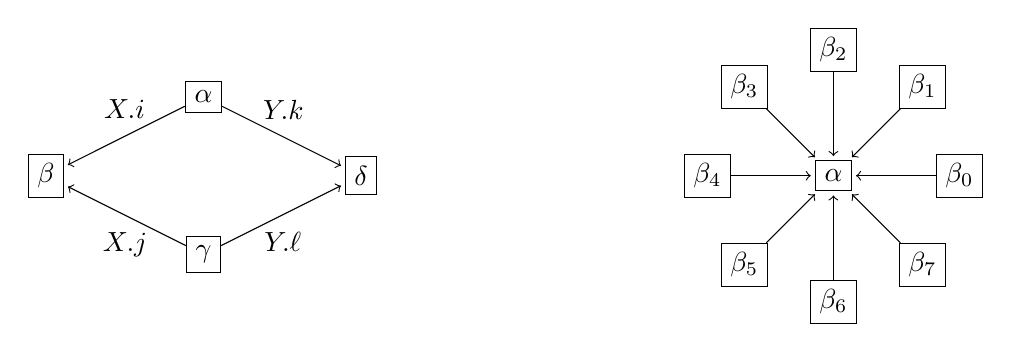
\begin{tikzpicture}
  \node[draw ]at (0, 0) (b) {$\beta$};
  \node[draw] at (2, 1) (a) {$\alpha$};
  \node[draw] at (2, -1) (c) {$\gamma$};
  \node[draw] at (4, 0) (d) {$\delta$};

  \draw (a) edge[->] node[above=1mm] {$X.i$} (b);
  \draw (c) edge[->] node[below=1mm] {$X.j$} (b);

  \draw (a) edge[->] node[above=1mm] {$Y.k$} (d);
  \draw (c) edge[->] node[below=1mm] {$Y.\ell$} (d);

  \begin{scope}[xshift=10cm]
    \node[draw] at (0, 0) (a) {$\alpha$};

    \foreach \d in {0, 1, ..., 7}
      \node[draw] at (45*\d:1.6cm) (b) {$\beta_\d$} edge[->] (a);
  \end{scope}
\end{tikzpicture}
\caption{\label{fig:wormholes-pb}Two wires can be merged by several wormholes (left). There can be a
  quadratic number of wormholes (right).}
\end{figure}

Inside each supernode, one node is chosen as ``supernode leader''. The supernode
is hosted by the leader node in the original graph. Nodes that have been merged
into larger supernode are not actually removed from the graph ; they remain
there but become \emph{followers} (as opposed to their leader).

When two (super)nodes are merged, to form the resulting supernode, one of them
is ``absorbed'' into the other one. Hot edges pointing to the absorbee either
create a wormhole and are dropped, or become hot edges pointing to the absorber.
The actual issue is to detect the new wormholes that are created by the
displacement of edges.

A major difference with the process suggested by Fig.~\ref{fig:merge} is that we
only move the targets of edges, not their origins. This does not affect the
process, at least not until an actual exit path has to be constructed. This
issue is discussed in section~\ref{sec:arg}.

\subsection{Dense mazes}
\label{sec:dense}

We first describe a simple implementation tailored for the case of \emph{dense}
mazes, where $E \approx WB$. We use a \texttt{hot} array of dimension
$W \times B$ such that $\texttt{hot}[\beta,X]$ is either \texttt{none} or
$\texttt{some} (\alpha, i)$, in which case there is a ``hot'' edge
$\alpha \xrightarrow{X.i} \beta$ in the graph. % Initializing the \texttt{hot}
% array takes time $\bigO{BW}$.

When the algorithm starts, each node in the graph corresponds to a wire of the
maze. Then nodes will be merged into supernodes. Maintaining the content of
supernodes is a once-in-a-lifetime chance for us to use the celebrated
``inverse-Ackermann'' disjoint-set data structure (also known as
\textsc{Union-Find}). This uses the two arrays \texttt{parent} and \texttt{rank}.

The pseudo-code of our solution in shown as Algorithm~\ref{algo:main-dense}. We
believe that it is simple enough to be implemented in assembler by a motivated
undergraduate student. Its step-by-step execution on the simple maze of
Fig.~\ref{fig:simple} is shown in Fig.~\ref{fig:step-by-step}. When it
terminates, equivalence classes of $\stackrel{*}{\equiv}$ have been
determined. This easily allows to test if the maze can be exited.

\begin{algorithm}
\begin{algorithmic}[1]
  \Function{Find}{$\alpha$}
  \If{$\texttt{parent}[\alpha] \neq \alpha$}           \Comment{path compression}
  \State $\texttt{parent}[\alpha] \gets \Call{Find}{\texttt{parent}[\alpha]}$
  \EndIf
  \State \Return $\texttt{parent}[\alpha]$
  \EndFunction

  \bigskip
  
  % an edge either becomes hot or creates a wormhole
  \Procedure{AddEdge}{$\alpha, X, i, \beta$}
   \If{$\texttt{hot}[\beta, X] = \texttt{some} (\gamma, j)$}
   \State $\texttt{pending} \gets (\alpha, X, i, \beta, j, \gamma)) :: \texttt{pending}$       \Comment{detected $\alpha \xrightarrow{X.i} \beta \xleftarrow{X.j} \gamma$}
   \Else
   \State $\texttt{hot}[\beta, X] \gets \texttt{some} (\alpha, i)$   
   \EndIf
   \EndProcedure

  \bigskip

  \Procedure{Merge}{$\sigma, \pi$}                                    
  \If{$\texttt{rank}[\pi] < \texttt{rank}[\sigma]$}                               \Comment{\textsc{Union}}
  \State $\texttt{tmp} \gets \pi, \pi \gets \sigma, \sigma \gets \texttt{tmp}$    \Comment{Union-by-rank: $\sigma$ is absorbed in $\pi$}
  \EndIf
  \State $\texttt{parent}[\sigma] = \pi$
  \If{$\texttt{rank}[\sigma] = \texttt{rank}[\pi]$}
  \State increment $\texttt{rank}[\pi]$
  \EndIf
  \For{$0 \leq X < B$}                                                    \Comment{Transfer hot edges}
    \If{$\texttt{hot}[\sigma, X] \neq \texttt{none}$}
      \State $\texttt{some} (\omega, i) \gets \texttt{hot}[\sigma, X]$    \Comment{looking at $\omega \xrightarrow{X.i} \sigma$}
      \State $\Call{AddEdge}{\omega, X, i, \pi}$                          \Comment{replace by $\omega \xrightarrow{X.i} \pi$}
    \EndIf
  \EndFor  
  \EndProcedure

  \bigskip

  \Procedure{CollapseMazeDense}{$W, B, \texttt{G}$}                          
  \State $\texttt{pending} \gets \texttt{[]}$                           \Comment{Setup}
  \For{$0 \leq \alpha < W$}
    \State $\texttt{parent}[\alpha] \gets \alpha$                       \Comment{$\alpha$ is a supernode by itself}
    \State $\texttt{rank}[\alpha] \gets 0$
    \For{$0 \leq X < B$}
    \State $\texttt{hot}[\alpha,X] \gets \texttt{none}$                 
    \EndFor
    \For{each $(X, i, \beta)$ in $\texttt{G}[\alpha]$}                  \Comment{prime the wormhole pump} 
      \State $\Call{AddEdge}{\alpha, X, i, \beta}$
    \EndFor
  \EndFor

  \While{$\texttt{pending} \neq \texttt{[]}$}                                   \Comment{main loop : process known wormholes}
  \State $(\alpha, X, i, \beta, j, \gamma) :: \texttt{tail} \gets \texttt{pending}$     \Comment{popped $\alpha \xrightarrow{X.i} \beta \xleftarrow{X.j} \gamma$}
  \State $\texttt{pending} \gets \texttt{tail}$    
  \State $\sigma \gets \Call{Find}{\alpha}$
  \State $\pi \gets \Call{Find}{\gamma}$ 
  \If{$\sigma \neq \pi$}                                                        \Comment{already merged?}
  \State $\Call{Merge}{\sigma, \pi}$                                            \Comment{merge nodes containing $\alpha$ and $\gamma$}                            
  \EndIf
  \EndWhile
  \EndProcedure
\end{algorithmic}
\caption{Algorithm to collapse dense recursive mazes. \label{algo:main-dense}}
\end{algorithm}


\begin{figure}
\begin{center}
  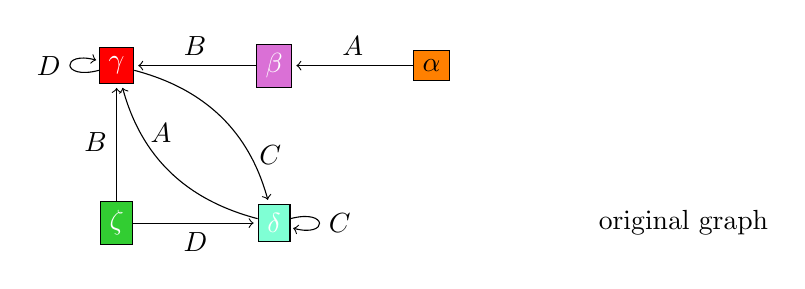
\begin{tikzpicture}[scale=1]       % initial graph
    \node[draw, fill=orange] at (4, 2) (start) {$\alpha$};
    \node[draw,fill=Orchid,text=white] at (2, 2) (K) {$\beta$};
    \node[draw,fill=red,text=white] at (0, 2) (R) {$\gamma$};
    \node[draw,fill=LimeGreen,text=white] at (0, 0) (G) {$\zeta$};
    \node[draw,fill=Aquamarine,text=white] at (2, 0) (B) {$\delta$};
    
    \draw (start) edge[->] node[above] {$A$} (K);
    \draw (K) edge[->] node[above] {$B$} (R);
    \draw (B) edge[->, loop right] node {$C$} ();
    \draw (B) edge[->, bend left] node[right, near end] {$A$} (R);
    \draw (G) edge[->] node[below] {$D$} (B);

    \draw (R) edge[->, loop left] node {$D$} ();
    \draw (G) edge[->] node[left] {$B$} (R);
    \draw (R) edge[->, bend left] node[right, near end] {$C$} (B);

    \node[anchor=west] at (6, 0) {original graph};
  \end{tikzpicture}

  \vspace{0.25cm}
  \hrule
  \vspace{0.25cm}

  
  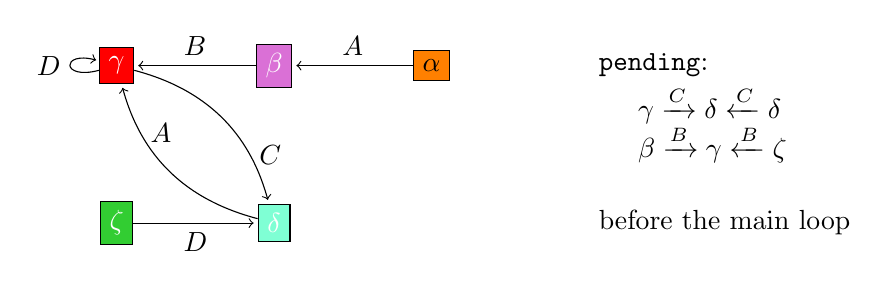
\begin{tikzpicture}[scale=1]       % STEP 0
    \node[draw, fill=orange] at (4, 2) (start) {$\alpha$};
    \node[draw,fill=Orchid,text=white] at (2, 2) (K) {$\beta$};
    \node[draw,fill=red,text=white] at (0, 2) (R) {$\gamma$};
    \node[draw,fill=LimeGreen,text=white] at (0, 0) (G) {$\zeta$};
    \node[draw,fill=Aquamarine,text=white] at (2, 0) (B) {$\delta$};
    
    \draw (start) edge[->] node[above] {$A$} (K);
    \draw (K) edge[->] node[above] {$B$} (R);
    % not hot \draw (B) edge[->, loop right] node {$C$} ();
    \draw (B) edge[->, bend left] node[right, near end] {$A$} (R);
    \draw (G) edge[->] node[below] {$D$} (B);

    \draw (R) edge[->, loop left] node {$D$} ();
% not hot    \draw (G) edge[->] node[left] {$B$} (R);
    \draw (R) edge[->, bend left] node[right, near end] {$C$} (B);

    \node[anchor=west] at (6, 2) {\texttt{pending}:};
    \node[anchor=west] at (6.5, 1) {$\beta \xrightarrow{B} \gamma \xleftarrow{B} \zeta$};
    \node[anchor=west] at (6.5, 1.5) {$\gamma \xrightarrow{C} \delta \xleftarrow{C} \delta$};
    \node[anchor=west] at (6, 0) {before the main loop};

  \end{tikzpicture}

  \vspace{0.25cm}
  \hrule
  \vspace{0.25cm}
  
  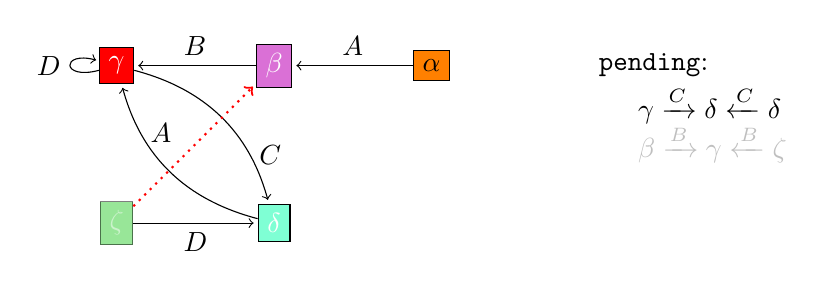
\begin{tikzpicture}[scale=1]      % STEP 1
    \node[draw, fill=orange] at (4, 2) (start) {$\alpha$};
    \node[draw,fill=Orchid,text=white] at (2, 2) (K) {$\beta$};
    \node[draw,fill=red,text=white] at (0, 2) (R) {$\gamma$};
    \node[draw,semitransparent,fill=LimeGreen,text=white] at (0, 0) (G) {$\zeta$};
    \node[draw,fill=Aquamarine,text=white] at (2, 0) (B) {$\delta$};
    
    \draw (start) edge[->] node[above] {$A$} (K);
    \draw (K) edge[->] node[above] {$B$} (R);
    \draw (B) edge[->, bend left] node[right, near end] {$A$} (R);
    \draw (G) edge[->] node[below] {$D$} (B);

    \draw (R) edge[->, loop left] node {$D$} ();
    \draw (R) edge[->, bend left] node[right, near end] {$C$} (B);

    \draw (G) edge[->, red, thick, dotted] (K);
 
    % labels à droite
    \node[anchor=west] at (6, 2) {\texttt{pending}:};
    \node[anchor=west, lightgray] at (6.5, 1) {$\beta \xrightarrow{B} \gamma \xleftarrow{B} \zeta$};
    \node[anchor=west] at (6.5, 1.5) {$\gamma \xrightarrow{C} \delta \xleftarrow{C} \delta$};
  \end{tikzpicture}

  \vspace{0.25cm}
  \hrule
  \vspace{0.25cm}
  
  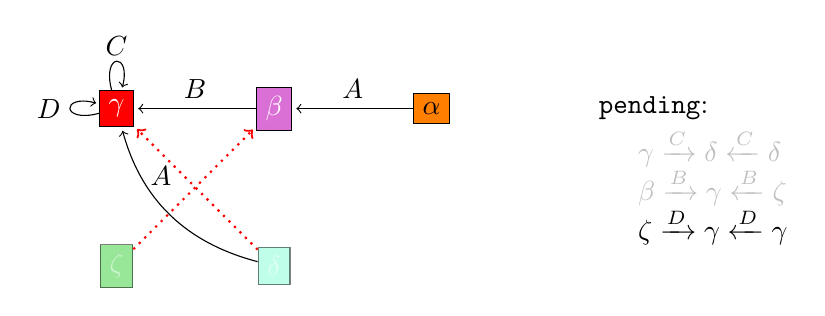
\begin{tikzpicture}[scale=1]      % STEP 2
    \node[draw, fill=orange] at (4, 2) (start) {$\alpha$};
    \node[draw,fill=Orchid,text=white] at (2, 2) (K) {$\beta$};
    \node[draw,fill=red,text=white] at (0, 2) (R) {$\gamma$};
    \node[draw,semitransparent,fill=LimeGreen,text=white] at (0, 0) (G) {$\zeta$};
    \node[draw,semitransparent,fill=Aquamarine,text=white] at (2, 0) (B) {$\delta$};

    \draw (start) edge[->] node[above] {$A$} (K);
    \draw (K) edge[->] node[above] {$B$} (R);
    \draw (R) edge[->, loop above] node[above=-0.5mm] {$C$} ();
    \draw (B) edge[->, bend left] node[right, near end] {$A$} (R);
    \draw (R) edge[->, loop left] node {$D$} ();
    \draw (G) edge[->, red, thick, dotted] (K);
    \draw (B) edge[->, red, thick, dotted] (R);

    % labels à droite
    \node[anchor=west] at (6, 2) {\texttt{pending}:};
    \node[anchor=west, lightgray] at (6.5, 1) {$\beta \xrightarrow{B} \gamma \xleftarrow{B} \zeta$};
    \node[anchor=west, lightgray] at (6.5, 1.5) {$\gamma \xrightarrow{C} \delta \xleftarrow{C} \delta$};
    \node[anchor=west] at (6.5, 0.5) {$\zeta \xrightarrow{D} \gamma \xleftarrow{D} \gamma$};
  \end{tikzpicture}

  \vspace{0.25cm}
  \hrule
  \vspace{0.25cm}
  
  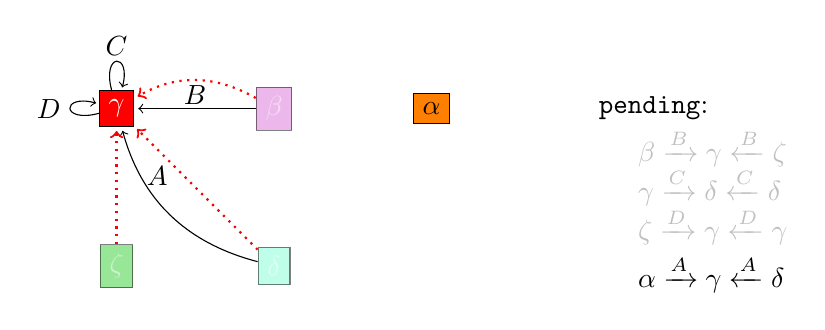
\begin{tikzpicture}[scale=1]      % STEP 3
    \node[draw, fill=orange] at (4, 2) (start) {$\alpha$};
    \node[draw,semitransparent,fill=Orchid,text=white] at (2, 2) (K) {$\beta$};
    \node[draw,fill=red,text=white] at (0, 2) (R) {$\gamma$};
    \node[draw,semitransparent,fill=LimeGreen,text=white] at (0, 0) (G) {$\zeta$};
    \node[draw,semitransparent,fill=Aquamarine,text=white] at (2, 0) (B) {$\delta$};

    \draw (K) edge[->] node[above=-0.75mm] {$B$} (R);
    \draw (R) edge[->, loop above] node[above=-0.5mm] {$C$} ();
    \draw (B) edge[->, bend left] node[right=-0.5mm, near end] {$A$} (R);
    \draw (R) edge[->, loop left] node {$D$} ();
    \draw (G) edge[->, red, thick, dotted] (R);
    \draw (B) edge[->, red, thick, dotted] (R);
    \draw (K) edge[->, red, thick, dotted, bend right] (R);
     
    % labels à droite
    \node[anchor=west] at (6, 2) {\texttt{pending}:};
    \node[anchor=west, lightgray] at (6.5, 1.5) {$\beta \xrightarrow{B} \gamma \xleftarrow{B} \zeta$};
    \node[anchor=west, lightgray] at (6.5, 1) {$\gamma \xrightarrow{C} \delta \xleftarrow{C} \delta$};
    \node[anchor=west, lightgray] at (6.5, 0.5) {$\zeta \xrightarrow{D} \gamma \xleftarrow{D} \gamma$};
    \node[anchor=west] at (6.5, -0.1) {$\alpha \xrightarrow{A} \gamma \xleftarrow{A} \delta$};
  \end{tikzpicture}

  \vspace{0.25cm}
  \hrule
  %\vspace{0.25cm}
  
  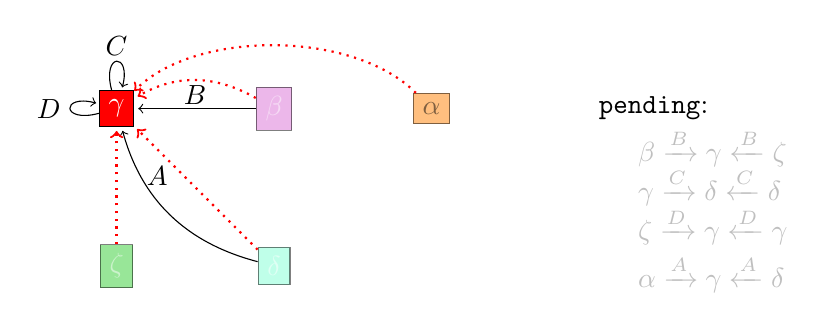
\begin{tikzpicture}[scale=1]      % STEP 4
    \node[draw,semitransparent,fill=orange] at (4, 2) (start) {$\alpha$};
    \node[draw,semitransparent,fill=Orchid,text=white] at (2, 2) (K) {$\beta$};
    \node[draw,fill=red,text=white] at (0, 2) (R) {$\gamma$};
    \node[draw,semitransparent,fill=LimeGreen,text=white] at (0, 0) (G) {$\zeta$};
    \node[draw,semitransparent,fill=Aquamarine,text=white] at (2, 0) (B) {$\delta$};

    \draw (K) edge[->] node[above=-0.75mm] {$B$} (R);

    \draw (R) edge[->, loop above] node[above=-0.5mm] {$C$} ();

    \draw (B) edge[->, bend left] node[right=-0.5mm, near end] {$A$} (R);    
    \draw (R) edge[->, loop left] node {$D$} ();
    \draw (G) edge[->, red, thick, dotted] (R);
    \draw (B) edge[->, red, thick, dotted] (R);
    \draw (K) edge[->, red, thick, dotted, bend right] (R);
    \draw[->, red, thick, dotted] (start) .. controls (3, 3) and (1, 3) .. (R);      
     
    % labels à droite
    \node[anchor=west] at (6, 2) {\texttt{pending}:};
    \node[anchor=west, lightgray] at (6.5, 1.5) {$\beta \xrightarrow{B} \gamma \xleftarrow{B} \zeta$};
    \node[anchor=west, lightgray] at (6.5, 1) {$\gamma \xrightarrow{C} \delta \xleftarrow{C} \delta$};
    \node[anchor=west, lightgray] at (6.5, 0.5) {$\zeta \xrightarrow{D} \gamma \xleftarrow{D} \gamma$};
    \node[anchor=west, lightgray] at (6.5, -0.1) {$\alpha \xrightarrow{A} \gamma \xleftarrow{A} \delta$};
  \end{tikzpicture}
\end{center}

\caption{Step-by-step illustration of Algorithm~\ref{algo:main-dense}. The plain
  edges are ``hot''. The dotted edges represent the supernode leaders (for
  non-trivial supernodes). \label{fig:step-by-step}}
\end{figure}

It is clear that \textsc{AddEdge} runs in constant time, and that \textsc{Merge}
runs in $\bigO{B}$ operations.  The setup phase of \textsc{CollapseMaze}
requires $\bigO{WB + E}$ operations. The number of iterations of the
\textbf{while} loop is at most $E$ (each new wormhole added to \texttt{pending}
destroys an edge). \textsc{Merge} can only be invoked $W-1$ times. So the total
time spent in \textsc{Merge} is $\bigO{BW}$ and the total time spent in calls to
\textsc{Find} is $\bigO{E \alpha(W)}$, where $\alpha$ is the inverse-Ackermann
function (thanks to the celebrated amortized analysis
of~\cite{10.1145/62.2160}). Note that $\alpha(W)$ is upper-bounded by 4 when its
$W$ is less than the number of atoms in the universe. So, the final complexity
of \textsc{CollapseMazeDense} is $\bigO{BW + E \alpha(W)}$.

$E \approx W^2$ and $W \approx B$, then this gives a nearly-quadratic algorithm,
improving upon the known cubic one.

\subsection{Sparse mazes}
\label{sec:sparse}

When $E$ is much less than $BW$, several aspects of the algorithm could be made
more efficient. For instance, \textsc{Merge} requires $B$ operations to inspect
$B$ potential edges, even if just a few are present. We can use a lightweight
variant of the ``sparse array'' technique abundantly used in very early sparse
matrix codes and rediscovered 20 years later~\cite{10.1145/176454.176484} in a
different context. To efficiently iterate on the hot incoming edges to a node,
we also use an auxiliary array \texttt{hotbox} where $\texttt{hotbox}[\omega]$
contains a list of $X$'s such that $\texttt{hot}[\omega, X] \neq \texttt{none}$.

Also, when merging two nodes, we could absorb the ``smaller'' one (with less
edges to process) into the ``larger'' one. Doing all the work on the smaller of
the two nodes minimizes the total amount of work (this idea is common ; for
instance it is at work in Hopcroft's DFA minimization
algorithm~\cite{hopcroft1971nlogn}). Unfortunately, this breaks down the
guarantees offered by the disjoint set data structure. We therefore make do with
a more naive solution: we eagerly update all nodes when two sets are joined.

All nodes have a pointer (\texttt{leader}) to the leader node in their supernode
(possibly themselves). Supernode leaders have a list (\texttt{followers}) of
nodes in their supernode. The \emph{size} of a (super)node is the number of
nodes it contains plus the number of incoming edges. The algorithm maintains the
sizes at all time (in an array \texttt{size}), as new wormholes are discovered
and (super)nodes are merged. When two (super)nodes are merged, to form the
resulting supernode, the smaller one (by \texttt{size}) is ``absorbed'' into the
larger one. More precisely:
\begin{itemize}
\item The \texttt{leader} pointer of all nodes in the smaller (super)node is set to the
  larger supernode.
\item Hot edges pointing to the smaller supernode either create a wormhole and
  are dropped, or become hot edges pointing to the larger supernode.
\item The size of the larger supernode is augmented accordingly.
\end{itemize}



\begin{algorithm}
\begin{algorithmic}[1]
  % an edge either becomes hot or creates a wormhole
  \Procedure{AddEdge'}{$\alpha, X, i, \beta$}
   \If{$\texttt{hot}[\beta, X] = \texttt{some} (\gamma, j)$}
   \State $\texttt{pending} \gets (\alpha, X, i, \beta, j, \gamma)) :: \texttt{pending}$       \Comment{detected $\alpha \xrightarrow{X.i} \beta \xleftarrow{X.j} \gamma$}
   \Else
   \State $\texttt{hot}[\beta, X] \gets \texttt{some} (\alpha, i)$   
   \State $\texttt{hotbox}[\beta] \gets X :: \texttt{hotbox}[\beta]$    \Comment{Register non-empty location}
   \EndIf
   \EndProcedure

  \bigskip

  \Procedure{Merge'}{$\sigma, \pi$}                                    
  \If{$\texttt{size}[\sigma] > \texttt{size}[\pi]$}                   
  \State $\texttt{tmp} \gets \sigma, \sigma \gets \pi, \pi \gets \texttt{tmp}$  \Comment{union-by-size: now $\texttt{size}[\sigma] \leq \texttt{size}[\pi]$}
  \EndIf

  \State $\texttt{size}[\pi] \gets \texttt{size}[\pi] + \texttt{size}[\sigma]$
  
  \For{each $\omega \in \texttt{followers}[\sigma]$}                             
  \State $\texttt{leader}[\omega] \gets \pi$                               
  \State $\texttt{followers}[\pi] \gets \omega :: \texttt{followers}[\pi]$ 
  \EndFor

  \For{each $X \in \texttt{hotbox}[\sigma]$}                          \Comment{sparse iteration}       
  \State $\texttt{some} (\omega, i) \gets \texttt{hot}[\sigma, X]$    \Comment{looking at $\omega \xrightarrow{X.i} \sigma$}
  \State $\Call{AddEdge'}{\omega, X, i, \pi}$                          \Comment{replace by $\omega \xrightarrow{X.i} \pi$}
  \EndFor  
  \EndProcedure

  \bigskip

  \Procedure{CollapseMazeSparse}{$W, B, \texttt{G}$}                          
  \State $\texttt{pending} \gets \texttt{[]}$                           \Comment{Setup}
  \For{$0 \leq \alpha < W$}
    \State $\texttt{size}[\alpha] \gets 1$
    \State $\texttt{leader}[\alpha] \gets \alpha$                       \Comment{$\alpha$ is a supernode by itself}
    \State $\texttt{followers}[\alpha] \gets \alpha :: \texttt{[]}$
    \State $\texttt{hotbox}[\alpha] \gets \texttt{[]}$                 
    \For{$0 \leq X < B$}
    \State $\texttt{hot}[\alpha,X] \gets \texttt{none}$                 \Comment{potential \texttt{hot}-spot}
    \EndFor
    \For{each $(X, i, \beta)$ in $\texttt{G}[\alpha]$}                  \Comment{prime the wormhole pump} 
      \State $\Call{AddEdge'}{\alpha, X, i, \beta}$
      \State increment $\texttt{size}[\beta]$
    \EndFor
  \EndFor

  \While{$\texttt{pending} \neq \texttt{[]}$}                                  \Comment{main loop : process known wormholes}
  \State $(\alpha, X, i, \beta, j, \gamma) :: \texttt{tail} \gets \texttt{pending}$     \Comment{popped $\alpha \xrightarrow{X.i} \beta \xleftarrow{X.j} \gamma$}
  \State $\texttt{pending} \gets \texttt{tail}$    
  \If{$\texttt{leader}[\alpha] \neq \texttt{leader}[\gamma]$}                   \Comment{already merged?}
  \State $\Call{Merge'}{\texttt{leader}[\alpha], \texttt{leader}[\gamma]}$       \Comment{merge nodes containing $\alpha$ and $\gamma$}                            
  \EndIf
  \EndWhile
  \EndProcedure
\end{algorithmic}
\caption{Algorithm to collapse sparse recursive mazes. \label{algo:main-sparse}}
\end{algorithm}

\textsc{AddEdge'} still runs in constant time, and \textsc{Merge}
runs in time dominated by the \texttt{size} of the smaller supernode: it takes
constant-time per wire in the smaller supernode, plus constant time per hot edge
pointing to the smaller supernode (thanks to the \texttt{hotbox} array)---and
not all edges are hot, hence the upper-bound.

% \textsc{Find} runs in time $\bigO{W}$ in the worst-case (it may go through all
% wires), however it follows from~\cite[Thm. 4]{10.1145/62.2160} that each
% \textsc{Find} operation terminates in amortized time $\bigO{\log W}$, because we
% use path compression.

The number of iterations of the \textbf{while} loop is again at most $E$ and it
does a constant number of operation per iteration, excluding calls to
\textsc{Merge}. It thus remains to control the total time spent in
\textsc{Merge}---and this is the tricky part. As the algorithm progresses, the
sequence of merges can be represented by a binary forest. The wires of the maze
are the leaves, and each call to \textsc{Merge} creates a new root whose two
children are preexisting roots. It represents a new supernode containing all the
wires associated to the leaves in the subtree. Each supernode is labelled by its
size (as defined above). When two roots of labels $x \leq y$ are joined, the
result has label $x + y$, and we are ``charged'' $x$ operations (the smaller
size).

In the example detailed in Fig.~\ref{fig:step-by-step}, this forest is in fact a
binary tree:
\begin{center}
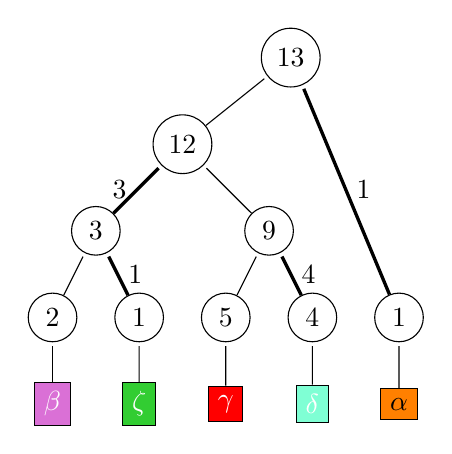
\begin{tikzpicture}[scale=0.55]
  \node[draw,fill=Orchid,text=white]     at (0, -2) (K) {$\beta$};
  \node[draw,fill=LimeGreen,text=white]  at (2, -2) (G) {$\zeta$};
  \node[draw,fill=red,text=white]        at (4, -2) (R) {$\gamma$};
  \node[draw,fill=Aquamarine,text=white] at (6, -2) (B) {$\delta$};
  \node[draw, fill=orange]               at (8, -2) (start) {$\alpha$};

  \node[draw,circle] at (0, 0) (K2) {2};
  \node[draw,circle] at (2, 0) (G2) {1};
  \node[draw,circle] at (4, 0) (R2) {5};
  \node[draw,circle] at (6, 0) (B2) {4};
  \node[draw,circle] at (8, 0) (start2) {1};
  
  \node[draw,circle] at (1, 2)  (foo) {3};
  \node[draw,circle] at (5, 2)  (bar) {9};
  \node[draw,circle] at (3, 4)  (foobar) {12};
  \node[draw,circle] at (5.5, 6) (root) {13};

  \draw (K) edge (K2);
  \draw (B) edge (B2);
  \draw (G) edge (G2);
  \draw (R) edge (R2);
  \draw (start) edge (start2);
  
  \draw (K2) edge (foo);
  \draw (G2) edge[very thick] node[right] {1} (foo);
  \draw (B2) edge[very thick] node[right] {4} (bar);
  \draw (R2) edge (bar);
  \draw (foo) edge[very thick] node[left] {3} (foobar);
  \draw (bar) edge (foobar);
  \draw (foobar) edge (root);
  \draw (start2) edge[very thick] node[right] {1} (root);
\end{tikzpicture}
\end{center}

Let $\mathcal{F}$ denote an arbitrary merge forest built from the dual
representation graph of a recursive maze. Its $W$ leaves are labelled with the
size of the wires (one plus the number of incoming edges). Let $S$ denote the
sum of sizes: if the dual representation graph has $E$ edges, then
$S \leq W + E$.  Let $C(\mathcal{F})$ denote the total amount ``charged'' by
this merge forest (i.e., an upper-bound on the total number of operations spent
in \textsc{Merge} during the process). Then we have:

\medskip

\begin{lemma}
  $C(\mathcal{F}) \leq S \log_2 S$.
\end{lemma}

\begin{proof}  
  Let $t_\omega$ denote the number of times the supernode containing wire
  $\omega$ is absorbed into a larger supernode in $\mathcal{F}$ (this counts the
  number of times $\omega$ belongs to the smallest of two sets being joined). By
  definition,
  \[
    C(\mathcal{F}) \leq \sum_{\omega \in \mathcal{W}} \texttt{size}[\omega] \times t_\omega.
  \]
  Our plan is to upper-bound the $t_\omega$'s. Because of the union-by-size
  rule, each time the supernode containing $\omega$ is the smaller of the two,
  the size of new supernode created by the merge is at least twice as large. If
  follows that the root containing $\omega$ must have size at least
  $\texttt{size}[\omega] 2^{t_\omega}$. Because this cannot be greater than $S$,
  it follows that $t_\omega \leq \log_2 (S / \texttt{size}[\omega])$. We
  conclude that
  \[
    C(\mathcal{F}) \leq \sum_{\omega \in \mathcal{W}} \texttt{size}[\omega] \times \log_2 \frac{E}{\texttt{size}[\omega]}
  \]
  and the lemma is proved because $S = \sum_\omega \texttt{size}[\omega]$.
\end{proof}

Therefore, the total running time of \textsc{CollapseMazeSparse} is
$\bigO{BW + E \log E}$. At first glance, this could seem like a
\emph{decremental} improvement compared to \textsc{CollapseMazeDense}. However,
the \emph{only} part that requires $BW$ operations is the initialization of the
$\texttt{hot}$ array. We therefore see two ways to cheat our way out of this
embarrassing situation.

\begin{itemize}
\item We initially need the \texttt{hot} array to be filled with the
  \texttt{none} value. If the array was \emph{provided} to us in this state,
  then everything would be perfect. \textsc{CollapseMazeSparse} would run in
  time $\bigO{E \log E}$, mission accomplished. And although this is \emph{a
    bit} cheating, it is not too bad because we could easily \emph{restore} the
  \texttt{hot} array to its initial state with only a constant factor increase
  in the running time (just store the indices of all modified locations and
  restore them to \texttt{none} at the end of the algorithm).

  It follows that if a long sequence of mazes had to be solved in sequence, then
  a single (large enough) \texttt{hot} array could be initialized \emph{once}
  and used several times, so the cost of its initialization could be amortized
  over an (arbitrarily long) sequence of uses.

\item Initializing the \texttt{hot} array annoys us. Wo we could simply get rid
  of it and use a hash table instead. It will ever only hold $E$ entries, and we
  have a time budget to initialize an array of size $E \log E$, so that we can
  keep the fill ratio of this hash table comfortably low.  However, this
  requires some kind of randomization and we leave it as an open problem.
\end{itemize}


\section{Construction of an exit path}
\label{sec:arg}

All wires in an equivalence class of $\stackrel{*}{\equiv}$ are mutually
reachable (without modifying the stack). In this section we show how to augment
Algorithms~\ref{algo:main-dense} and~\ref{algo:main-sparse} to provide the
computation of such paths without asymptotically increasing their complexity.

In dual representation graph, an edge $\alpha \xrightarrow{X.i} \beta$ is
labelled with an instruction (``$X.i$''). This describes a feasible move in the
maze (and a valid transition in the pushdown automaton that pushes $X$).

We extend this as follows: each edge is labelled with a \emph{box attribute}
($X$---what recursive box is entered by taking this edge) and the
\emph{identifier of an instruction sequence} (that describes what must be done
to actually cross the edge). We write these identifier with a ``sharp''
(e.g. \#42). There is also a global \emph{context} that maps instruction
sequence identifiers to actual sequences of instructions and instruction
sequence identifiers. This time, an edge $\alpha \xrightarrow[\#42]{X} \beta$
means that the sequence of instruction $\#42$ takes the player from wire
$\alpha$ to wire $\beta$, while entering box $X$. So, before the graph rewriting
process even start, we transform the dual representation graph into the
\emph{extended dual representation graph} shown in Fig.~\ref{fig:extended}.

We then perform the same graph rewriting process, except that we now take care
of instruction sequence identifiers as shown in
Fig.~\ref{fig:merge-extended}. All the edges incident to the supernode that gets
``absorbed'' gets a new instruction sequence identifier. In the figure, the
sequence of instruction $\# \mathcal{K} := \mathcal{I} ; \overline{\mathcal{J}}$
travels from $\alpha$ to $\gamma$. Edges incoming into $\alpha$ are now incoming
into $\gamma$, therefore $\# \mathcal{K}$ must be added after their instruction
sequence. Edges pointing out of $\alpha$ now point out of $\gamma$, so
$\overline{\# \mathcal{K}}$ must be added before their instruction sequence. We
finally record the ``spanning'' edge
$\alpha \xrightarrow{\# \mathcal{K}} \gamma$.

\begin{figure}
\begin{center}
  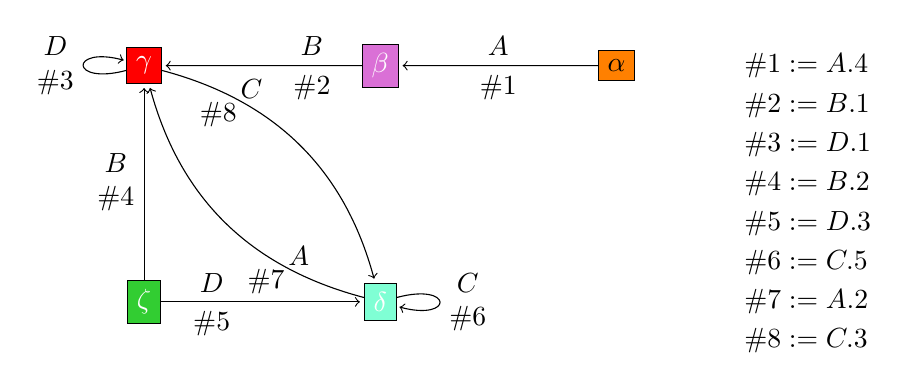
\begin{tikzpicture}[scale=1.5]
    \node[draw,fill=red,text=white] at (0, 2) (R) {$\gamma$};
    \node[draw,fill=LimeGreen,text=white] at (0, 0) (G) {$\zeta$};
    \node[draw,fill=Aquamarine,text=white] at (2, 0) (B) {$\delta$};
    \node[draw,fill=Orchid,text=white] at (2, 2) (K) {$\beta$};
    \node[draw, fill=orange] at (4, 2) (start) {$\alpha$};
    
    \draw (start) edge[->] node[above] {$A$} node[below] {\#1} (K);
    \draw (K) edge[->] node[above, near start] {$B$} node[below, near start] {\#2} (R);

    \draw (B) edge[->, loop right] node[right,align=center] {$C$ \\ $\#6$} ();
    \draw (B) edge[->, bend left] node[near start, below left=-1mm] {$\#7$} node[near start, above right=-1mm] {$A$} (R);

    \draw (G) edge[->] node[above, near start] {$D$} node[below, near start] {$\#5$} (B);
    \draw (G) edge[->] node[left,align=center] {$B$ \\ $\#4$} (R);
    
    \draw (R) edge[->, loop left] node[left,align=center] {$D$ \\ $\#3$} ();

    \draw (R) edge[->, bend left] node[near start, above right=-1mm] {$C$} node[near start, below left=-1mm] {$\#8$} (B);

    \node[anchor=west] at (5, 2)    {$\#1 := A.4$};
    \node[anchor=west] at (5, 1.66) {$\#2 := B.1$};
    \node[anchor=west] at (5, 1.33) {$\#3 := D.1$};
    \node[anchor=west] at (5, 1)    {$\#4 := B.2$};
    \node[anchor=west] at (5, 0.66) {$\#5 := D.3$};
    \node[anchor=west] at (5, 0.33) {$\#6 := C.5$};
    \node[anchor=west] at (5, 0)    {$\#7 := A.2$};
    \node[anchor=west] at (5,-0.33) {$\#8 := C.3$};
  \end{tikzpicture}
\end{center}
\caption{\label{fig:extended} Extended dual representation graph corresponding to the simple maze of Fig.~\ref{fig:simple}.}
\end{figure}



\begin{figure}
\centering
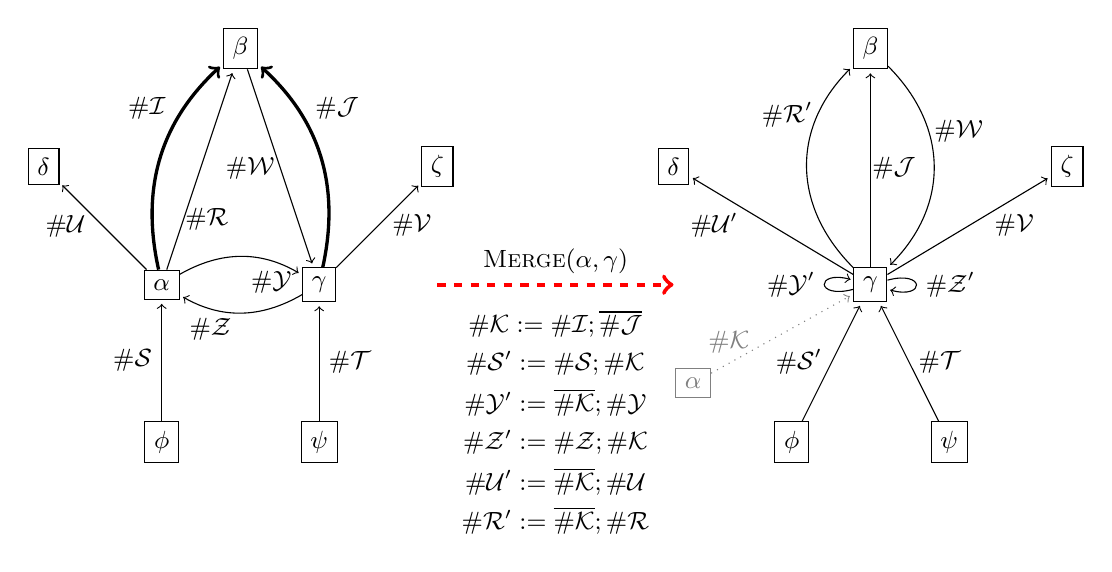
\begin{tikzpicture}[every node/.style={font=\small}, every edge/.style={draw,shorten >=0.5mm}]
  \begin{scope}
  \node[draw] at (0, 0) (a) {$\alpha$};
  \node[draw] at (2, 0) (c) {$\gamma$};
  \node[draw] at (1, 3) (b) {$\beta$};
  \node[draw] at (-1.5, 1.5) (d) {$\delta$};
  \node[draw] at (3.5, 1.5) (e) {$\zeta$};
  \node[draw] at (0, -2) (f) {$\phi$};
  \node[draw] at (2, -2) (g) {$\psi$};

  \draw (a) edge[->,very thick, bend left] node[left=1mm, near end]   {$\# \mathcal{I}$} (b);
  \draw (c) edge[->,very thick, bend right] node[right=1mm, near end] {$\# \mathcal{J}$} (b);
  \draw (a) edge[->,bend left] node[below, near end] {$\# \mathcal{Y}$} (c);
  \draw (c) edge[->,bend left] node[below, near end] {$\# \mathcal{Z}$} (a);
  \draw (a) edge[->] node[right=-1mm, near start]    {$\# \mathcal{R}$} (b);
  \draw (a) edge[->] node[left=1mm]                  {$\# \mathcal{U}$} (d);
  \draw (b) edge[->] node[left=-0.5mm]               {$\# \mathcal{W}$} (c);
  \draw (c) edge[->] node[right=0.5mm]               {$\# \mathcal{V}$} (e);
  \draw (f) edge[->] node[left]                      {$\# \mathcal{S}$} (a);
  \draw (g) edge[->] node[right]                     {$\# \mathcal{T}$} (c);
\end{scope}

\draw[ultra thick, red, dashed, ->] (3.5, 0) -- node[black,above] {\textsc{Merge}$(\alpha, \gamma)$} (6.5, 0);

\begin{scope}[xshift=8cm]
  \node[draw, gray] at (-1.25, -1.25) (a) {$\alpha$};

  \node[draw] at (1, 0) (ac) {$\gamma$};
  \node[draw] at (1, 3) (b) {$\beta$};
  \node[draw] at (-1.5, 1.5) (d) {$\delta$};
  \node[draw] at (3.5, 1.5) (e) {$\zeta$};
  \node[draw] at (0, -2) (f) {$\phi$};
  \node[draw] at (2, -2) (g) {$\psi$};

  \draw[->,shorten >=0.5mm] (ac) .. controls (0, 1) and (0, 2) .. node[left=-0.5mm, near end] {$\# \mathcal{R}'$}  (b);
  \draw[->,shorten >=0.5mm] (b)  .. controls (2, 2) and (2, 1) .. node[right=-0.5mm, pos=0.33] {$\# \mathcal{W}$} (ac);

  \draw (ac) edge[->,loop left] node[left]                 {$\# \mathcal{Y}'$} (ac);
  \draw (ac) edge[->,loop right] node[right]               {$\# \mathcal{Z}'$} (ac);
  \draw (ac) edge[->] node[right=-1mm]                     {$\# \mathcal{J}$}  (b);
  \draw (ac) edge[->] node[left=3mm]                       {$\# \mathcal{U}'$} (d);
  \draw (ac) edge[->] node[right=2mm]                      {$\# \mathcal{V}$}  (e);
  \draw (f) edge[->] node[left]                            {$\# \mathcal{S}'$} (ac);
  \draw (g) edge[->] node[right]                           {$\# \mathcal{T}$}  (ac);
  \draw[gray, dotted] (a) edge[->] node[above, very near start] {$\# \mathcal{K}$}  (ac);

\end{scope}

\node at (5, -0.5) {$\# \mathcal{K}  := \# \mathcal{I}            ; \overline{\# \mathcal{J}}$};
\node at (5, -1.0) {$\# \mathcal{S}' := \# \mathcal{S}            ; \# \mathcal{K}$};
\node at (5, -1.5) {$\# \mathcal{Y}' := \overline{\# \mathcal{K}}; \# \mathcal{Y}$};
\node at (5, -2.0) {$\# \mathcal{Z}' := \# \mathcal{Z}            ; \# \mathcal{K}$};
\node at (5, -2.5) {$\# \mathcal{U}' := \overline{\# \mathcal{K}}; \# \mathcal{U}$};
\node at (5, -3.0) {$\# \mathcal{R}' := \overline{\# \mathcal{K}}; \# \mathcal{R}$};

\end{tikzpicture}
\caption{\label{fig:merge-extended} Illustration of the extended graph contraction
  process (showing only instruction sequence identifiers). The two thick edges
  have the same box attribute. It modifies the labels of all edges incident to
  $\alpha$ and registers one new instruction sequence identifier for each one.}
\end{figure}

We the rewriting process is over, the spanning edge form (rooted) spanning trees
of the connected components. Therefore, when a pair of nodes are reachable by a
path, this path can be assembled by following the spanning edges.

Compared to Algorithms~\ref{algo:main-dense} and~\ref{algo:main-sparse}, this
requires the following modifications:
\begin{itemize}
\item Not only the target, but also the origin of hot edges incident to an
  ``absorbed'' node must be modified. This requires each node to we aware not
  only of its incoming hot edges, but also of the outgoing ones.

\item The instruction sequences on each edge must be maintained.

\item When a wormhole
  $\alpha \xrightarrow[\# \mathcal{I}]{X} \beta \xleftarrow[\# \mathcal{J}]{X}
  \gamma$ is discovered, one of the two edges is removed from the graph, but its
  instruction sequence identifier must not be lost (otherwise we will not be
  able to form the spanning edge). Therefore,
  $(\alpha, X, \# \mathcal{I}, \beta, \# \mathcal{J}, \gamma)$ must be pushed
  onto the \texttt{pending} list.

\item Spanning edges must be stored separately.
\end{itemize}

Fig.~\ref{fig:path-finding} illustrates the process. In the end, this produces the path \#18, that expands as:
\begin{align*}
  \#18
  &= \# 16; \overline{\#14} \\
  &= (A.4; \#15); (\overline{A.2}; \#11) \\
  &= A.4; (\#12; \overline{D.1}); \overline{A.2}; (C.5; \overline{C.3});  \\
  &= A.4; (\#10; \#11); \overline{D.1}; \overline{A.2}; C.5; \overline{C.3} \\
  &= A.4; (\overline{\#9}; D.3); (C.5; \overline{C.3}); \overline{D.1}; \overline{A.2}; C.5; \overline{C.3} \\
  &= A.4; B.1; \overline{B.2}; D.3; C.5; \overline{C.3}; \overline{D.1}; \overline{A.2}; C.5; \overline{C.3}
\end{align*}
This is indeed an exit path, but not one of optimal length (compare to the one
given earlier in the text). Note that exponentially-long paths can be
represented in polynomial space by the list of instruction sequence identifiers.

We leave the problem of producing a minimal-length exit path open for future work.

%%%%%%%%%%%%%%%%%%%%%%%%%%%%%%%%%%%%%%%%%%%%%%%%%%%%%%%%%%%%%%%%%%%%%%%%%%%%%%

\begin{figure}
\begin{center}
  \tikzset{every node/.style={font=\scriptsize}}

  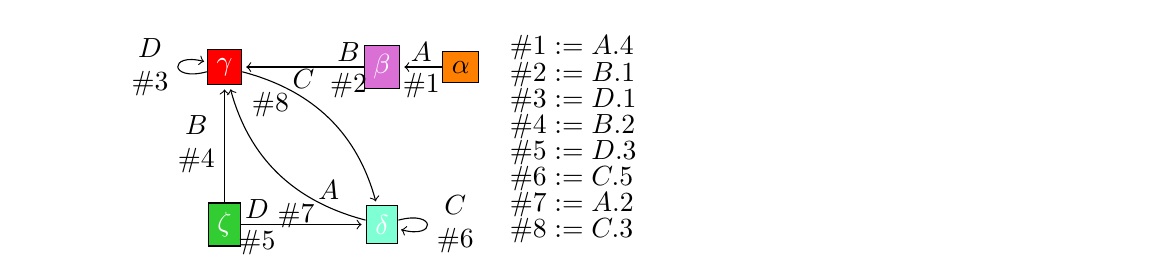
\begin{tikzpicture}[scale=1]       % initial graph
    \path[use as bounding box] (-2.5, -0.25) rectangle (11.5, 2.5);

    \node[draw,fill=red,text=white] at (0, 2) (R) {$\gamma$};
    \node[draw,fill=LimeGreen,text=white] at (0, 0) (G) {$\zeta$};
    \node[draw,fill=Aquamarine,text=white] at (2, 0) (B) {$\delta$};
    \node[draw,fill=Orchid,text=white] at (2, 2) (K) {$\beta$};
    \node[draw, fill=orange] at (3, 2) (start) {$\alpha$};
    
    \draw (start) edge[->] node[above=-0.5mm] {$A$} node[below=-0.5mm] {\#1} (K);
    \draw (K) edge[->] node[above=-0.5mm, very near start] {$B$} node[below=-0.5mm, very near start] {\#2} (R);

    \draw (B) edge[->, loop right] node[right,align=center] {$C$ \\ $\#6$} ();
    \draw (B) edge[->, bend left] node[near start, below left=-1mm] {$\#7$} node[near start, above right=-1mm] {$A$} (R);

    \draw (G) edge[->] node[above=-0.5mm, very near start] {$D$} node[below=-0.5mm, very near start] {$\#5$} (B);
    \draw (G) edge[->] node[left,align=center] {$B$ \\ $\#4$} (R);
    
    \draw (R) edge[->, loop left] node[left,align=center] {$D$ \\ $\#3$} ();

    \draw (R) edge[->, bend left] node[near start, above right=-1mm] {$C$} node[near start, below left=-1mm] {$\#8$} (B);

    \begin{scope}[xshift=-1.5cm,yshift=0.25cm]
    \node[anchor=west] at (5, 2)    {$\#1 := A.4$};
    \node[anchor=west] at (5, 1.66) {$\#2 := B.1$};
    \node[anchor=west] at (5, 1.33) {$\#3 := D.1$};
    \node[anchor=west] at (5, 1)    {$\#4 := B.2$};
    \node[anchor=west] at (5, 0.66) {$\#5 := D.3$};
    \node[anchor=west] at (5, 0.33) {$\#6 := C.5$};
    \node[anchor=west] at (5, 0)    {$\#7 := A.2$};
    \node[anchor=west] at (5,-0.33) {$\#8 := C.3$};
  \end{scope}
\end{tikzpicture}

  \vspace{0.25cm}
  \hrule
  \vspace{0.25cm}

  
  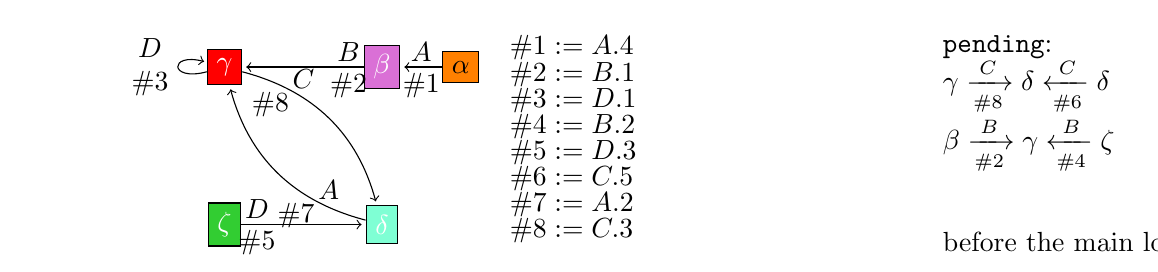
\begin{tikzpicture}[scale=1]       % STEP 0
    \path[use as bounding box] (-2.5, -0.25) rectangle (11.5, 2.5);

    \node[draw,fill=red,text=white] at (0, 2) (R) {$\gamma$};
    \node[draw,fill=LimeGreen,text=white] at (0, 0) (G) {$\zeta$};
    \node[draw,fill=Aquamarine,text=white] at (2, 0) (B) {$\delta$};
    \node[draw,fill=Orchid,text=white] at (2, 2) (K) {$\beta$};
    \node[draw, fill=orange] at (3, 2) (start) {$\alpha$};
    

%   \draw (B) edge[->, loop right] node[right,align=center] {$C$ \\ $\#6$} ();
%   \draw (G) edge[->] node[left,align=center] {$B$ \\ $\#4$} (R);

    \draw (start) edge[->] node[above=-0.5mm] {$A$} node[below=-0.5mm] {\#1} (K);
    \draw (K) edge[->] node[above=-0.5mm, very near start] {$B$} node[below=-0.5mm, very near start] {\#2} (R);
    \draw (B) edge[->, bend left] node[near start, below left=-1mm] {$\#7$} node[near start, above right=-1mm] {$A$} (R);
    \draw (G) edge[->] node[above=-0.5mm, very near start] {$D$} node[below=-0.5mm, very near start] {$\#5$} (B);
    \draw (R) edge[->, loop left] node[left,align=center] {$D$ \\ $\#3$} ();
    \draw (R) edge[->, bend left] node[near start, above right=-1mm] {$C$} node[near start, below left=-1mm] {$\#8$} (B);

\begin{scope}[xshift=-1.5cm,yshift=0.25cm]
    \node[anchor=west] at (5, 2)    {$\#1 := A.4$};
    \node[anchor=west] at (5, 1.66) {$\#2 := B.1$};
    \node[anchor=west] at (5, 1.33) {$\#3 := D.1$};
    \node[anchor=west] at (5, 1)    {$\#4 := B.2$};
    \node[anchor=west] at (5, 0.66) {$\#5 := D.3$};
    \node[anchor=west] at (5, 0.33) {$\#6 := C.5$};
    \node[anchor=west] at (5, 0)    {$\#7 := A.2$};
    \node[anchor=west] at (5,-0.33) {$\#8 := C.3$};

    \node[anchor=west] at (10.5, 2) {\texttt{pending}:};
    \node[anchor=west] at (10.5, 1.5) {$\gamma \xrightarrow[\# 8]{C} \delta \xleftarrow[\# 6]{C} \delta$};
    \node[anchor=west] at (10.5, 0.75) {$\beta \xrightarrow[\#2]{B} \gamma \xleftarrow[\#4]{B} \zeta$};

    \node[anchor=west] at (10.5, -0.5) {before the main loop};
  \end{scope}
\end{tikzpicture}

  \vspace{0.25cm}
  \hrule
  \vspace{0.25cm}
  
  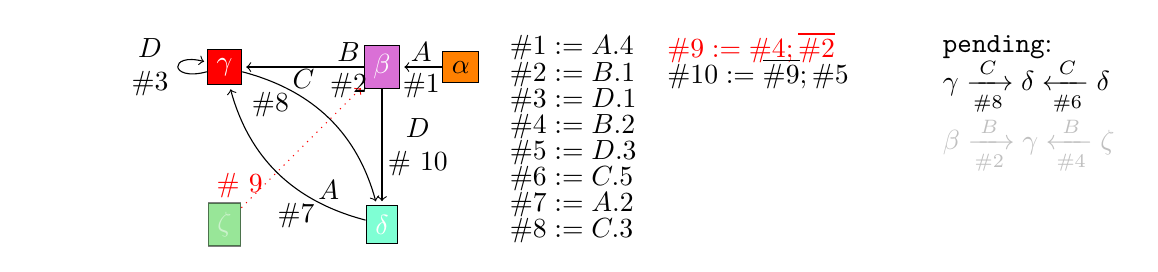
\begin{tikzpicture}[scale=1]      % STEP 1
    \path[use as bounding box] (-2.5, -0.25) rectangle (11.5, 2.5);

    \node[draw,fill=red,text=white] at (0, 2) (R) {$\gamma$};
    \node[draw,semitransparent,fill=LimeGreen,text=white] at (0, 0) (G) {$\zeta$};
    \node[draw,fill=Aquamarine,text=white] at (2, 0) (B) {$\delta$};
    \node[draw,fill=Orchid,text=white] at (2, 2) (K) {$\beta$};
    \node[draw, fill=orange] at (3, 2) (start) {$\alpha$};
    
    \draw (G) edge[red, dotted, ->] node[above left=-2mm, very near start] {\# 9} (K);
    
%   \draw (B) edge[->, loop right] node[right,align=center] {$C$ \\ $\#6$} ();
%   \draw (G) edge[->] node[left,align=center] {$B$ \\ $\#4$} (R);

    \draw (start) edge[->] node[above=-0.5mm] {$A$} node[below=-0.5mm] {\#1} (K);
    \draw (K) edge[->] node[above=-0.5mm, very near start] {$B$} node[below=-0.5mm, very near start] {\#2} (R);
    \draw (B) edge[->, bend left] node[near start, below left=-1mm] {$\#7$} node[near start, above right=-1mm] {$A$} (R);
    \draw (K) edge[->] node[right=-0.5mm, align=center] {$D$ \\ \# 10} (B);
    \draw (R) edge[->, loop left] node[left,align=center] {$D$ \\ $\#3$} ();
    \draw (R) edge[->, bend left] node[near start, above right=-1mm] {$C$} node[near start, below left=-1mm] {$\#8$} (B);

\begin{scope}[xshift=-1.5cm,yshift=0.25cm]
    \node[anchor=west] at (5, 2)    {$\#1 := A.4$};
    \node[anchor=west] at (5, 1.66) {$\#2 := B.1$};
    \node[anchor=west] at (5, 1.33) {$\#3 := D.1$};
    \node[anchor=west] at (5, 1)    {$\#4 := B.2$};
    \node[anchor=west] at (5, 0.66) {$\#5 := D.3$};
    \node[anchor=west] at (5, 0.33) {$\#6 := C.5$};
    \node[anchor=west] at (5, 0)    {$\#7 := A.2$};
    \node[anchor=west] at (5,-0.33) {$\#8 := C.3$};

    \begin{scope}[xshift=2cm,yshift=2.66cm]
    \node[anchor=west,red] at (5,-0.66) {$\#9 := \# 4; \overline{\# 2}$};
    \node[anchor=west] at (5,-1) {$\#10 := \overline{\# 9}; \# 5$};
  \end{scope}
  
    \node[anchor=west] at (10.5, 2) {\texttt{pending}:};
    \node[anchor=west] at (10.5, 1.5) {$\gamma \xrightarrow[\# 8]{C} \delta \xleftarrow[\# 6]{C} \delta$};
    \node[anchor=west,lightgray] at (10.5, 0.75) {$\beta \xrightarrow[\#2]{B} \gamma \xleftarrow[\#4]{B} \zeta$};
\end{scope}
  \end{tikzpicture}

  \vspace{0.25cm}
  \hrule
  \vspace{0.25cm}

  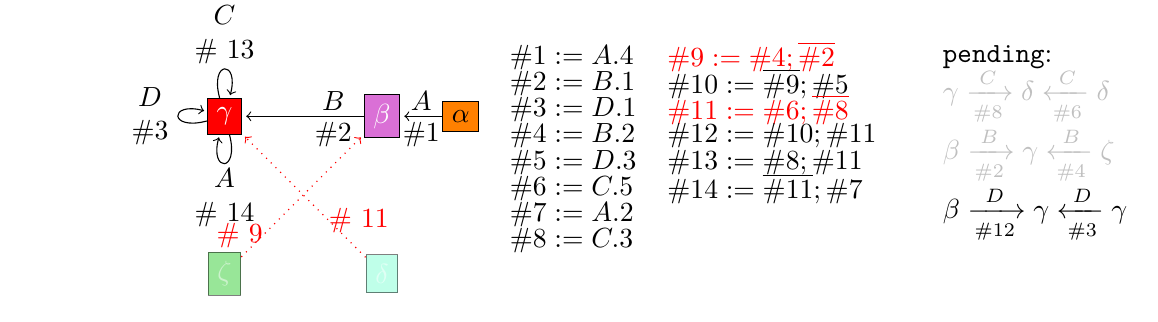
\begin{tikzpicture}[scale=1]      % STEP 2 (new)
    \path[use as bounding box] (-2.5, -0.25) rectangle (11.5, 3.125);

    \node[draw,fill=red,text=white] at (0, 2) (R) {$\gamma$};
    \node[draw,semitransparent,fill=LimeGreen,text=white] at (0, 0) (G) {$\zeta$};
    \node[draw,semitransparent,fill=Aquamarine,text=white] at (2, 0) (B) {$\delta$};
    \node[draw,fill=Orchid,text=white] at (2, 2) (K) {$\beta$};
    \node[draw, fill=orange] at (3, 2) (start) {$\alpha$};
    
    \draw (G) edge[red, dotted, ->] node[above left=-2mm, very near start] {\# 9} (K);
    \draw (B) edge[red, dotted, ->] node[above right=-2mm, near start] {\# 11} (R);
    
%   \draw (B) edge[->, loop right] node[right,align=center] {$C$ \\ $\#6$} ();
%   \draw (G) edge[->] node[left,align=center] {$B$ \\ $\#4$} (R);
%   \draw (R) edge[->, bend left] node[near start, above right=-1mm] {$C$} node[near start, below left=-1mm] {$\#8$} (B);
%   \draw (B) edge[->, bend left] node[near start, below left=-1mm] {$\#7$} node[near start, above right=-1mm] {$A$} (R);
%   \draw (K) edge[->] node[right=-0.5mm, align=center] {$D$ \\ \# 10} (B);
   \draw (R) edge[->, loop left] node[left,align=center] {$D$ \\ $\#3$} ();
    
    \draw (start) edge[->] node[above=-0.5mm] {$A$} node[below=-0.5mm] {\#1} (K);
    \draw (K) edge[->] node[above=-0.5mm, near start] {$B$} node[below=-0.5mm, near start] {\#2} (R);
    \draw (R) edge[->, loop above] node[above=-0.5mm,align=center] {$C$ \\ \# 13} ();
    \draw (R) edge[->, loop below] node[below=-0.5mm,align=center] {$A$ \\ \# 14} ();
%    \draw[->] (K.north west) .. controls (1.5, 3) and (0.5, 3) .. node[above=-0.5mm] {$D$} node[below] {\# 12} (R.north east);      


    \begin{scope}[xshift=-1.5cm,yshift=0.75cm]
    \node[anchor=west] at (5, 2)    {$\#1 := A.4$};
    \node[anchor=west] at (5, 1.66) {$\#2 := B.1$};
    \node[anchor=west] at (5, 1.33) {$\#3 := D.1$};
    \node[anchor=west] at (5, 1)    {$\#4 := B.2$};
    \node[anchor=west] at (5, 0.66) {$\#5 := D.3$};
    \node[anchor=west] at (5, 0.33) {$\#6 := C.5$};
    \node[anchor=west] at (5, 0)    {$\#7 := A.2$};
    \node[anchor=west] at (5,-0.33) {$\#8 := C.3$};

    \begin{scope}[xshift=2cm,yshift=2.66cm]    
    \node[anchor=west,red] at (5,-0.66) {$\#9 := \# 4; \overline{\# 2}$};
    \node[anchor=west] at (5,-1) {$\#10 := \overline{\# 9}; \# 5$};
    \node[anchor=west,red] at (5,-1.33) {$\#11 := \# 6; \overline{\# 8}$};
    \node[anchor=west] at (5,-1.66) {$\#12 := \# 10 ; \# 11$};
    \node[anchor=west] at (5,-2) {$\#13 := \# 8 ; \# 11$};
    \node[anchor=west] at (5,-2.33) {$\#14 := \overline{\# 11} ; \# 7$};
    \end{scope}

    \node[anchor=west] at (10.5, 2) {\texttt{pending}:};
    \node[anchor=west,lightgray] at (10.5, 1.5) {$\gamma \xrightarrow[\# 8]{C} \delta \xleftarrow[\# 6]{C} \delta$};
    \node[anchor=west,lightgray] at (10.5, 0.75) {$\beta \xrightarrow[\#2]{B} \gamma \xleftarrow[\#4]{B} \zeta$};
    \node[anchor=west] at (10.5, 0) {$\beta \xrightarrow[\#12]{D} \gamma \xleftarrow[\#3]{D} \gamma$};
  \end{scope}
\end{tikzpicture}

  \vspace{0.25cm}
  \hrule
  \vspace{0.25cm}
  
  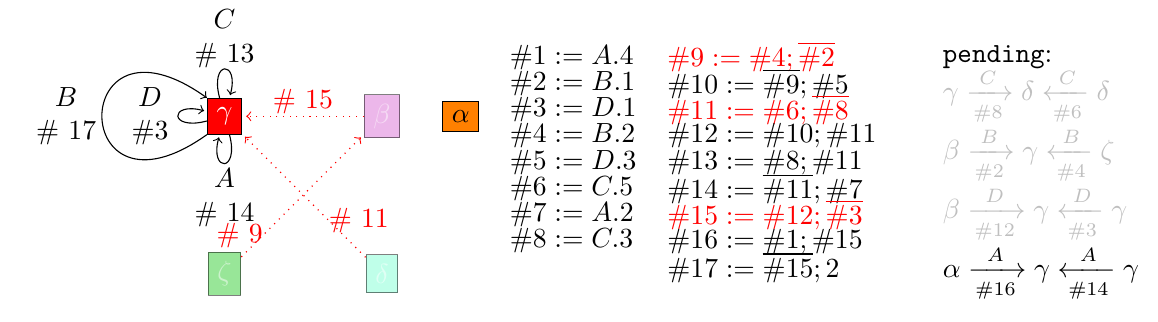
\begin{tikzpicture}[scale=1]      % STEP 3
    \path[use as bounding box] (-2.5, -0.25) rectangle (11.5, 3.125);
    
   \node[draw,fill=red,text=white] at (0, 2) (R) {$\gamma$};
    \node[draw,semitransparent,fill=LimeGreen,text=white] at (0, 0) (G) {$\zeta$};
    \node[draw,semitransparent,fill=Aquamarine,text=white] at (2, 0) (B) {$\delta$};
    \node[draw,semitransparent,fill=Orchid,text=white] at (2, 2) (K) {$\beta$};
    \node[draw, fill=orange] at (3, 2) (start) {$\alpha$};
    
    \draw (G) edge[red, dotted, ->] node[above left=-2mm, very near start] {\# 9} (K);
    \draw (B) edge[red, dotted, ->] node[above right=-2mm, near start] {\# 11} (R);
    \draw (K) edge[red, dotted, ->] node[above=-1mm] {\# 15} (R);
    
%   \draw (B) edge[->, loop right] node[right,align=center] {$C$ \\ $\#6$} ();
%   \draw (G) edge[->] node[left,align=center] {$B$ \\ $\#4$} (R);
%   \draw (R) edge[->, bend left] node[near start, above right=-1mm] {$C$} node[near start, below left=-1mm] {$\#8$} (B);
%   \draw (B) edge[->, bend left] node[near start, below left=-1mm] {$\#7$} node[near start, above right=-1mm] {$A$} (R);
%   \draw (K) edge[->] node[right=-0.5mm, align=center] {$D$ \\ \# 10} (B);
%   \draw (K) edge[->] node[above=-0.5mm, near start] {$B$} node[below=-0.5mm, near start] {\#2} (R);
    
    \draw (R) edge[->, loop left] node[left,align=center] {$D$ \\ $\#3$} ();
    \draw (R) edge[->, loop above] node[above=-1mm,align=center] {$C$ \\ \# 13} ();
    \draw (R) edge[->, loop below] node[below=-0.5mm,align=center] {$A$ \\ \# 14} ();
%    \draw[->] (start.north west) .. controls (3.5, 3) and (0.5, 3) .. node[above=-0.5mm] {$A$} node[below] {\# 16} (R.north east);      
    \draw[->] (R.south west) .. controls (-2, 0.5) and (-2, 3.5) .. node[left=-0.5mm, align=center] {$B$ \\ \# 17} (R.north west);

    
    \begin{scope}[xshift=-1.5cm,yshift=0.75cm]
    \node[anchor=west] at (5, 2)    {$\#1 := A.4$};
    \node[anchor=west] at (5, 1.66) {$\#2 := B.1$};
    \node[anchor=west] at (5, 1.33) {$\#3 := D.1$};
    \node[anchor=west] at (5, 1)    {$\#4 := B.2$};
    \node[anchor=west] at (5, 0.66) {$\#5 := D.3$};
    \node[anchor=west] at (5, 0.33) {$\#6 := C.5$};
    \node[anchor=west] at (5, 0)    {$\#7 := A.2$};
    \node[anchor=west] at (5,-0.33) {$\#8 := C.3$};
    
    \begin{scope}[xshift=2cm,yshift=2.66cm]
      \node[anchor=west,red] at (5,-0.66) {$\#9 := \# 4; \overline{\# 2}$};
      \node[anchor=west] at (5,-1) {$\#10 := \overline{\# 9}; \# 5$};
    \node[anchor=west,red] at (5,-1.33) {$\#11 := \# 6; \overline{\# 8}$};
    \node[anchor=west] at (5,-1.66) {$\#12 := \# 10 ; \# 11$};
    \node[anchor=west] at (5,-2) {$\#13 := \# 8 ; \# 11$};
    \node[anchor=west] at (5,-2.33) {$\#14 := \overline{\# 11} ; \# 7$};
    \node[anchor=west,red] at (5,-2.66) {$\#15 := \#12; \overline{\# 3}$};
    \node[anchor=west] at (5,-3) {$\#16 := \#1; \# 15$};
    \node[anchor=west] at (5,-3.33) {$\#17 := \overline{\# 15}; 2$};
    \end{scope}

    \node[anchor=west] at (10.5, 2) {\texttt{pending}:};
    \node[anchor=west,lightgray] at (10.5, 1.5) {$\gamma \xrightarrow[\# 8]{C} \delta \xleftarrow[\# 6]{C} \delta$};
    \node[anchor=west,lightgray] at (10.5, 0.75) {$\beta \xrightarrow[\#2]{B} \gamma \xleftarrow[\#4]{B} \zeta$};
    \node[anchor=west,lightgray] at (10.5, 0) {$\beta \xrightarrow[\#12]{D} \gamma \xleftarrow[\#3]{D} \gamma$};
    \node[anchor=west] at (10.5, -0.75) {$\alpha \xrightarrow[\# 16]{A} \gamma \xleftarrow[\# 14]{A} \gamma$};
  \end{scope}
\end{tikzpicture}

  \vspace{0.25cm}
  \hrule
  %\vspace{0.25cm}
  
  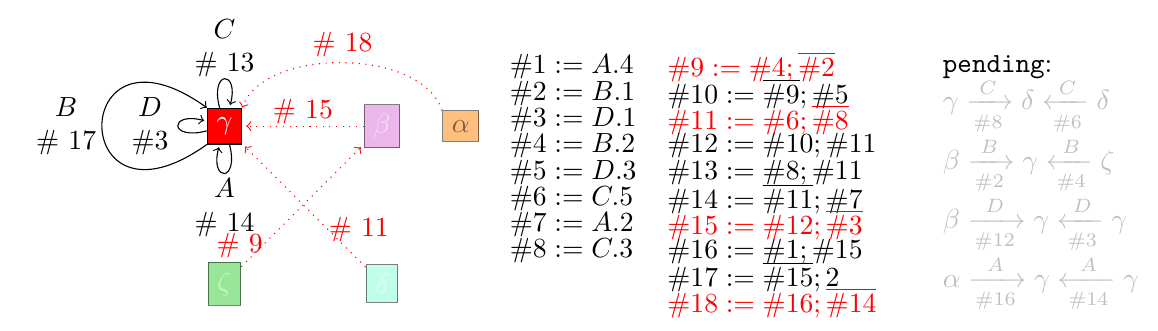
\begin{tikzpicture}[scale=1]      % STEP 4 (final)
    \path[use as bounding box] (-2.5, -0.25) rectangle (11.5, 3.25);

    \node[draw,fill=red,text=white] at (0, 2) (R) {$\gamma$};
    \node[draw,semitransparent,fill=LimeGreen,text=white] at (0, 0) (G) {$\zeta$};
    \node[draw,semitransparent,fill=Aquamarine,text=white] at (2, 0) (B) {$\delta$};
    \node[draw,semitransparent,fill=Orchid,text=white] at (2, 2) (K) {$\beta$};
    \node[draw,semitransparent,fill=orange] at (3, 2) (start) {$\alpha$};
    
    \draw (G) edge[red, dotted, ->] node[above left=-2mm, very near start] {\# 9} (K);
    \draw (B) edge[red, dotted, ->] node[above right=-2mm, near start] {\# 11} (R);
    \draw (K) edge[red, dotted, ->] node[above=-1mm] {\# 15} (R);
    \draw[red,dotted,->] (start.north west) .. controls (2.5, 3) and (0.5, 3) .. node[above=-0.5mm] {\# 18} (R.north east);      

    
%   \draw (B) edge[->, loop right] node[right,align=center] {$C$ \\ $\#6$} ();
%   \draw (G) edge[->] node[left,align=center] {$B$ \\ $\#4$} (R);
%   \draw (R) edge[->, bend left] node[near start, above right=-1mm] {$C$} node[near start, below left=-1mm] {$\#8$} (B);
%   \draw (B) edge[->, bend left] node[near start, below left=-1mm] {$\#7$} node[near start, above right=-1mm] {$A$} (R);
%   \draw (K) edge[->] node[right=-0.5mm, align=center] {$D$ \\ \# 10} (B);
%   \draw (K) edge[->] node[above=-0.5mm, near start] {$B$} node[below=-0.5mm, near start] {\#2} (R);
    
    \draw (R) edge[->, loop left] node[left,align=center] {$D$ \\ $\#3$} ();
    \draw (R) edge[->, loop above] node[above=-1mm,align=center] {$C$ \\ \# 13} ();
    \draw (R) edge[->, loop below] node[below=-0.5mm,align=center] {$A$ \\ \# 14} ();
    \draw[->] (R.south west) .. controls (-2, 0.5) and (-2, 3.5) .. node[left=-0.5mm, align=center] {$B$ \\ \# 17} (R.north west);
    
    \begin{scope}[xshift=-1.5cm,yshift=0.75cm]
    \node[anchor=west] at (5, 2)    {$\#1 := A.4$};
    \node[anchor=west] at (5, 1.66) {$\#2 := B.1$};
    \node[anchor=west] at (5, 1.33) {$\#3 := D.1$};
    \node[anchor=west] at (5, 1)    {$\#4 := B.2$};
    \node[anchor=west] at (5, 0.66) {$\#5 := D.3$};
    \node[anchor=west] at (5, 0.33) {$\#6 := C.5$};
    \node[anchor=west] at (5, 0)    {$\#7 := A.2$};
    \node[anchor=west] at (5,-0.33) {$\#8 := C.3$};

    \begin{scope}[xshift=2cm,yshift=2.66cm]
    \node[anchor=west,red] at (5,-0.66) {$\#9 := \# 4; \overline{\# 2}$};
    \node[anchor=west] at (5,-1) {$\#10 := \overline{\# 9}; \# 5$};
    \node[anchor=west,red] at (5,-1.33) {$\#11 := \# 6; \overline{\# 8}$};
    \node[anchor=west] at (5,-1.66) {$\#12 := \# 10 ; \# 11$};
    \node[anchor=west] at (5,-2) {$\#13 := \# 8 ; \# 11$};
    \node[anchor=west] at (5,-2.33) {$\#14 := \overline{\# 11} ; \# 7$};
    \node[anchor=west,red] at (5,-2.66) {$\#15 := \#12; \overline{\# 3}$};
    \node[anchor=west] at (5,-3) {$\#16 := \#1; \# 15$};
    \node[anchor=west] at (5,-3.33) {$\#17 := \overline{\# 15}; 2$};
    \node[anchor=west,red] at (5,-3.66) {$\#18 := \#16; \overline{\# 14}$};
    \end{scope}
  
    \node[anchor=west] at (10.5, 2) {\texttt{pending}:};
    \node[anchor=west,lightgray] at (10.5, 1.5) {$\gamma \xrightarrow[\# 8]{C} \delta \xleftarrow[\# 6]{C} \delta$};
    \node[anchor=west,lightgray] at (10.5, 0.75) {$\beta \xrightarrow[\#2]{B} \gamma \xleftarrow[\#4]{B} \zeta$};
    \node[anchor=west,lightgray] at (10.5, 0) {$\beta \xrightarrow[\#12]{D} \gamma \xleftarrow[\#3]{D} \gamma$};
    \node[anchor=west,lightgray] at (10.5, -0.75) {$\alpha \xrightarrow[\# 16]{A} \gamma \xleftarrow[\# 14]{A} \gamma$};
  \end{scope}
\end{tikzpicture}
\end{center}

\caption{Step-by-step illustration of the construction of an exit path. The plain
  edges are ``hot''. The dotted edges represent are the extra spanning edges). \label{fig:path-finding}}
\end{figure}


\section{Conclusion: a daunting open problem}

Checking if a context-free language is empty is non only decidable, but can be
done in polynomial time. For this reason, it was clear from the outset that
recursive mazes could not pose a major computational problem.

However, checking emptiness of the intersection of \emph{two} context-free
languages is undecidable (this enables the simulation of an arbitrary Turing
machine). Therefore, it could very well be that trying to get out of \emph{two}
recursive mazes simultaneously might be difficult. This problem can be thought
of as follows: suppose you have an application to play recursive mazes
(\verb|\begin{shameless-advertisement}|such as the one we designed, available at
  \url{https://github.com/orelcosseron/Fractal-Maze-Python}\verb|\end{shameless-advertisement}|). In
such a game, the mazes are orthogonal: paths are either horizontal or
vertical. The player controls the location of a sprite using arrow keys, as is
common in ``top down'' adventure games, such as \emph{The Legend of
  Zelda}. Moving towards a wall does nothing: the sprite cannot cross the
wall.

\begin{figure}
\begin{center}
  \includegraphics[width=0.49\textwidth]{screenshot_Alice.png}
  \includegraphics[width=0.49\textwidth]{screenshot_square.png}
\end{center}
\caption{\label{fig:two} Solving two mazes at the same time---with a single
  keyboard. Is it decidable? The player is represented by a blue dot, and its
  current path is shown by a blue or red line.}
\end{figure}

Now suppose that \emph{two} instances of the application are launched, with two
different mazes, and that \emph{both} applications receive the same keyboard
inputs (see Fig.~\ref{fig:two}). In the situation shown in the figure, going
down does nothing; going up moves the sprite in the right maze; going left moves
the sprite in the left maze; going right moves the sprite in both mazes. Given
the geometric description of two mazes, the question is to decide if there is a
(finite) sequence of keyboard inputs that exits both mazes.

It is not completely obvious that this problem is even decidable (we may get
away with it because of the severe restrictions on the class of context-free
languages associated to recursive mazes). In any case, this is an exciting
perspective for future work

\bibliography{biblio}

\end{document}

%%% Local Variables:
%%% ispell-local-dictionary: "english"
%%% eval: (flyspell-mode 1)
%%% eval: (reftex-mode 1)
%%% End: